
\documentclass[10pt, a4paper]{report}
\usepackage[utf8]{inputenc}
\usepackage[margin=2cm]{geometry}
\usepackage{graphicx}
\usepackage{titlesec, color}
\definecolor{gray75}{gray}{0.75}
\newcommand{\hsp}{\hspace{20pt}}
\usepackage[svgnames]{xcolor}
\usepackage{float}
\usepackage{multirow}
\usepackage{multicol}
\setlength{\columnsep}{1cm}
\usepackage[italian]{babel}
\usepackage{bookmark}
\hypersetup{pdfborder = 0 0 0}
\titlespacing{\chapter}{0pt}{0pt}{40pt}
\usepackage{lipsum}
\usepackage{amsmath}
\usepackage{csquotes}
\usepackage[utf8]{inputenc}
\usepackage[T1]{fontenc}
\usepackage{tikz}
\usepackage{enumitem}
\usepackage{etoolbox}
\usepackage{imfellEnglish}

% Define custom colors for the D&D theme
\definecolor{DNDGold}{rgb}{0.698, 0.549, 0.278} % Darker Gold #B28C47
\definecolor{DNDDarkBlue}{HTML}{4C788A} % Darker Blue #2C4A5D
\definecolor{DNDGray}{rgb}{0.2, 0.2, 0.2} % Dark gray for text
\definecolor{DNDWhite}{rgb}{253, 253, 253}

% Custom part title format
\titleformat{\part}[display]
{\Huge\color{DNDDarkBlue}\centering} % Centered, bold, dark blue font
{\textcolor{DNDDarkBlue}{Parte \textcolor{DNDGold}{\thepart}}} % "Parte" + part number in gold
{0em} % No space between number and title
{\vspace{0.5cm}\Huge\scshape} % Title in small caps
[] % Rule below title

% Custom chapter title format
\titleformat{\chapter}[block]
{\huge\color{DNDDarkBlue}} % Slightly smaller than \part
{\textcolor{DNDGold}{\thechapter}} % Chapter number in gold
{1em} % Space between number and title
{\huge\scshape} % Title in small caps
[\vspace{-0.16em}\titlerule] % Rule below title

% Custom section title format
\titleformat{\section}[block]
{\Large\color{DNDDarkBlue}} % Smaller font than \chapter
{\textcolor{DNDGold}{\thesection}} % Section number in gold
{1em} % Space between number and title
{\Large\scshape} % Title in small caps
[\vspace{-0.16em}\titlerule] % Thin rule below title


% Custom subsubsection title format
\titleformat{\subsection}[block]
{\fontsize{13}{16}\color{DNDDarkBlue}} % Normal font, dark blue color, bold
{\textcolor{DNDGold}{\thesubsection}} % Subsection number
{1em} % Space between number and title
{\fontsize{13}{17}\scshape}
[] % No rule below

% Custom subsubsection title format
\titleformat{\subsubsection}[block]
{\large\bfseries\color{DNDDarkBlue}\bfseries} % Normal font, dark blue color, bold
{\textcolor{DNDGold}{\thesubsubsection}} % Subsubsection number
{1em} % Space between number and title
{\large\bfseries}
[] % No rule below

% Global configuration for itemize
\setlist[itemize]{label=\small$\diamond$}  % Set smaller bullets for all itemize lists

\graphicspath{{imgs/}}

\DeclareUnicodeCharacter{011F}{\u{g}} % g breve
\DeclareUnicodeCharacter{0259}{\u{e}} % schwa
\DeclareUnicodeCharacter{015F}{\c{s}} % s con cediglia


\begin{document}
	
\begin{titlepage}
	\begin{tikzpicture}[remember picture, overlay]
		\node at (current page.center) {
			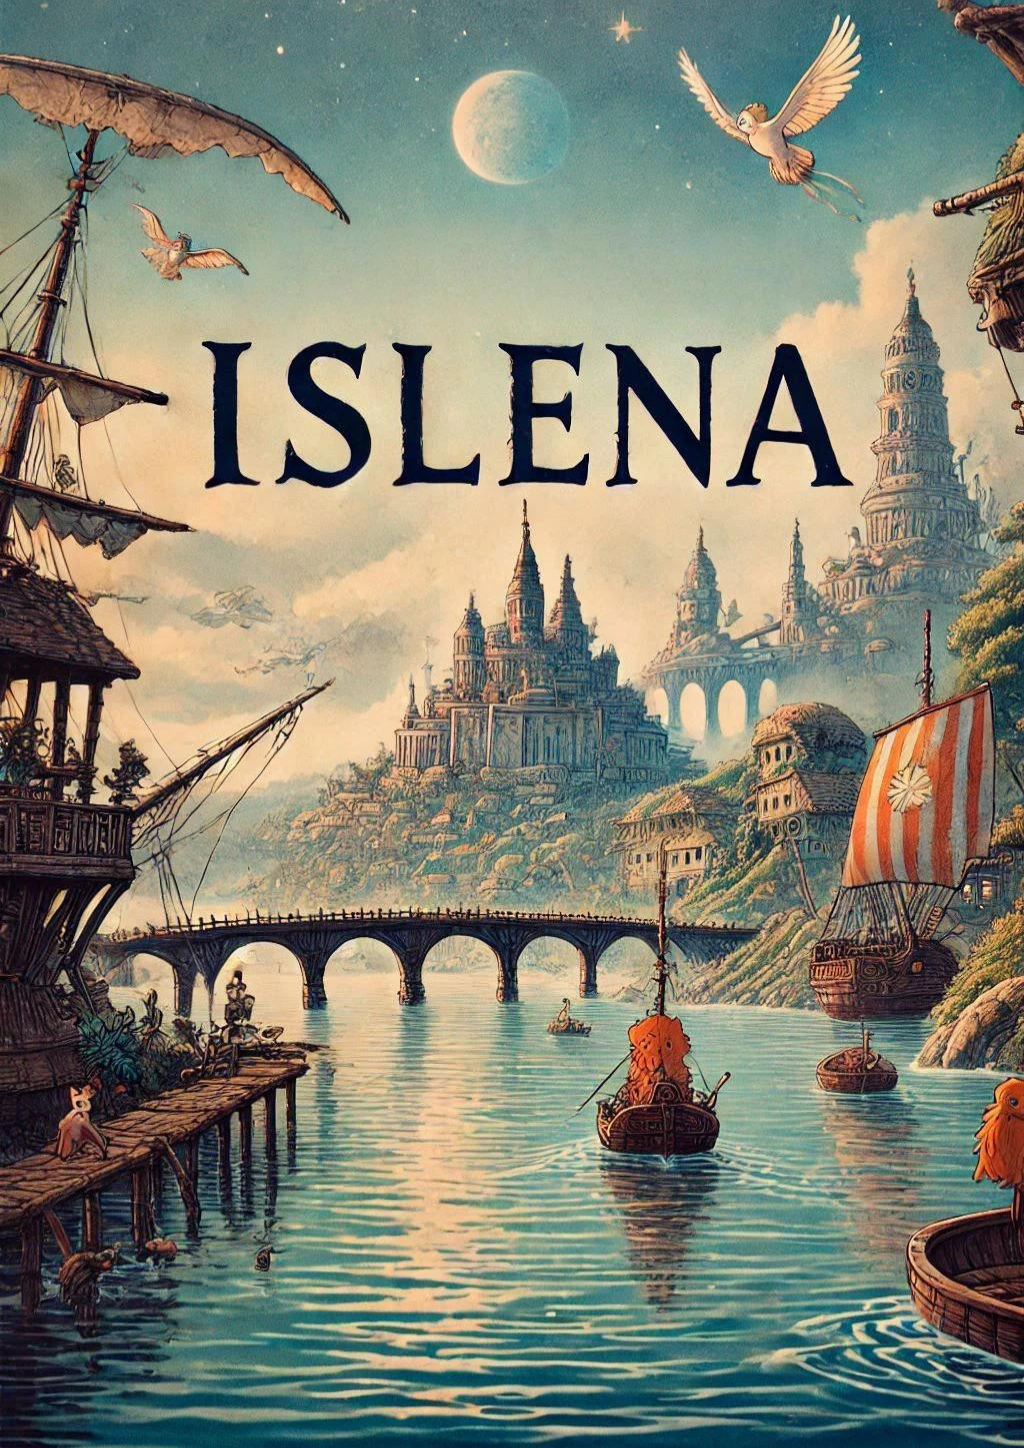
\includegraphics[width=\paperwidth, height=\paperheight]{titlepageislena1.jpg}
		};
	\end{tikzpicture}

\centering

\begin{tikzpicture}[remember picture, overlay]
	\node at ([yshift=-3.5cm]current page.north) {
		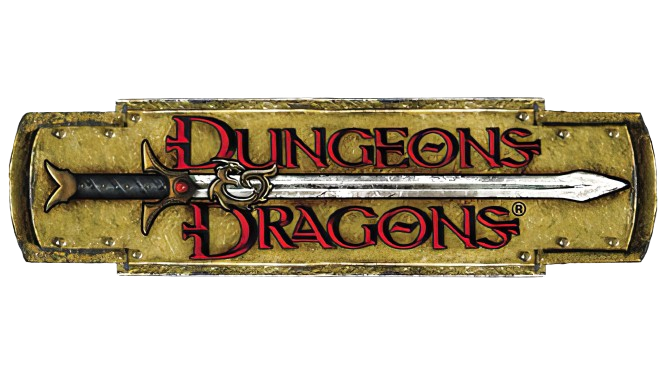
\includegraphics[scale=0.40]{dnd1.png}
	};
\end{tikzpicture}
\vspace{11.5cm}
\par
{\Huge\scshape\textcolor{MintCream}{Guida \\
			all'Ambientazione}}
\vfill
\par
{\textbf{\textcolor{MintCream}{Manu-ale assolutamente non ufficiale}}}
\vfill
\textcolor{MintCream}{\textbf{\today}}
\end{titlepage}

\pagecolor{DNDWhite}

%\begin{multicols}{2}
\tableofcontents
%\end{multicols}

\newpage
\clearpage
\section{Introduzione}
Questo documento vuole essere una guida all'ambientazione che useremo nella campagna. Ho cercato di creare una cosmologia circa originale che rimane abbastanza legata alla cosmologia canonica di D\&D per evitare problemi con incantesimi, spostamenti tra piani e cose simili, divinità più o meno serie e una storia del continente per niente freebootata.\\
La campagna sarà ambientata nello mirabilantes continente di Islena, non è dato sapere su quale pianeta e per quanto vi riguarda non è dato sapere manco se esistono i pianeti. \\
La prima parte del documento è focalizzata sulla cosmologia mentre nella seconda verrà descritto il continente nello specifico. C'è una terza parte in cui si affrontano i cambiamenti e le aggiunte alla regole di gioco vere e proprie.\\
\\
Ringrazio in primis Bicchan, aka mia sorella, per i contributi alle idee per la cosmologia e la campagna stessa; E ringrazio voi, che avete contribuito con i vostri background alla creazione dell'ambientazione e che sarete così gentili da giocare qualsiasi merdata riuscirò a DMare. Un ringraziamento in particolare va al calva (mi è stato segnalato di scriverlo con la minuscola) per le gentili segnalazioni di svariati errori.\\
\\
PS: Se trovate cazzate di ortografia, robe che non tornano o che non capite e altri errori siete pregati di segnalarli grazie.  \\
\\
\\
- Emipano


\part{Cosmologia}
\chapter{Struttura della Cosmologia}
\begin{multicols}{2}
\section{Introduzione}
 Per semplificare le cose e evitare problemi non ci allontaneremo dalla struttura \enquote{a piani} della cosmologia canonica descritta nel Manuale del Dungeon Master, ovviamente ho creato nuovi piani a sostituire quelli canonici ma manterremo quelli principali e legati al funzionamento di incantesimi vari. Nonostante ciò alcuni incantesimi potrebbero avere funzionamenti diversi dal normale, a causa di alcuni comportamenti dei piani che non sono necessariamente riportati in questo documento.
\section{Origine del Cosmo}
Prima di elencare e descrivere ogni piano racconto la storia dell'origine del cosmo per avere un'idea generale della struttura della cosmologia e anche perché mi andava e ormai l'avevo inventata quindi ve la puppate. Sia ben chiaro che questa è la versione che gli Dei raccontano dell'origine del mondo, nulla vieta che pg e png credano a versioni diverse. 
\\
\begin{verse}
\textit{Prima del Tempo vi era il Mare di Stelle e nel Mare di Stelle vi nuotava il Nuotatore, essere munito di corpo e mente non consapevole.
Quando il Nuotatore acquistò consapevolezza pensò e dal suo pensiero si generarono una differenza spaziale e una differenza temporale. La differenza spaziale era un'isola su cui riposare il corpo stanco, diversa dal Mare di Stelle; la differenza temporale distingueva il prima dal dopo. Nacquero così Spazio e Tempo. Data l'esistenza del Tempo il Nuotatore non poteva non annoiarsi da solo sulla sua isola tutta uguale e pensò ancora una volta. Dal suo pensiero nacque la differenza prima del mondo: il Nuotatore stesso si divise in Bene e Male. Il forte contrasto tra le due entità portò ad un inevitabile scontro. Le enormi forze in gioco durante la battaglia causarono alla spaccatura dell'isola in tre porzioni: il Fukai dove rimase il Male, il Takai dove rimase il Bene e in tra le due il Tatakai dove rimase il caos della battaglia. Nel Fukai nacquero le creature immonde mentre le creature celestiali sono figlie del Takai.
Nel Tatakai col tempo si calmò il caos e da esso si formarono i Titani Elementali. L'unione dei Titani generò il Mondo dove vivono le creature mortali. I figli Dei Titani furono gli Dei e i figli degli Dei furono altri Dei.}
\end{verse}
\vspace{0.5cm}
\section{I Piani}
In questa sezione saranno descritti brevemente i piani. Quelli principali sono per la maggior parte identici a quelli canonici perché chi me lo fa fa di cambiarli e soprattutto non ho intenzione di creare casini.
\subsection*{Mare di Stelle}
Il Mare di Stelle è lo spazio tra i piani, prende dunque il posto del Piano Astrale.\\
\\
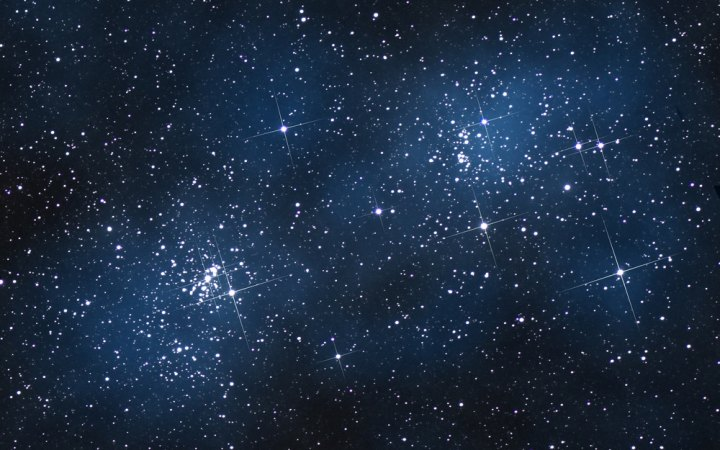
\includegraphics[width=6cm]{stars.jpeg}\\
\\
Il Mare di Stelle si presenta come un'infinita distesa di \enquote*{acqua} calmissima, sovrastata da un magnifico cielo stellato che si riflette perfettamente sulla superficie d'acqua. L'acqua non sembra avere profondità e non è bagnata. I tratti sono:
\begin{itemize}
	\item Assenza di gravità
	\item Assenza di tempo
	\item Dimensioni infinite
	\item Statico
	\item Nessun elemento dominante
	\item Allineamento neutrale
	\item Magia normale
Per il resto fare riferimento al Piano Astrale.
\end{itemize}
\subsection*{Piano Materiale, Etereo e delle Ombre}
Questi piani sono identici a quelli canonici; fare riferimento alla Guida del Dungeon Master.
\subsection*{I Titani Elementali}
In questa cosmologia i Piani Interni diventano delle creature titaniche che funzionano come veri e propri piani adiacenti al Tatakai (o meglio ci vivono sopra, dal punto di vista dei piani si considerano adiacenti). I Titani sono i seguenti:
\begin{itemize}
\item Titano dell'Aria
\item Titano dell'Acqua
\item Titano della Terra
\item Titano del Fuoco
\item Titano dell'Energia Positiva
\item Titano dell'Energia Negativa
\end{itemize}
Anche in questo caso fare riferimento ai Piani Interni canonici ad eccezione del fatto che i Titani sono piani auto-contenuti.
\subsection*{Il Tatakai}
Il Tatakai è il piano in cui vivono le divinità. Alcune divinità sono state cacciate o hanno creato o hanno reso proprio un piano ma occasionalmente anch'esse si trovano qui. Nel Tatakai vivono anche divinità minori e semi-divinità.\\
Il paesaggio è caratterizzato da maestose montagne rocciose sulle quali sorgono degli edifici di architettura ispirata all'architettura greca.\\
Dal Tatakai è possibile vedere i Titani poiché essi lo abitano, tuttavia queste creature sono talmente immense che solo una loro porzione è visibile mentre la maggior parte del loro corpo supera ed è coperta dalle nuvole.\\
\\
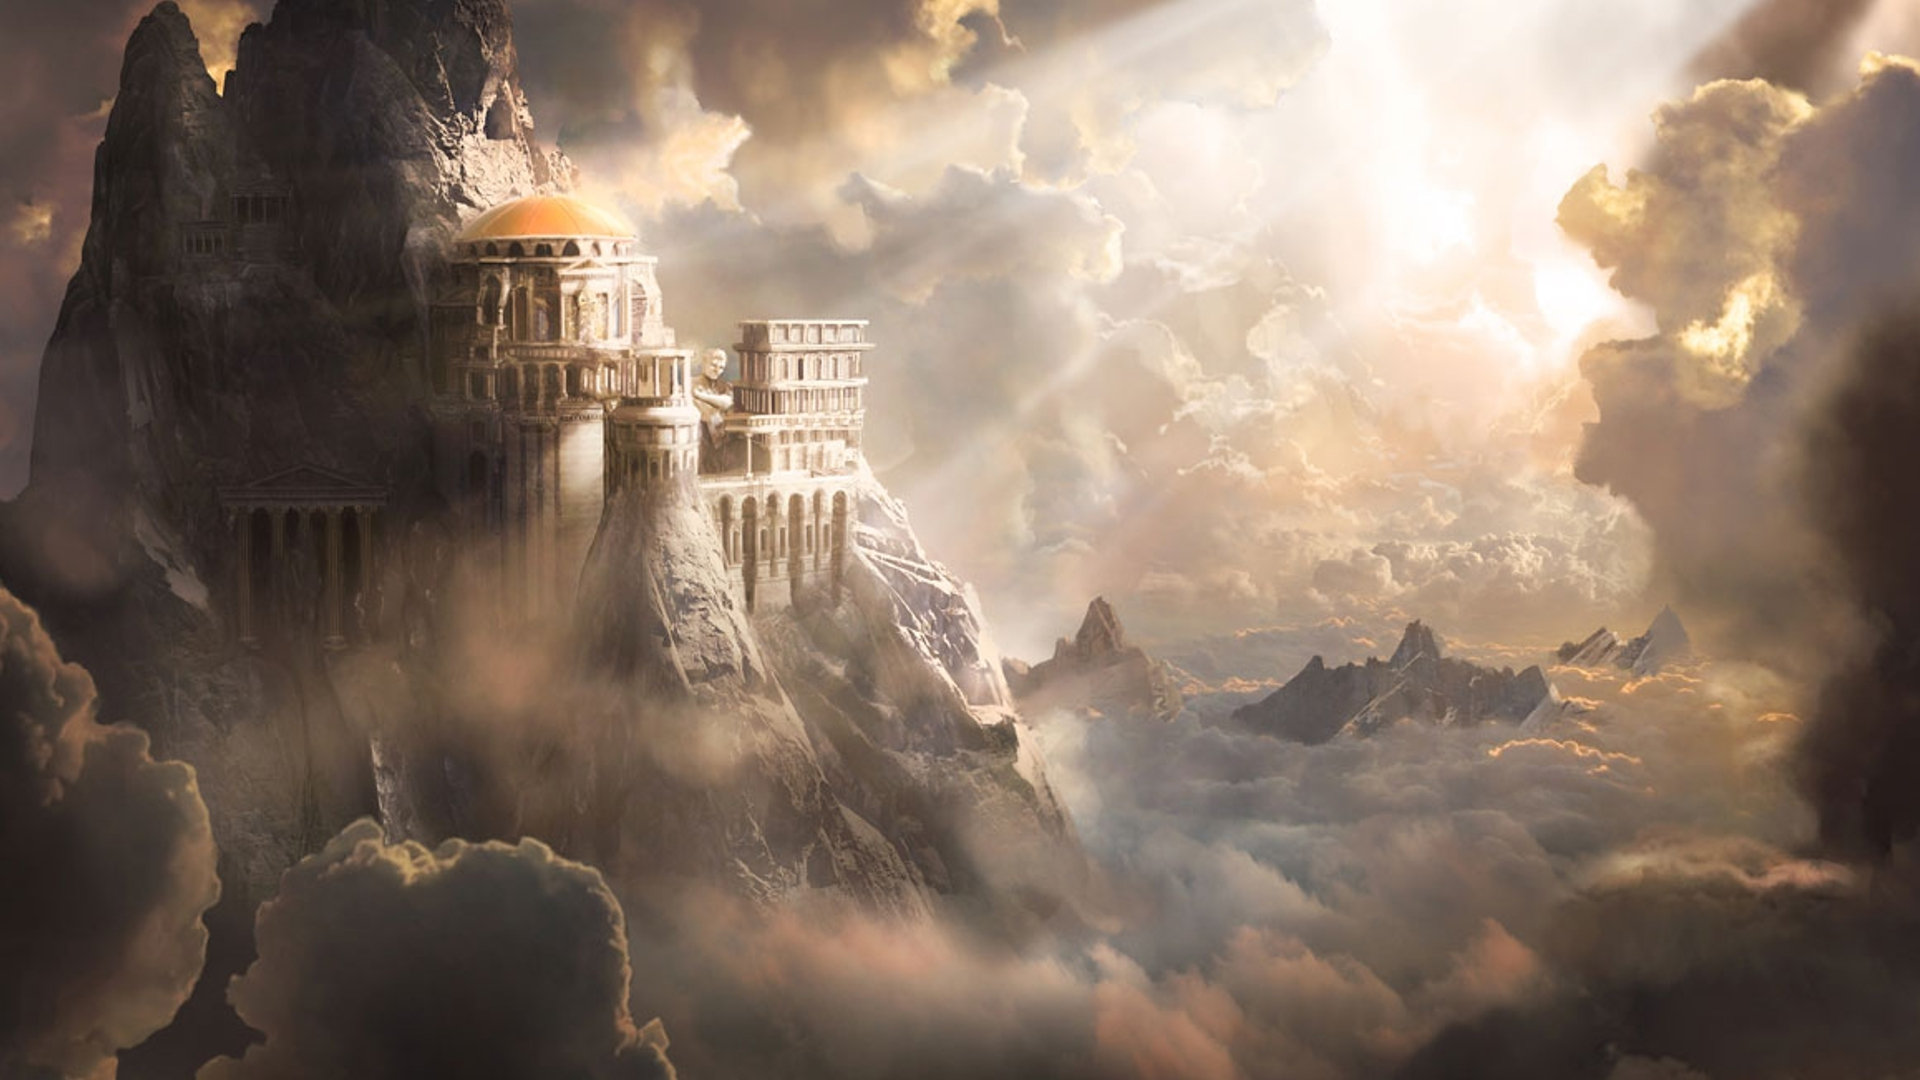
\includegraphics[width = 6cm]{tatakai.png}\\
\\
Il Tatakai è caratterizzato dai seguenti tratti:
\begin{itemize}
	\item Gravità normale
	\item Tempo normale
	\item Dimensioni Infinite
	\item Plasmabile divino
	\item Nessun elemento dominante
	\item Allineamento neutrale
	\item Magia normale
\end{itemize}

\subsection*{Takai}
Il Takai è il piano dove regna il bene. Qui risiedono le creature celestiali e gli esterni di allineamento buono. L'ambiente è caratterizzato da altipiani erbosi percorsi da fiumi e ruscelli che si risolvono in svariate cascate.\\
\\
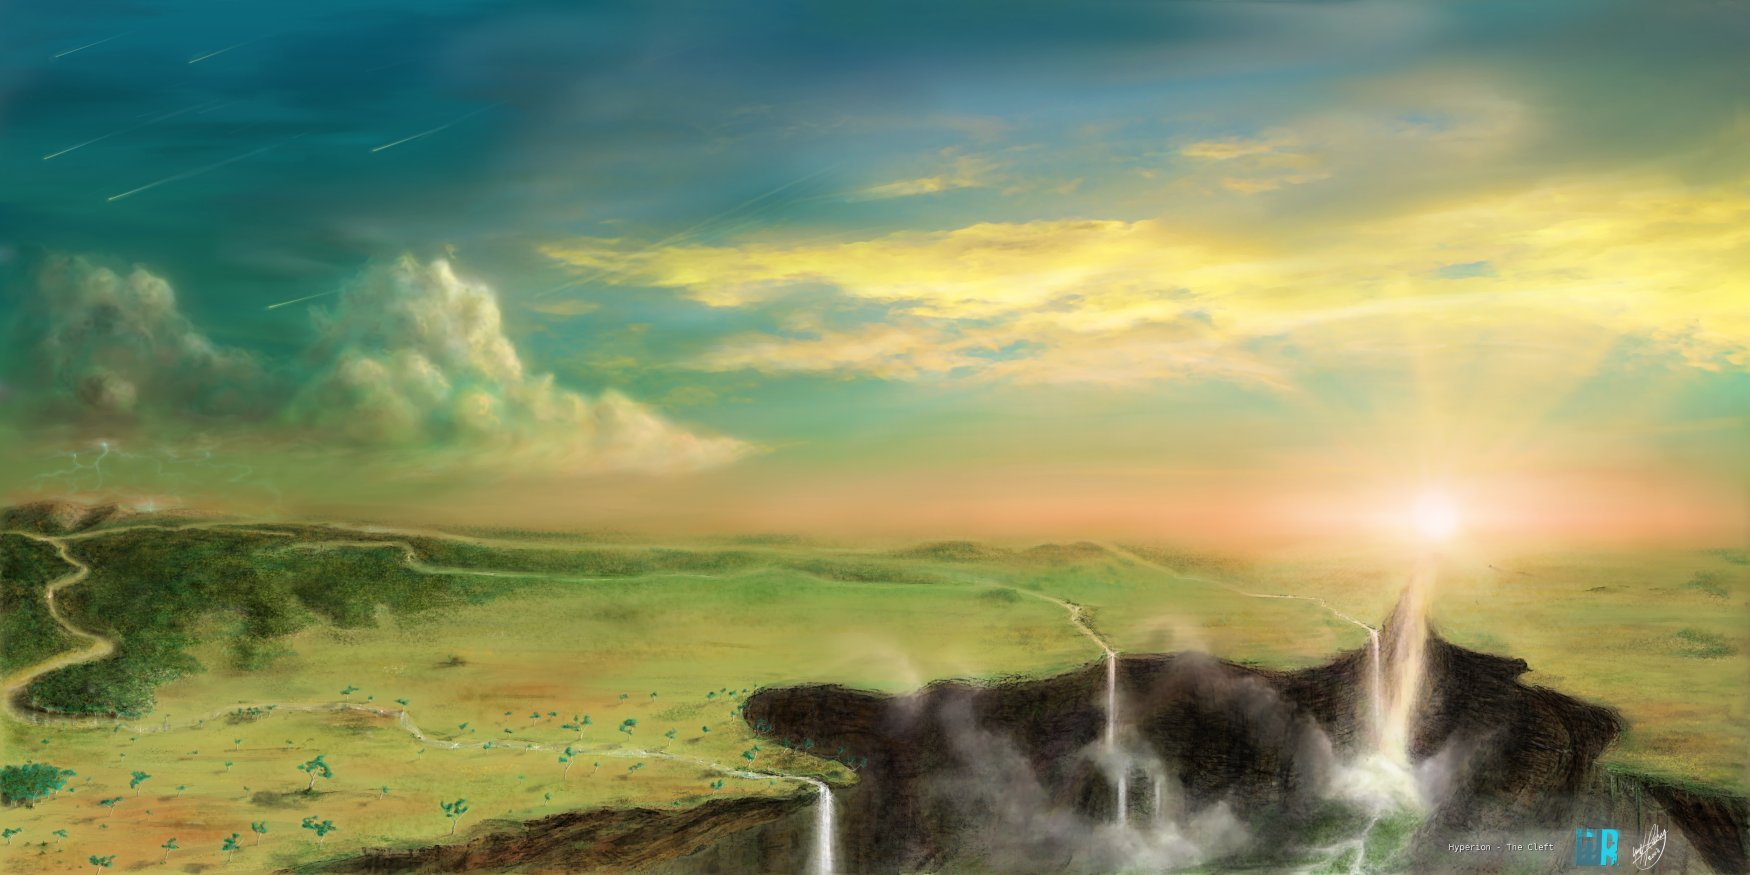
\includegraphics[width = 6cm]{takai.jpg}\\
\\
Il Takai possiede le seguenti caratteristiche:
\begin{itemize}
	\item Gravità normale
	\item Tempo normale
	\item Dimensioni Infinite
	\item Plasmabile divino
	\item Nessun elemento dominante
	\item Allineamento buono
	\item Magia normale
\end{itemize}

\subsection*{Fukai}
Il Fukai è il piano di origine delle creature infernali e abissali. È caratterizzato da un terreno di roccia di colore grigio spento, il quale è attraversato da numerose gallerie più o meno profonde. Inquietanti edifici fanno di queste gallerie le loro fondamenta.\\
\\
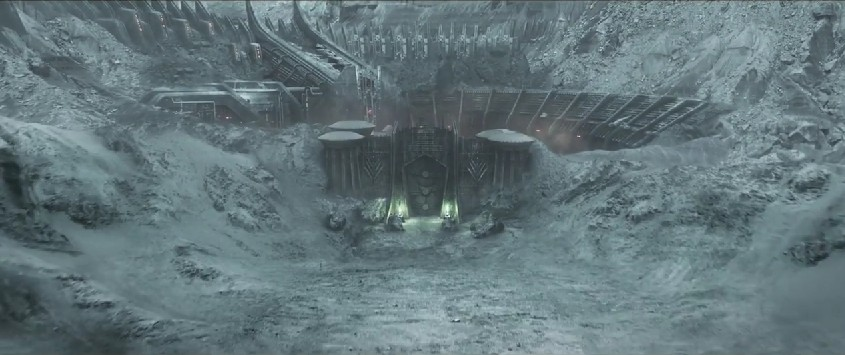
\includegraphics[width = 6cm]{fukai.jpeg}
\\
Il Fukai presenta i seguenti tratti:
\begin{itemize}
	\item Gravità normale
	\item Tempo normale
	\item Dimensioni Infinite
	\item Plasmabile divino
	\item Nessun elemento dominante
	\item Allineamento malvagio
	\item Magia normale
\end{itemize}

\end{multicols}

\chapter{Divinità}
\begin{multicols}{2}
\section{Introduzione}
In questo capitolo saranno descritti molto brevemente gli Dei principali, questi non sono gli unici che esistono, potreste entrare in contatto con culti rivolti a divinità minori o semi-divinità non riportate qui.
Faccio un piccolo cambiamento rispetto all'ambientazione canonica per quanto riguarda le divinità razziali: per quanto esse esistano sono anche associate ad altre cose e quindi non sono esclusive delle corrispettive razze. Tipicamente le divinità vivono nel Tatakai, in caso contrario sarà specificato diversamente.\\
Seguiranno delle tabelle per aiutare a grandi linee nella scelta della divinità da venerare \footnote{Nelle tabelle non compaiono tutte le divinità descritte}.\\
Se volete ruolare chierici o altre robe divine e volete una divinità custom o magari vi gira il cazzo perché non c'è la divinità della vostra razza possiamo trovare una soluzione, basta che lo diciate.

\section{Descrizione delle Divinità}
\subsection*{Althes}
Althes detto lo Sguardolesto, dio mezz'elfo della caccia, dei boschi e del tiro con l'arco, è di allineamento neutrale. Molti ranger, esploratori e mezz'elfi sono tra i suoi fedeli. I domini a lui associati sono Animal, Celerity e Viaggio, la sua arma prediletta è l'arco lungo composito.\\
\\
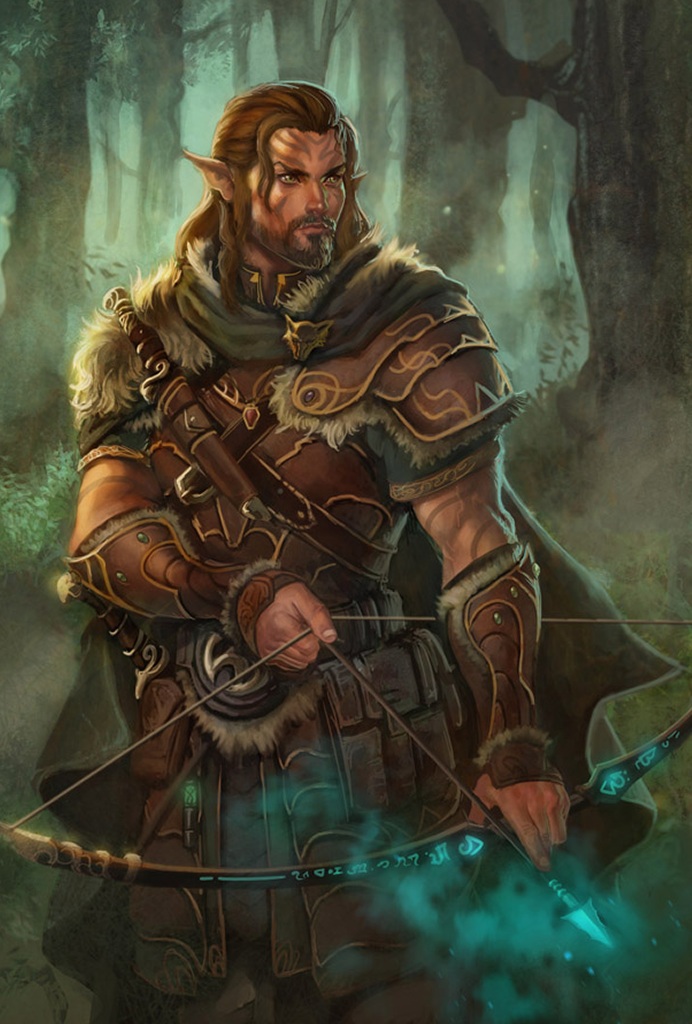
\includegraphics[width = 3.5cm]{althes.png}

\includegraphics[width = 4.5cm]{althes_simbolo.png}
\subsection*{As Vahal}
As Vahal, dio nanico della forgia, del fuoco e della metallurgia, è di allineamento legale neutrale. Egli è piuttosto brutto e di carattere volubile, ma con una grande forza nei muscoli delle braccia e delle spalle, e dotato una tale abilità artigiana per cui tutto ciò che crea è di un'impareggiabile perfezione. I nani, i fabbri e gli artigiani sono i suoi fedeli. Ha dimora nel Tatakai ma passa più tempo nella sua Grande Fucina situata sul Titano del Fuoco. I domini a lui associati sono Fuoco, Craft e Forza, mentre la sua arma è il martello da guerra.\\
\\
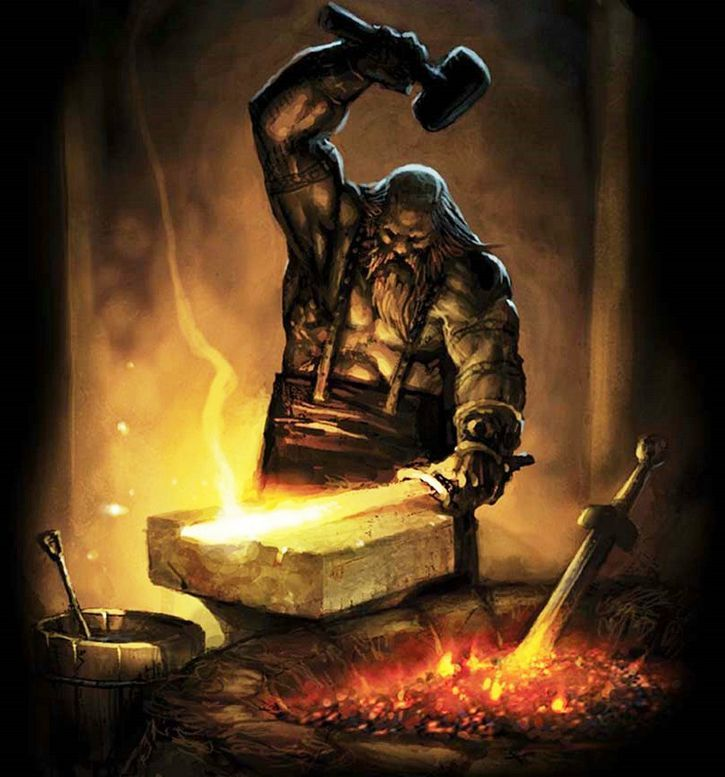
\includegraphics[width = 3.5cm]{asvahal.jpg}
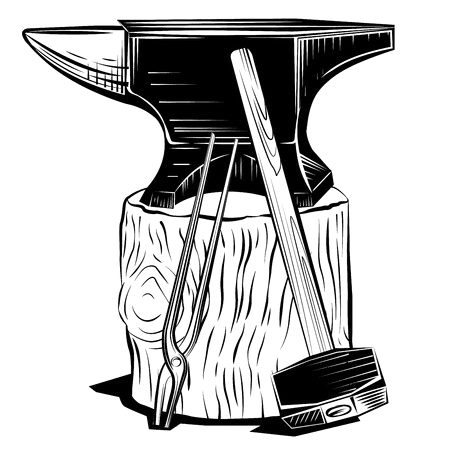
\includegraphics[width = 3cm]{asvahal_simbolo.jpg}
\subsection*{Bhar B'Hero}
Bhar B'Hero è il dio elfico della conoscenza, della storia e della filosofia, di allineamento neutrale. Il suo titolo è Il Sapiente, viene rappresentato come un vecchio elfo. Scolari, studiosi, eruditi, maghi, bardi sono spesso suoi fedeli, ai quali si aggiungono elfi e mezzelfi. I domini a cui è associato sono Conoscenza, Guarigione e Magia. La sua arma preferita è il bastone ferrato.\\
\\
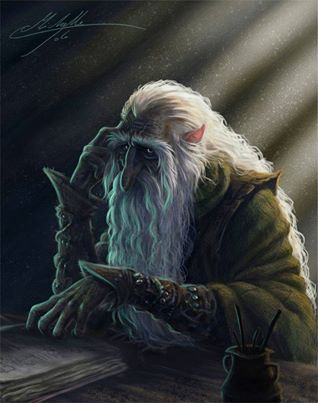
\includegraphics[width=3.5cm]{bharbhero.jpg}

\includegraphics[width=3cm]{bharbhero_symbol.png}
\subsection*{Byrœ}
Byrœ è il dio dell'arte, della musica, della poesia e dello spettacolo, di allineamento caotico neutrale. Egli è il protettore dei bardi e bardo egli stesso, ama la musica, le feste e le donne. È venerato principalmente da bardi e artisti ma talvolta anche dai ladri più festaioli. Egli vive nel Tatakai ma passa la maggior parte del suo tempo nel Piano Materiale. I suoi domini sono Joy, Viaggio e Charm. La sua arma preferita è lo stocco.\\
\\
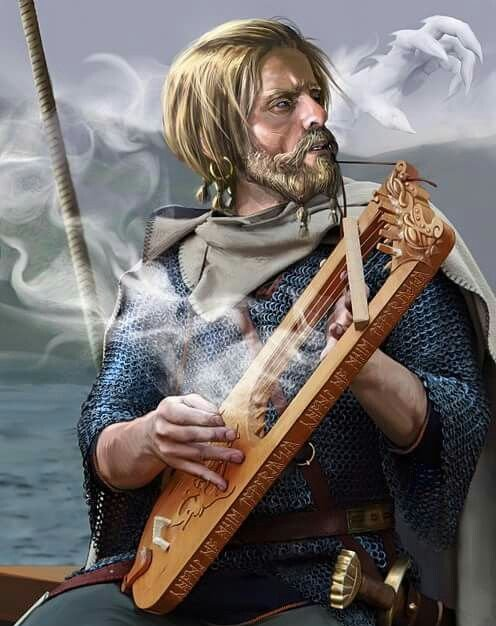
\includegraphics[width=3.5cm]{byroe.jpeg}
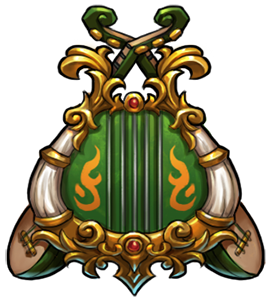
\includegraphics[width=3cm]{byroe_simbolo.png}
\subsection*{Cha Ah'ad}
Cha Ah'ad è il dio della forza, della prestanza fisica, protettore degli atleti e delle abitudini sane. È di allineamento legale neutrale, predilige l'attività fisica e l'allenamento allo studio e l'eruditismo. I suoi seguaci sono spesso guerrieri, monaci e paladini, e in generale atleti. I suoi titoli sono Pugno Empireo e Pugile del Tatakai. I suoi domini sono Forza, Pride, Competition e Glory. La sua arma preferita è il colpo senz'armi. I chierici di Cha Ah'ad ottengono Colpo Senz'Armi Migliorato come talento bonus.\\
\\
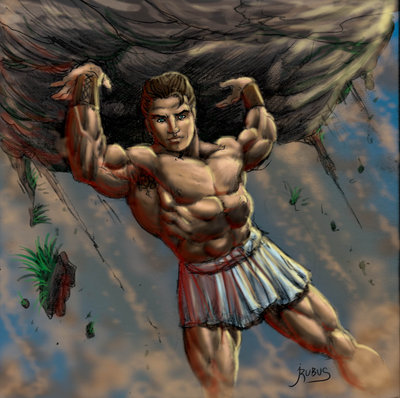
\includegraphics[width=4cm]{chaahad.jpeg}
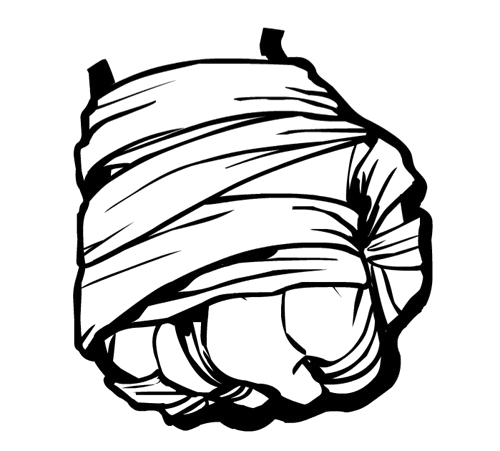
\includegraphics[width=3cm]{chaahad_simbolo.png}
\subsection*{Cloit, Claef e Cleos}
Cloit, Claef e Cleos sono i tre cavalieri di Kygeus. Cloit è legale neutro e rappresenta il giudizio e il castigo, simboleggiato dalla spada della giustizia di Kygeus. Claef (femminile) è di allineamento neutrale buono e simboleggia lo splendore e il valore, rappresentati dai raggi del sole. Cleos è neutrale e è il simbolo del coraggio e della forza, e viene rappresentato dal leone. I tre cavalieri solitamente sono riconosciuti come divinità minori e complementari a Kygeus stesso, ma alcune declinazioni della chiesa di Kygeus le considera un'entintà unica da venerare separatamente. I domini sono: Legge per Cloit, Nobility per Claef e Courage per Cleos. La loro arma preferita è la spada lunga.\\
\\
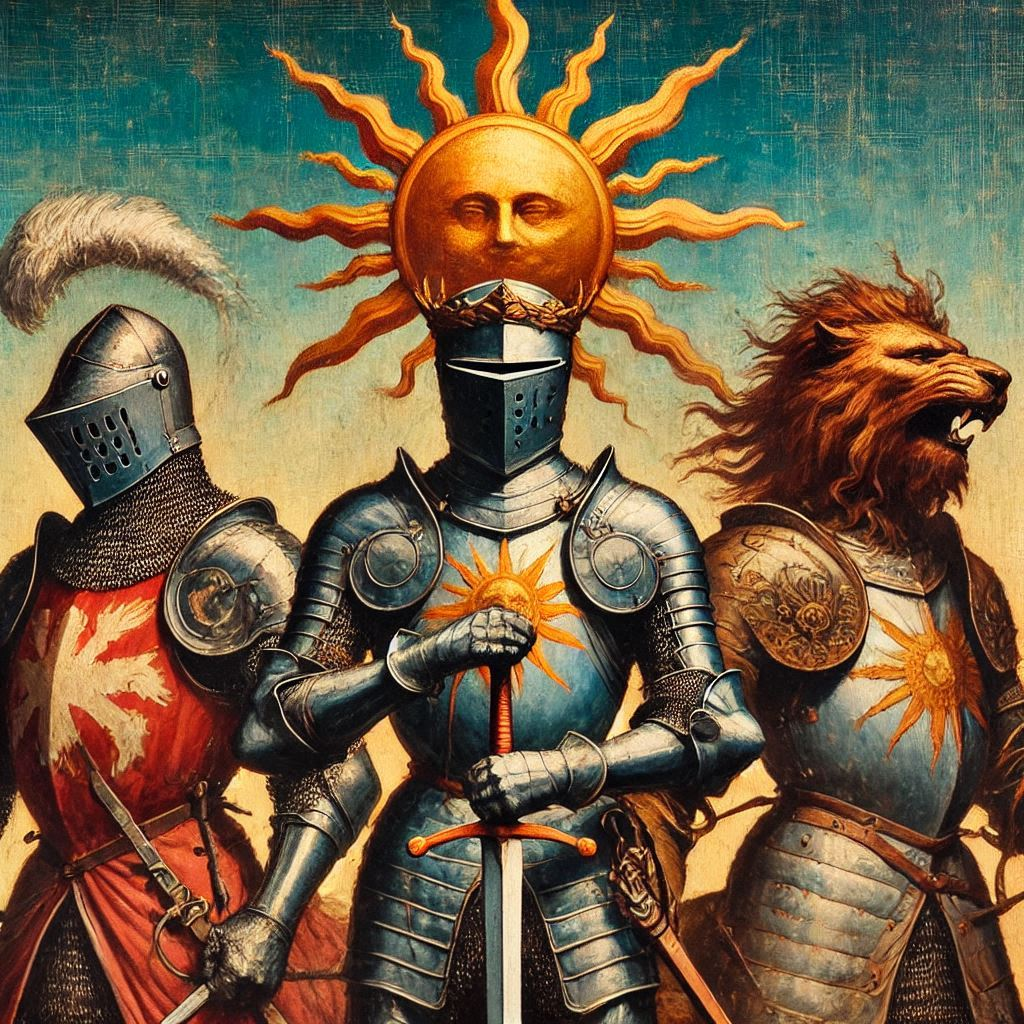
\includegraphics[width=4cm]{ccc.jpeg}

\includegraphics[width=4cm]{ccc_simbolo.png}
\subsection*{Coepius}
Dio dell'agricoltura, del sole e dell'abbondanza, Coepius è neutrale buono. Chiamato anche Il Benefattore egli è venerato dai contadini che pregano per un'abbondante raccolto e dai personaggi buoni. I domini a lui associati sono Sole, Bene e Guarigione. La sua arma è il falcetto.\\
\\

\includegraphics[width=3.5cm]{coepius.jpg}
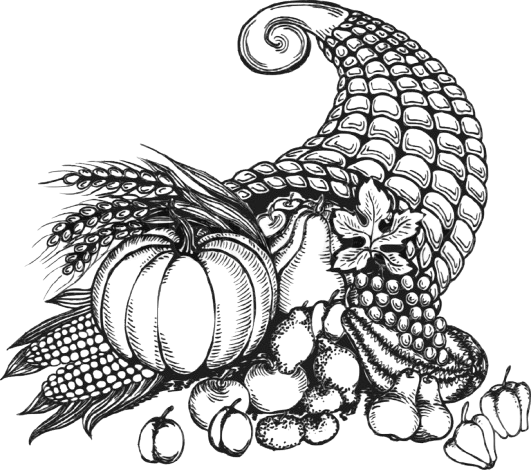
\includegraphics[width=3.5cm]{coepius_simbolo.png}
\subsection*{Dictum}
Dictum è il dio della morte e della resurrezione, è legale neutrale. Conosciuto con il nome di Eterno Scrittore, si dice che possegga un'infinita pergamena su cui scrive i nomi di chi muore e cancella quelli di chi viene resuscitato. I suoi chierici si occupano di funerali e dei riti durante il festival delle Anime Perdute. I suoi domini sono Morte, Repose e Legge. La sua arma è il mazzafrusto pesante.\\
\\
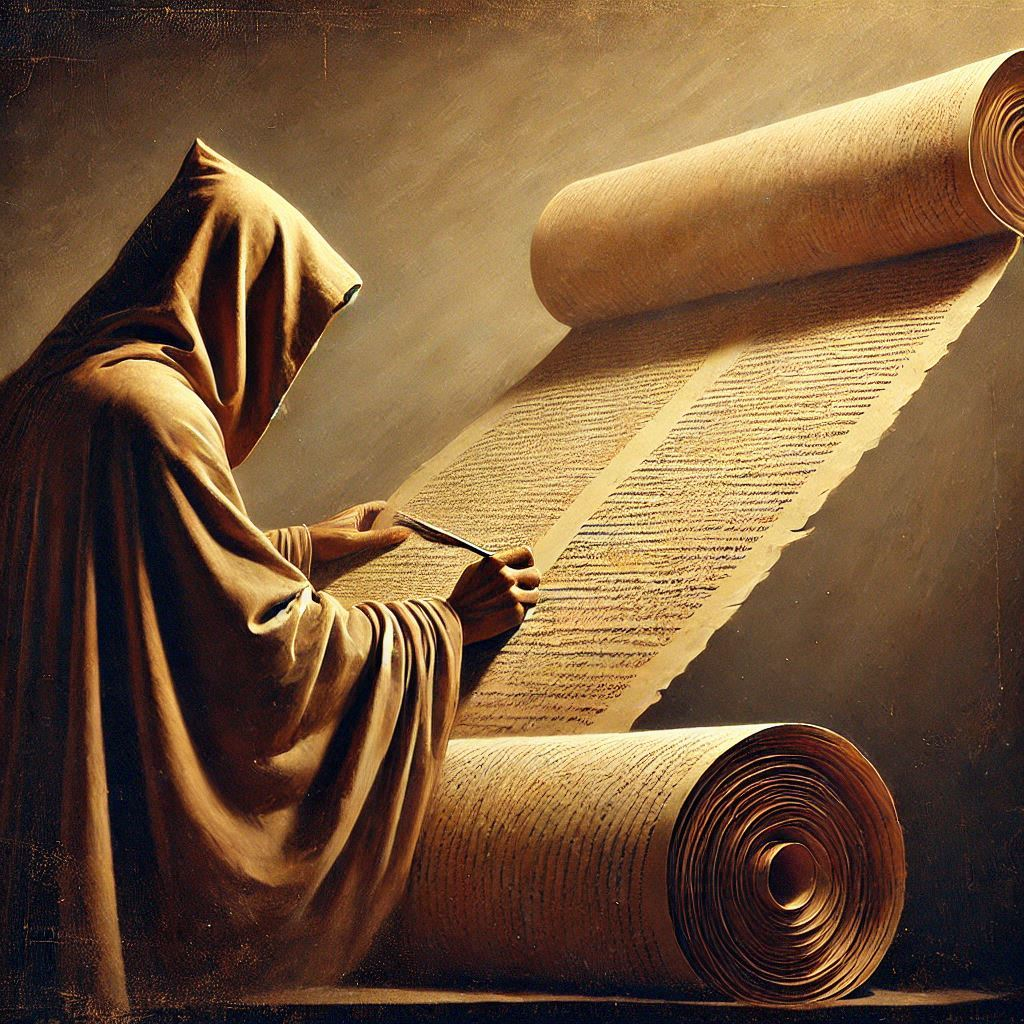
\includegraphics[width=3.5cm]{dictum.jpeg}
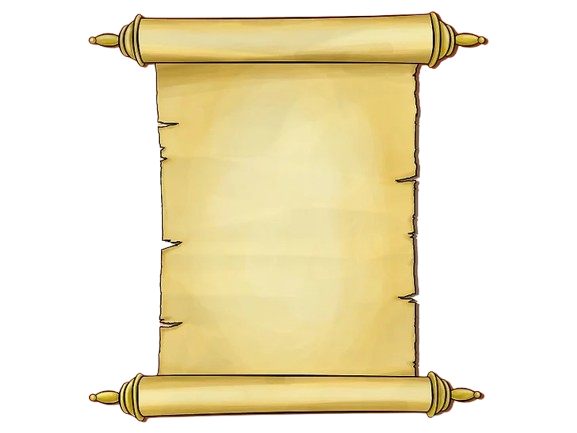
\includegraphics[width=3.5cm]{dictum_simbolo.png}
\subsection*{Djenl}
Djenl è la dea halfling della gioia, dell'ottimismo e della prudenza come via per la serenità. È di allineamento neutrale buono. La protettrice degli halfling è venerata anche da individui di altre razze che prediligono la previdenza all'avventatezza. Viene chiamata anche Colei-che-sorride-al-domani e Custode del Cuor Leggero. I suoi domini sono Protezione, Planning, e Joy. La sua arma preferita è la scimitarra.\\
\\
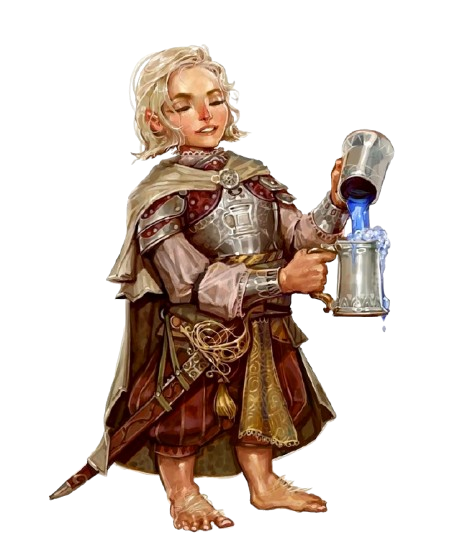
\includegraphics[width=4cm]{djenl.png}

\includegraphics[width=3cm]{djenl_simbolo.jpeg}
\subsection*{Fjorsh}
Fjorsh il Solitario, dio mezzorco della solitudine, del conflitto interiore, della redenzione e della perseveranza, è di allineamento neutrale buono. Tra i suoi fedeli ci sono mezzorchi che si sentono rifiutati da entrambe le loro origini, guerrieri solitari che vagano senza un posto a cui appartenere, eremiti, viandanti, anime spezzate che cercano redenzione o che lottano con il dolore della perdita e del rifiuto, e chiunque senta di portare un peso che gli altri non possono comprendere. Fjorsh vaga solitario per i piani, tuttavia, il suo isolamento è fonte di forza: attraverso il dolore della solitudine, insegna ai suoi seguaci a trovare potere nella resilienza e a cercare un senso di pace interiore. Alcuni monaci decidono di seguire le sue orme spirituali. I suoi domini sono Endurance, Viaggio e Mind mentre la sua arma prediletta è l'ascia da battaglia.\\
\\
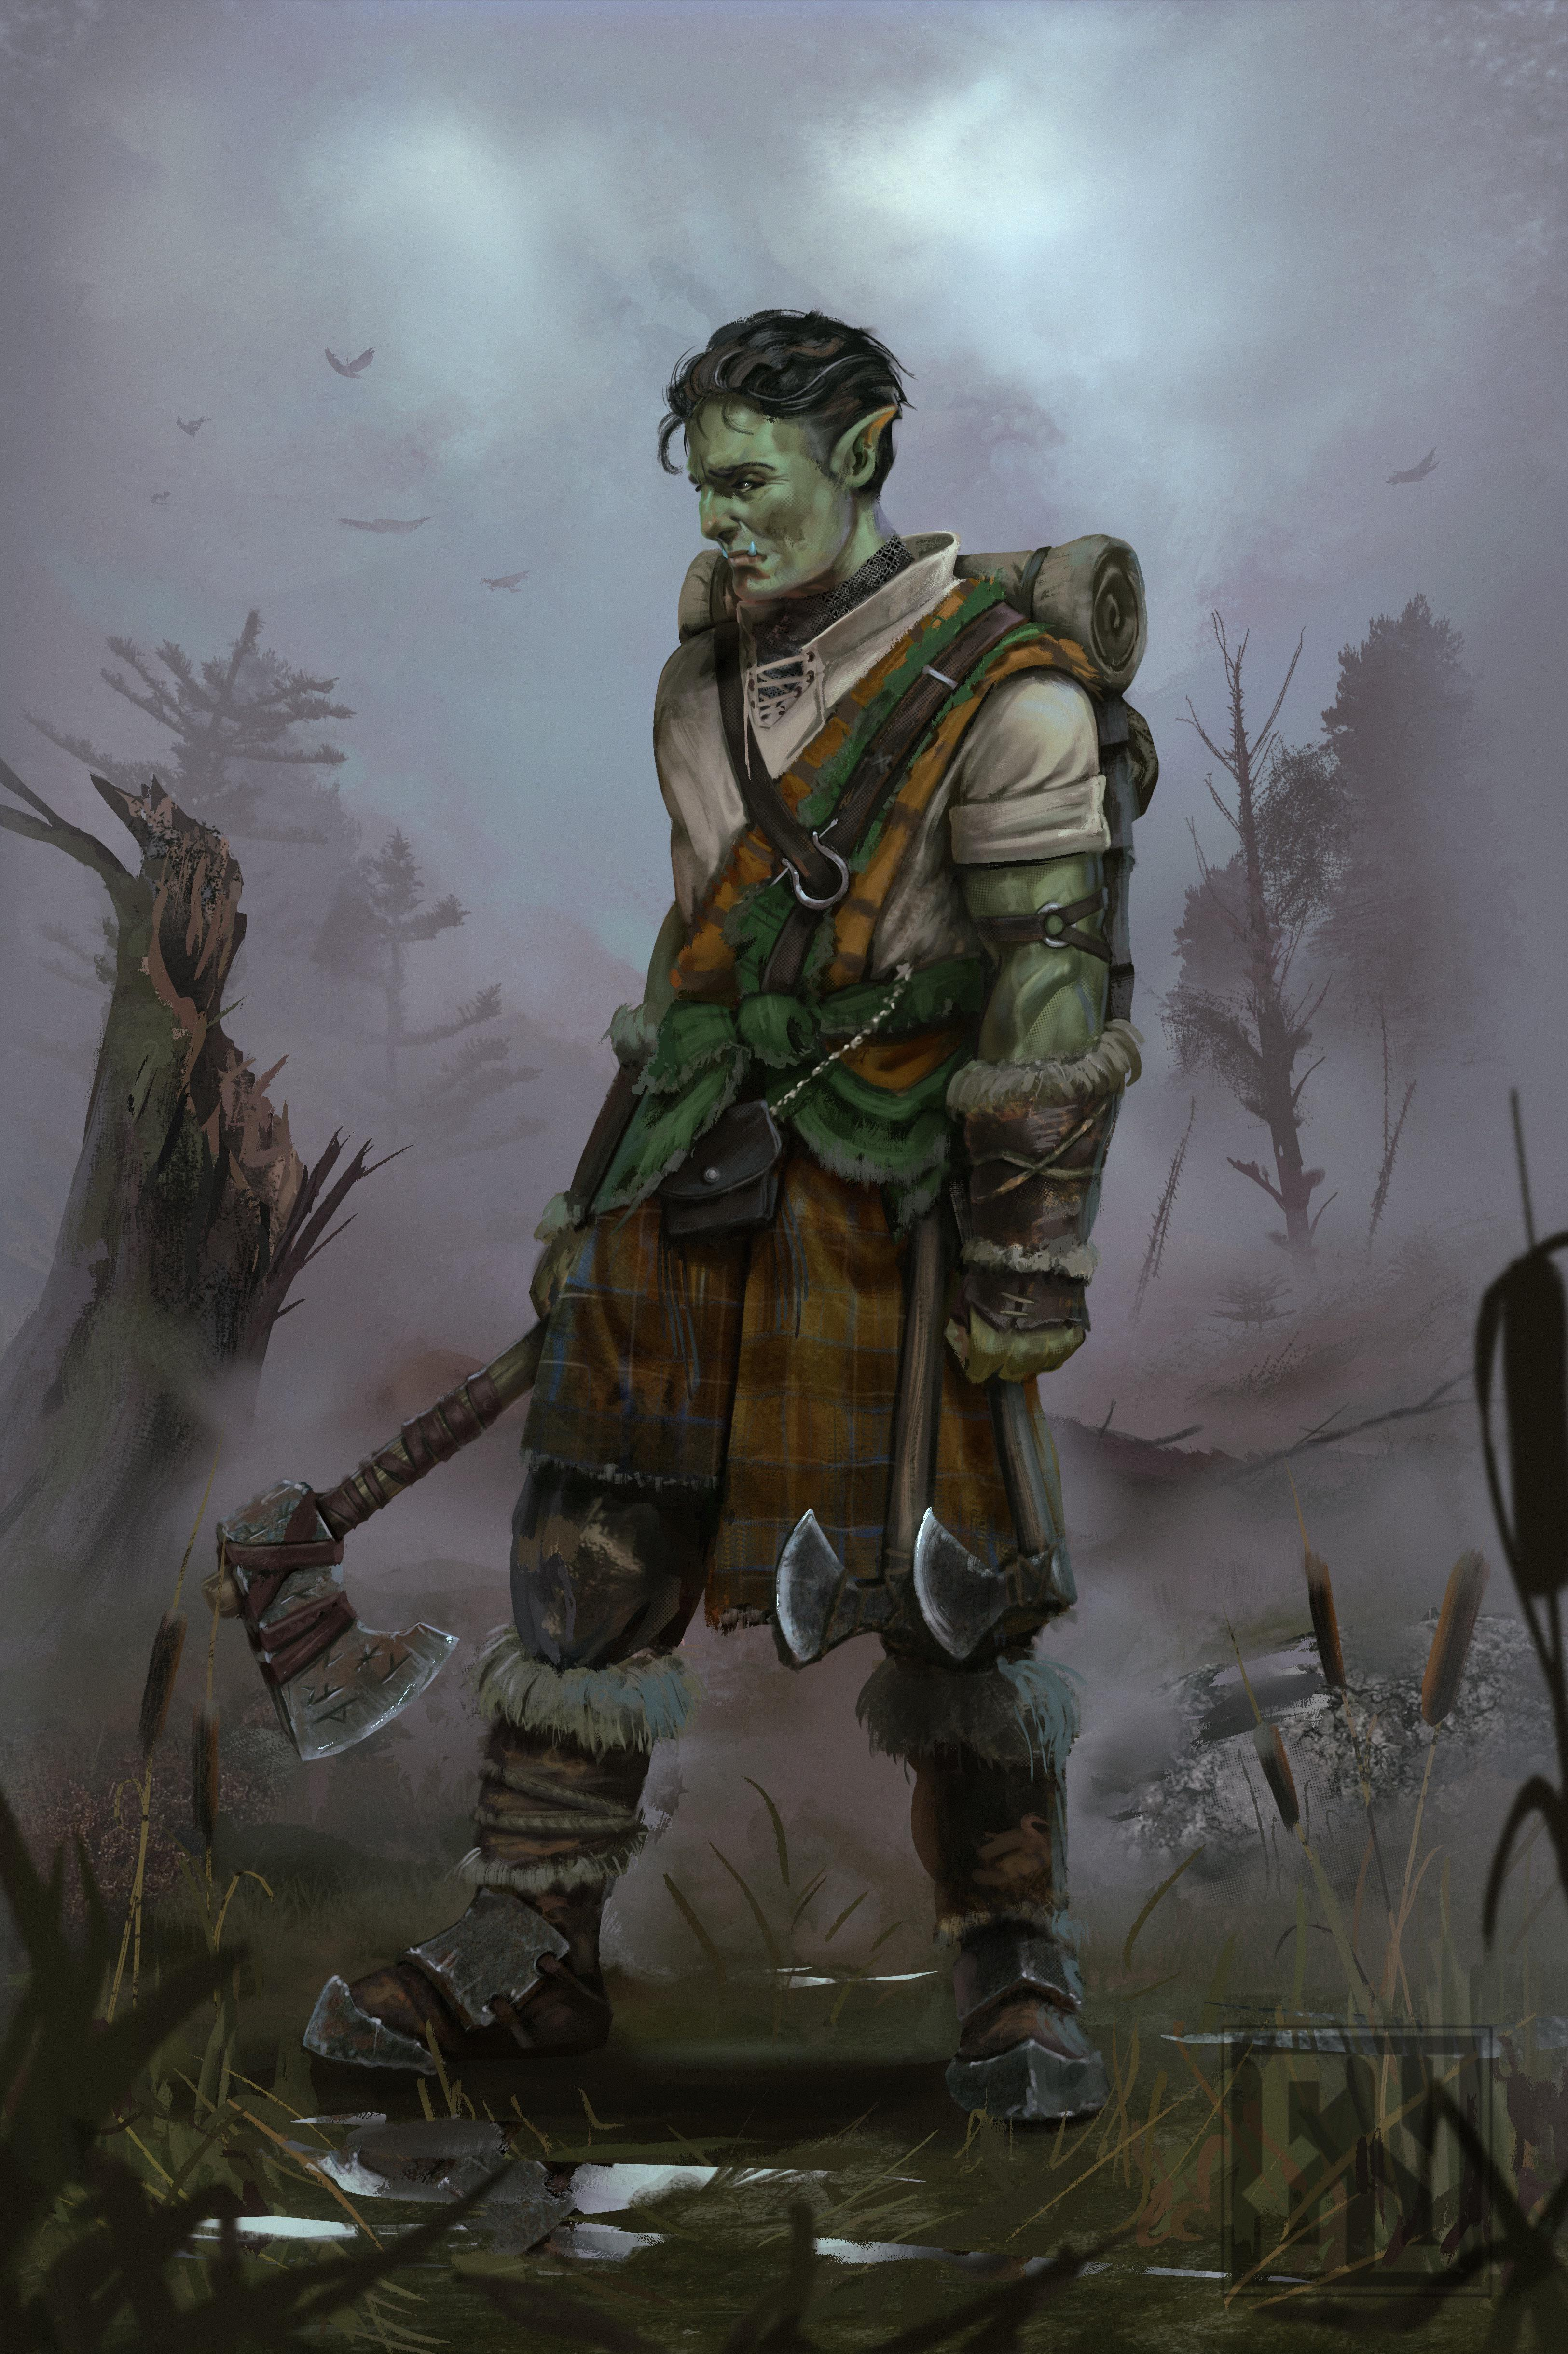
\includegraphics[width = 3.5cm]{fjorsh.jpg}
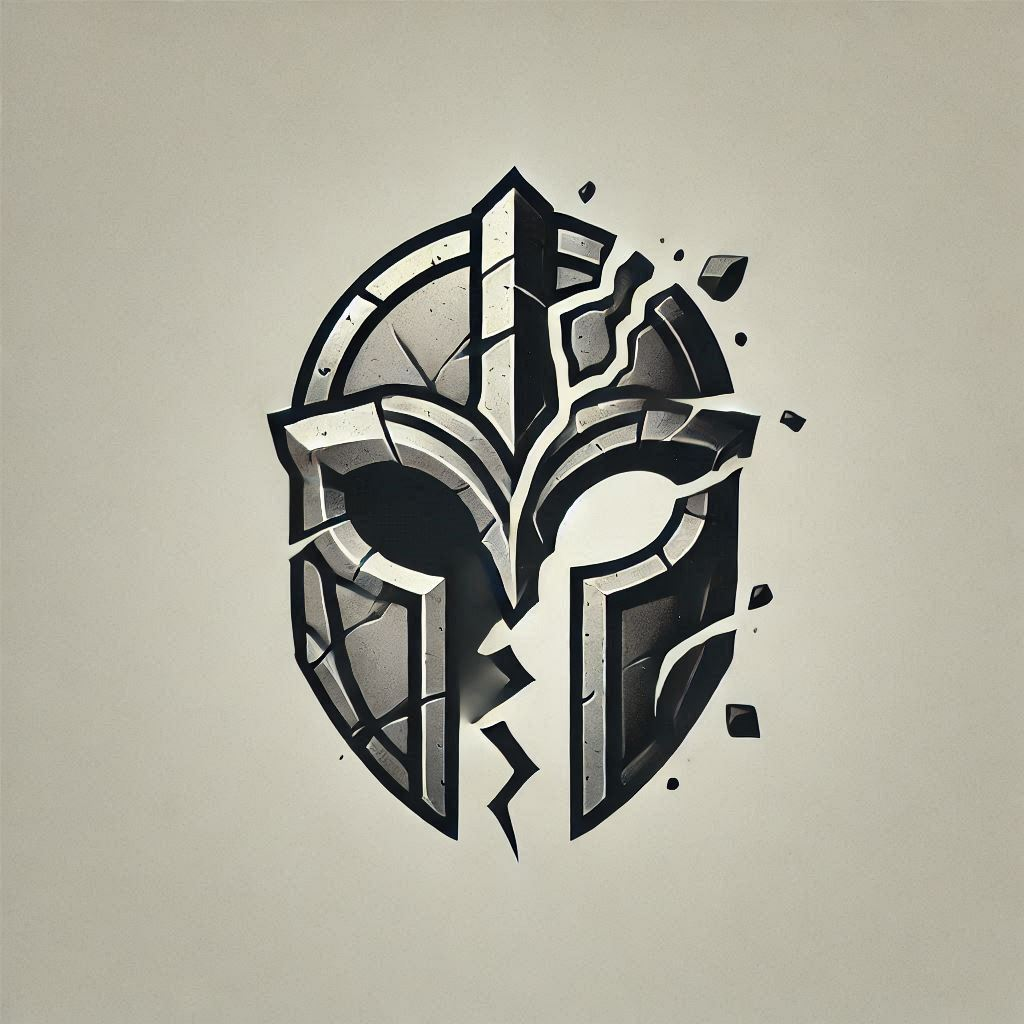
\includegraphics[width = 3.5cm]{fjorsh_simbolo.jpeg}\\
\subsection*{Hnana}
Hnana, dea della natura, protettrice degli animali e delle piante è di allineamento neutrale buono. Viene raffigurata come una ninfa e è conosciuta come La Pacifica. Spesso è venerata da folletti, gnomi, halfling ed elfi. Anche ranger e druidi sono tra i suoi seguaci. Nonostante viva nel Tatakai, Hnana passa molto tempo sui Titani elementali (Aria, Acqua, Terra, Fuoco). \\
I suoi domini sono Animale, Vegetale, Acqua, Fuoco, Terra e Aria, mentre la sua arma prescelta è la lancia.\\
\\
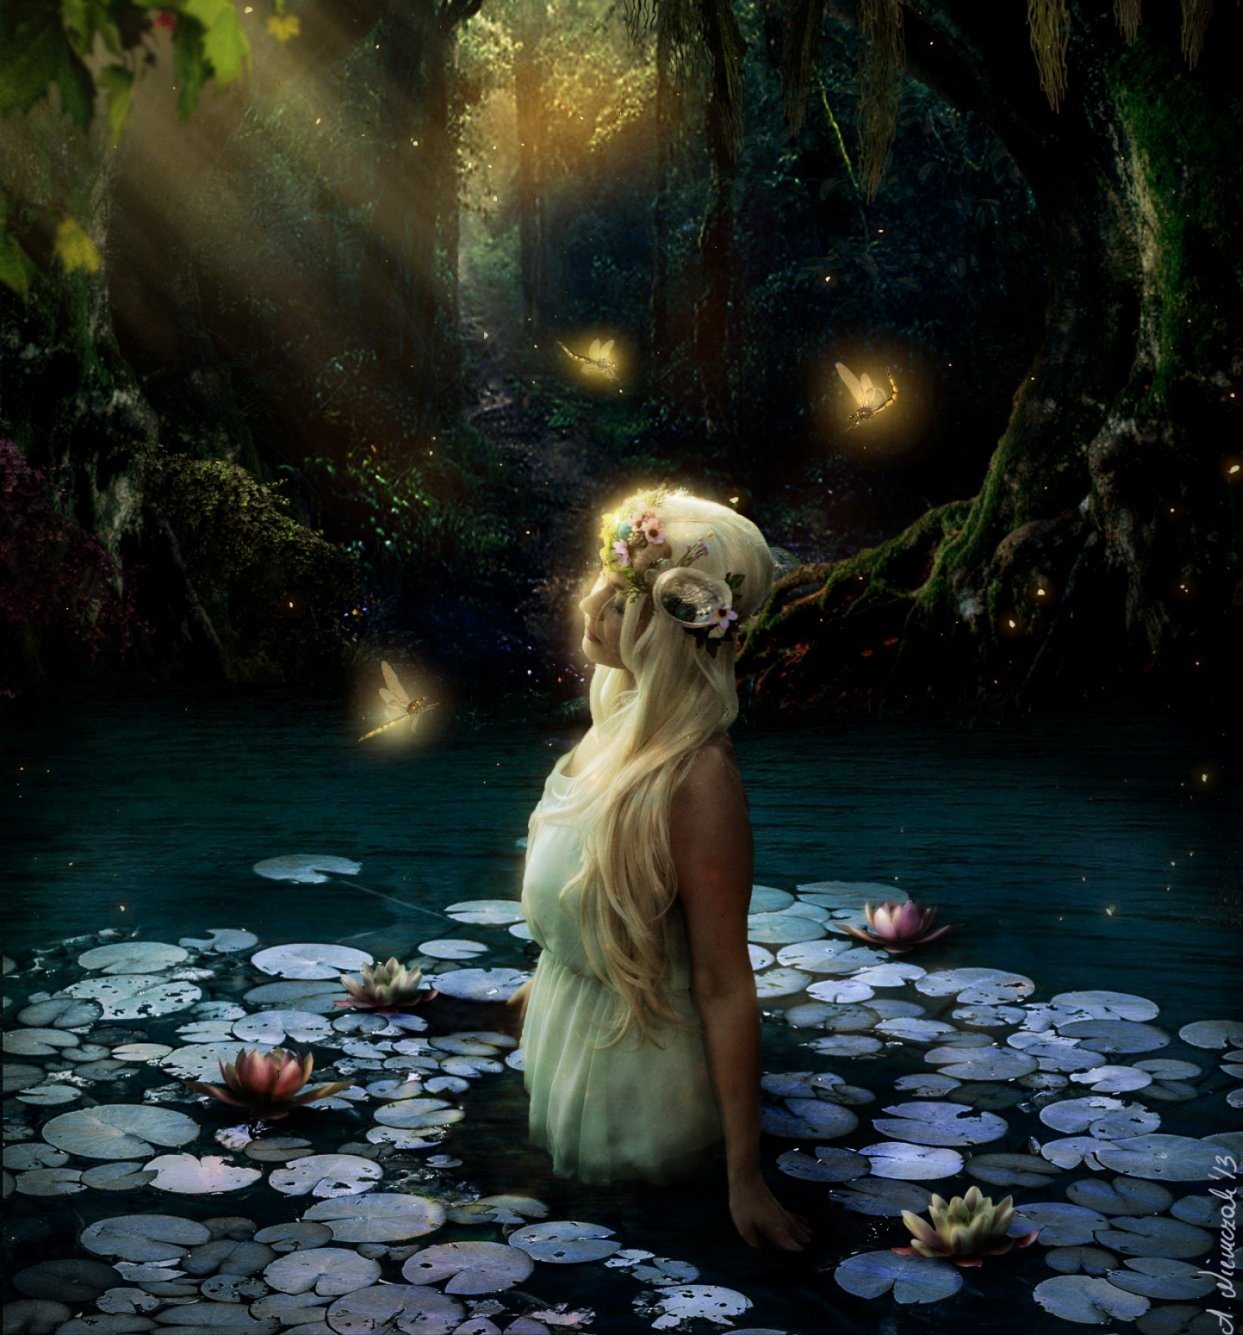
\includegraphics[width = 4cm]{hnana.jpeg}
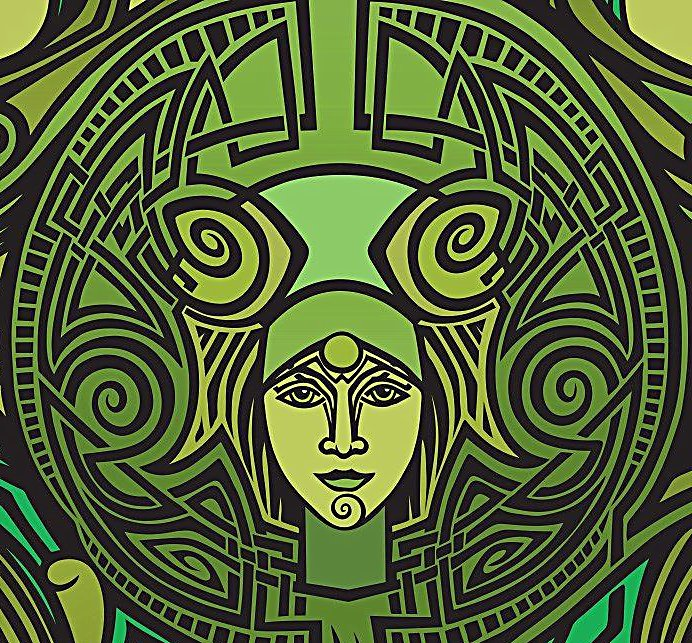
\includegraphics[width = 3cm]{hnana_simbolo.jpeg}\\
\subsection*{Huaifu}
Huaifu è la dea della bellezza, dell'amore e dell'affetto, di allineamento caotico buono. È la protettrice degli innamorati, dei matrimoni e della famiglia, viene raffigurata come una dama di ineguagliabile bellezza. Si dice che la sua bellezza sia la causa dell'invidia e della pazzia della sorella Tahia. I suoi seguaci sono principalmente bardi. I suoi domini sono Lust, Protezione, Bene e Community, mentre la sua arma preferita è la spada corta.\\
\\
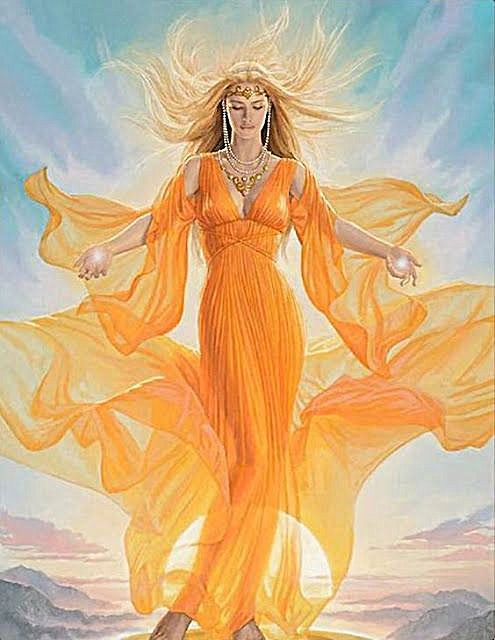
\includegraphics[width=3.5cm]{huaifu.jpeg}

\includegraphics[width=4cm]{huaifu_simbolo.png}
\subsection*{Immaru}
Immaru il Terribile, dio della paura, del tormento e della tortura è di allineamento legale malvagio. È il protettore di coloro che infliggono dolore e sofferenza. I suoi fedeli sono principalmente guerrieri, paladini e monaci malvagi. Per la sua malvagità Immaru è stato cacciato dal Tatakai; vive dunque nel Fukai. I suoi domini sono Male, Legge, Forza e Guerra mentre la sua arma prediletta è la catena chiodata.\\
\\
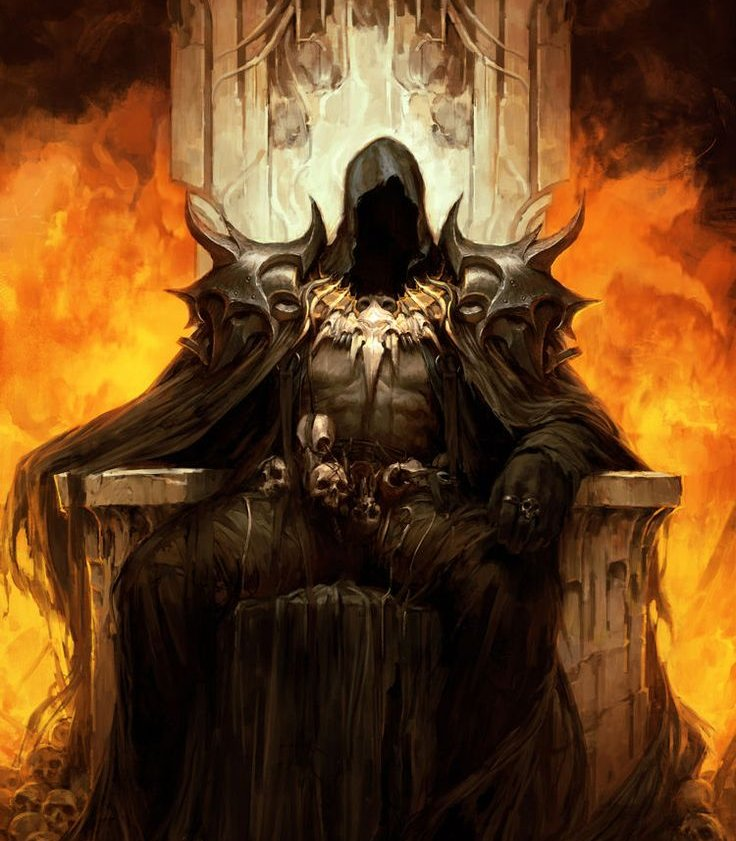
\includegraphics[width = 3.5cm]{immaru.jpg}

\includegraphics[width = 3cm]{immaru_simbolo.jpg}\\
\subsection*{Kygeus}
Il dio della guerra, del valore e della giustizia, Kygeus è legale buono. Chiamato anche Spada della Legge è venerato da guerrieri, paladini e monaci.
Protegge i deboli e punisce chi commette ingiustizie. 
I domini a cui è associato sono Bene, Guerra, Coraggio, Legge e Forza, la sua arma preferita è lo spadone.\\
\\
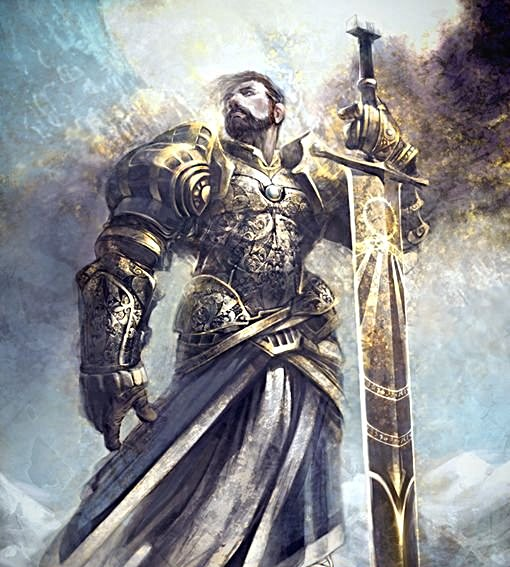
\includegraphics[width = 3.5cm]{kygeus.jpeg}
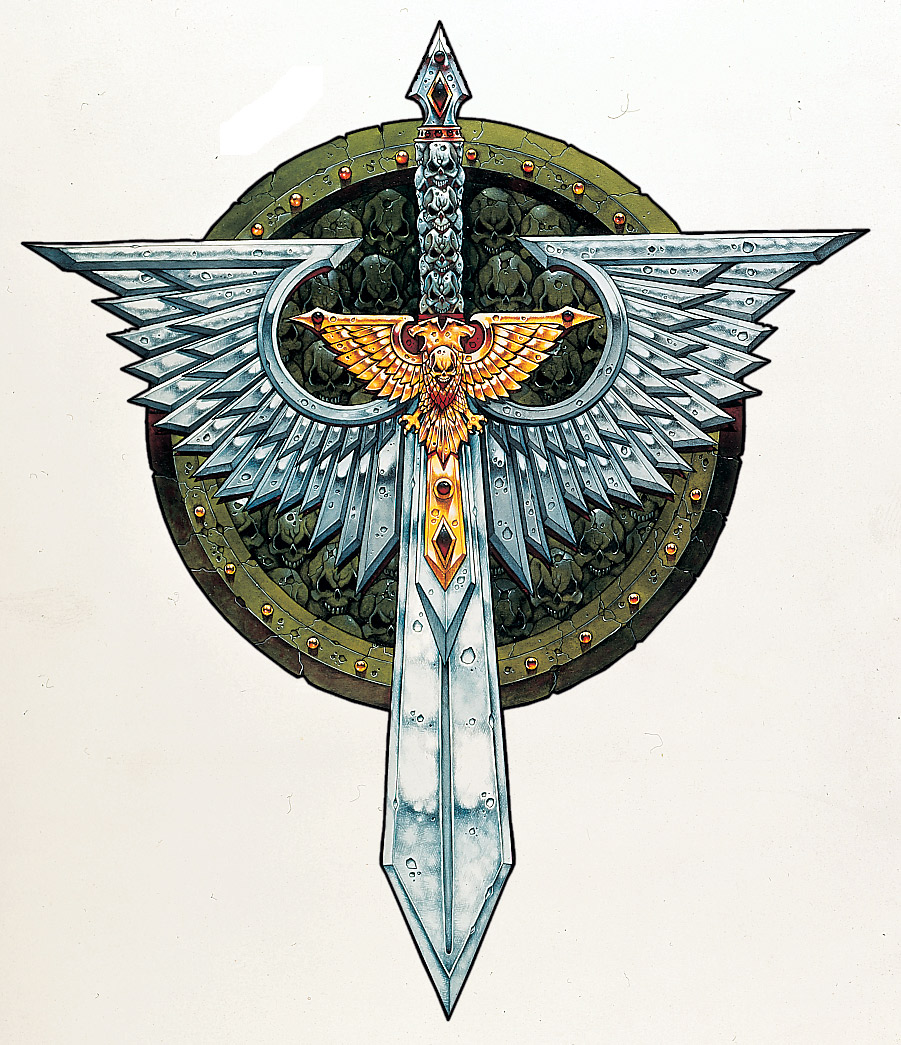
\includegraphics[width = 3cm]{kygeus_simbolo.jpg}
\subsection*{Lialgha}
La dea della morte Lialgha è di allineamento neutrale malvagio. Tra i suoi titoli ci sono: La Fredda Morsa e Dama della Morte. Appare come una pallida dama vestita di bianco. I suoi fedeli sono principalmente ladri malvagi, creature malvagie e negromanti ma spesso anche stregoni e maghi malvagi.\\
Preferisce vivere sul Titano dell'Energia Negativa ma non è bandita dal Tatakai. I suoi domini sono Morte, Male e Magia mentre la sua arma è il pugnale.
\\
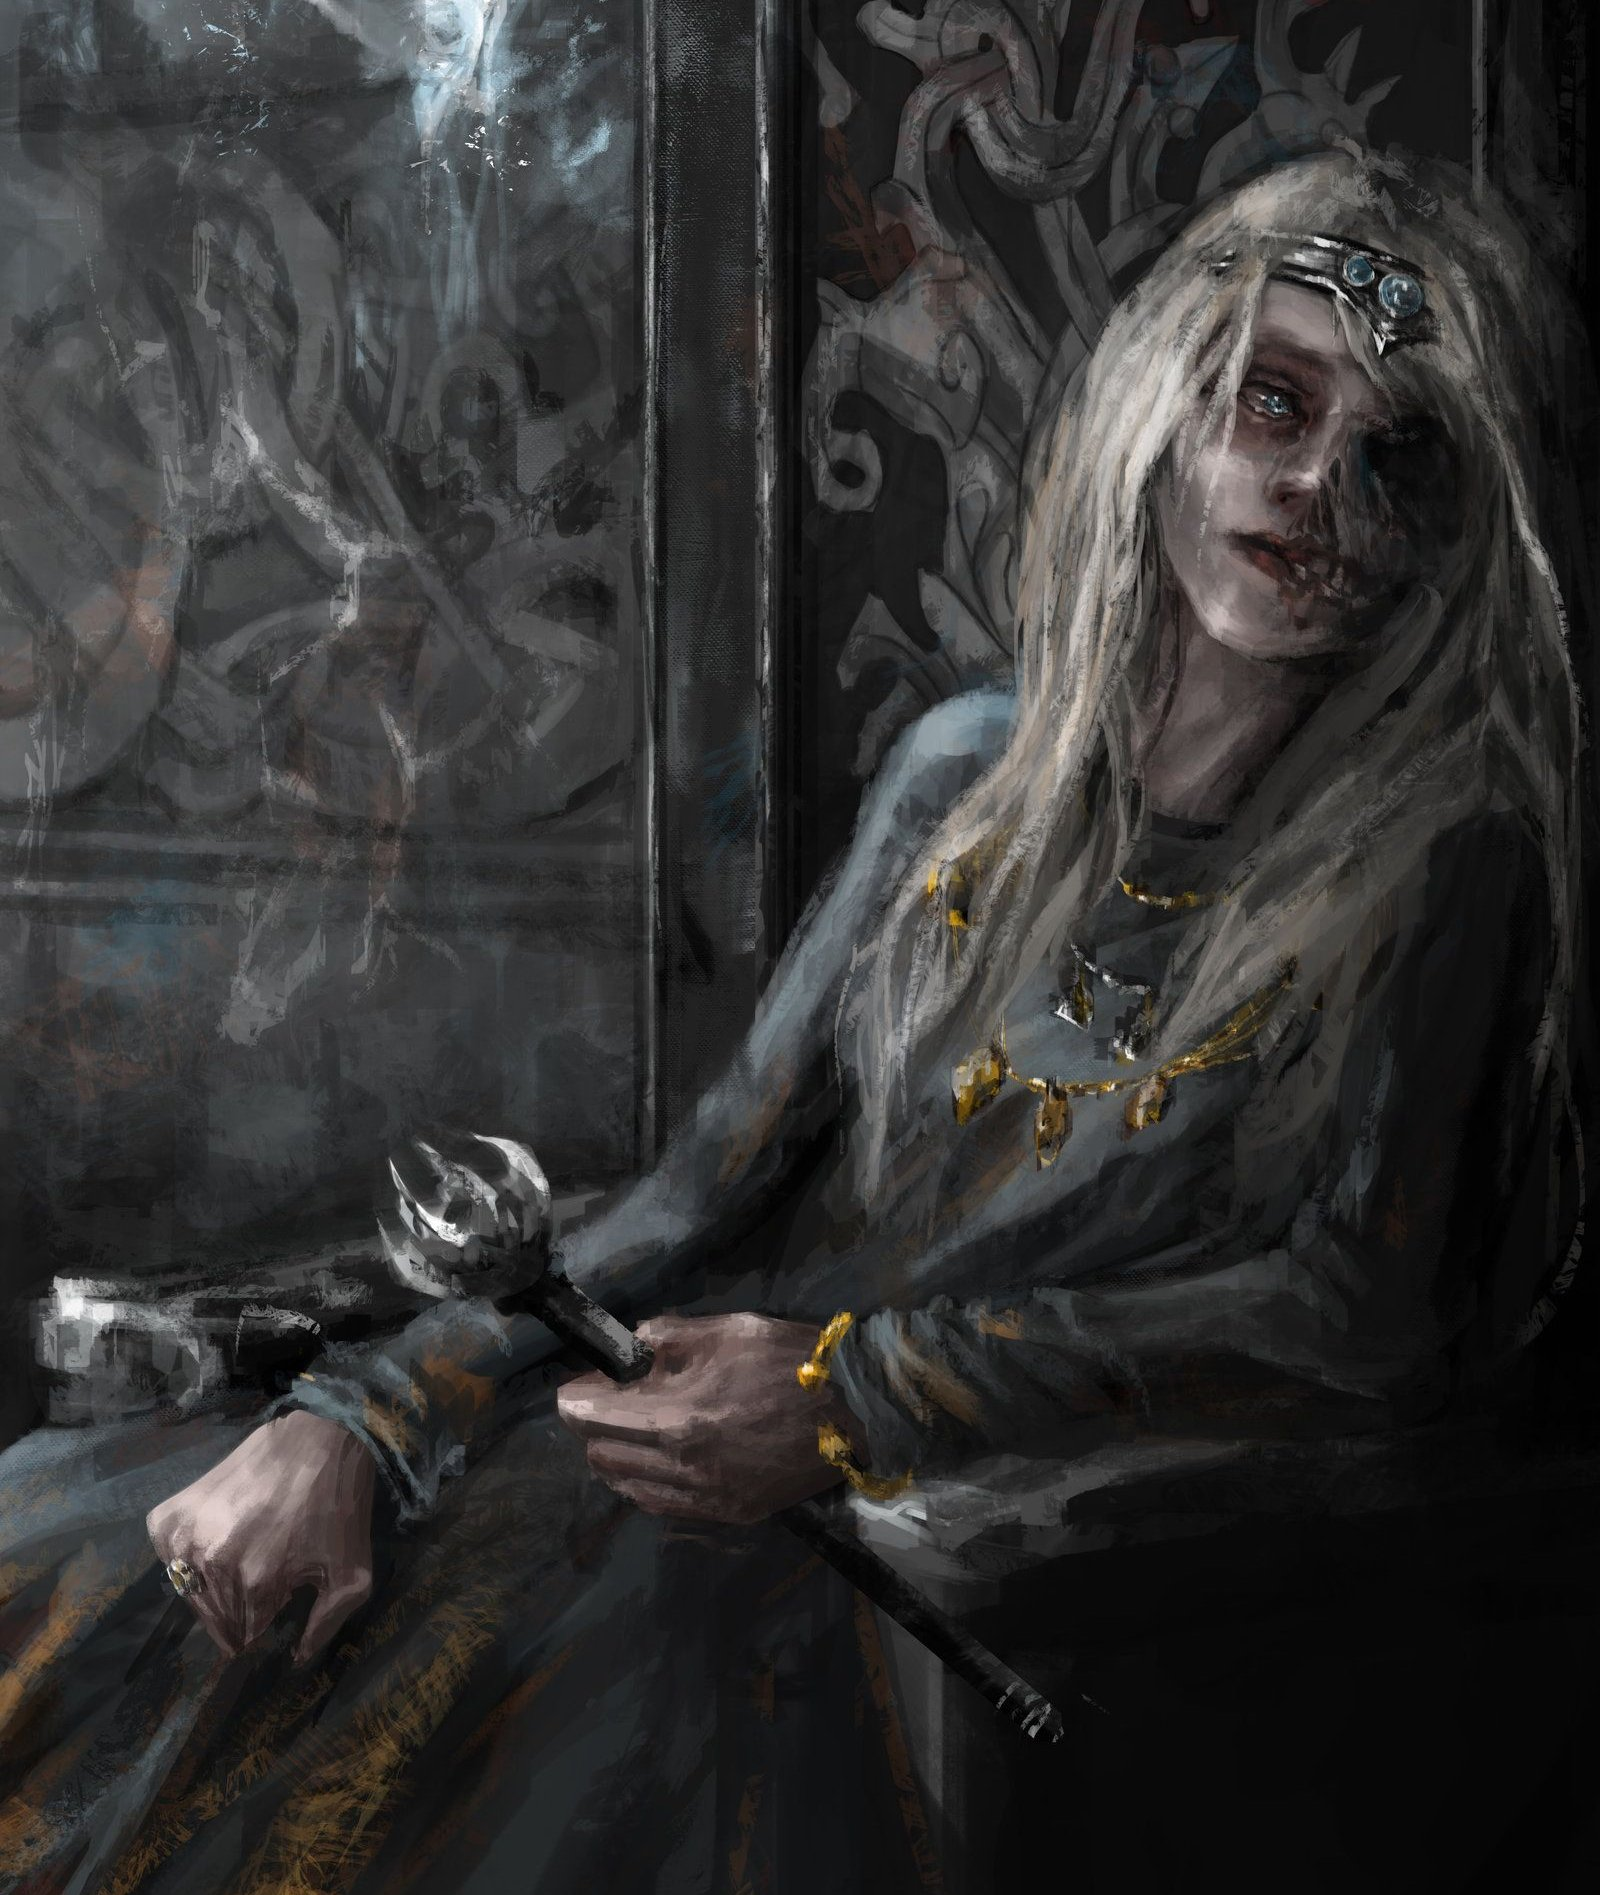
\includegraphics[width=3.5cm]{lialgha.jpeg}
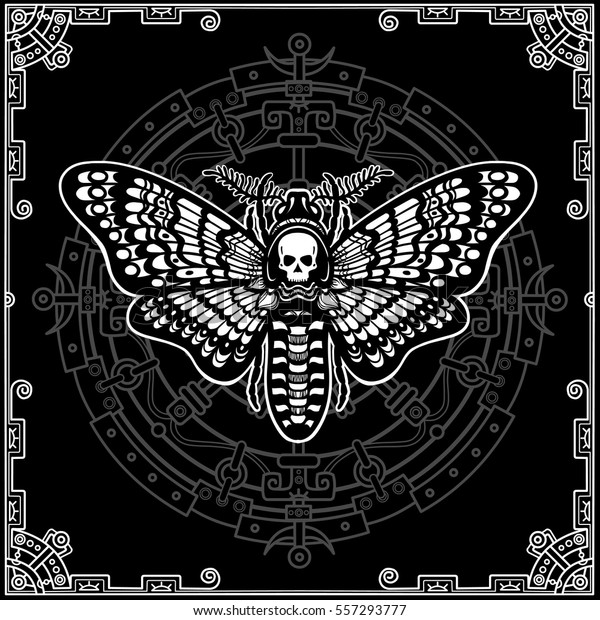
\includegraphics[width=3cm]{lialgha_simbolo.jpeg}
\subsection*{Moohona}
La dea della magia, Moohona, è neutrale. La sua grande conoscenza è superata solo dal grande Bhar B'Hero. I suoi titoli sono Maga Celeste e Madre di Scintipietra. I suoi fedeli sono principalmente maghi e stregoni ma occasionalmente anche bardi. Nonostante abbia dimora nel Tatakai passa la maggior parte del suo tempo nel Mare di Stelle. I suoi domini sono Magia, Conoscenza, Oracle e Spell. La sua arma preferita è il bastone ferrato.\\
\\
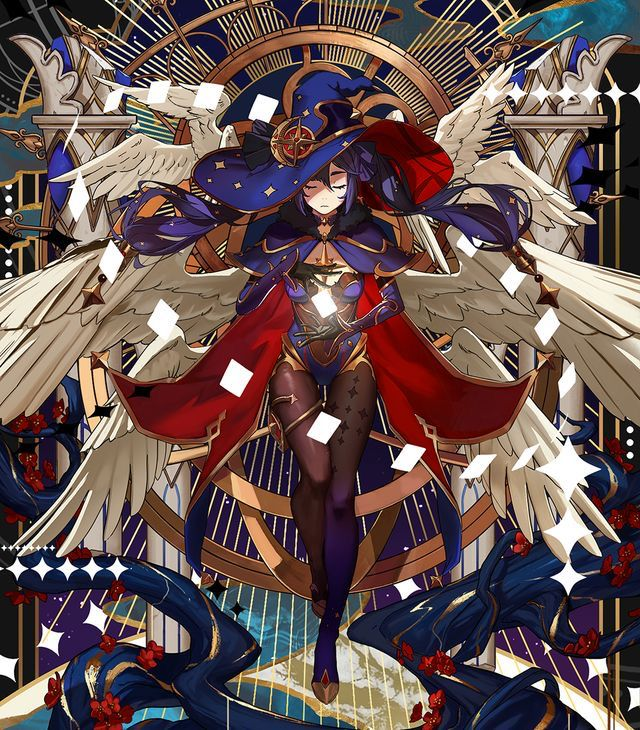
\includegraphics[width=4cm]{mona1.jpeg}
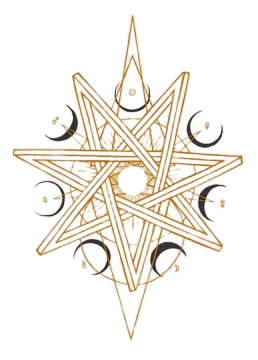
\includegraphics[width=3cm]{moohona_simbolo.jpg}
\subsection*{Pathon}
Pathon, dio della fortuna e dei tesori nascosti è di allineamento caotico neutrale. Il suo titolo è Il Dio Pigro, perché ottiene ciò che vuole con la fortuna e non con il lavoro, e viene quindi venerato da quegli avventurieri che desiderano tesori e ricchezze senza la fatica di combattere, principalmente ladri e bardi. I domini a lui associati sono Fortuna, Greed, Sloth. La sua arma è il kukri.\\
\\
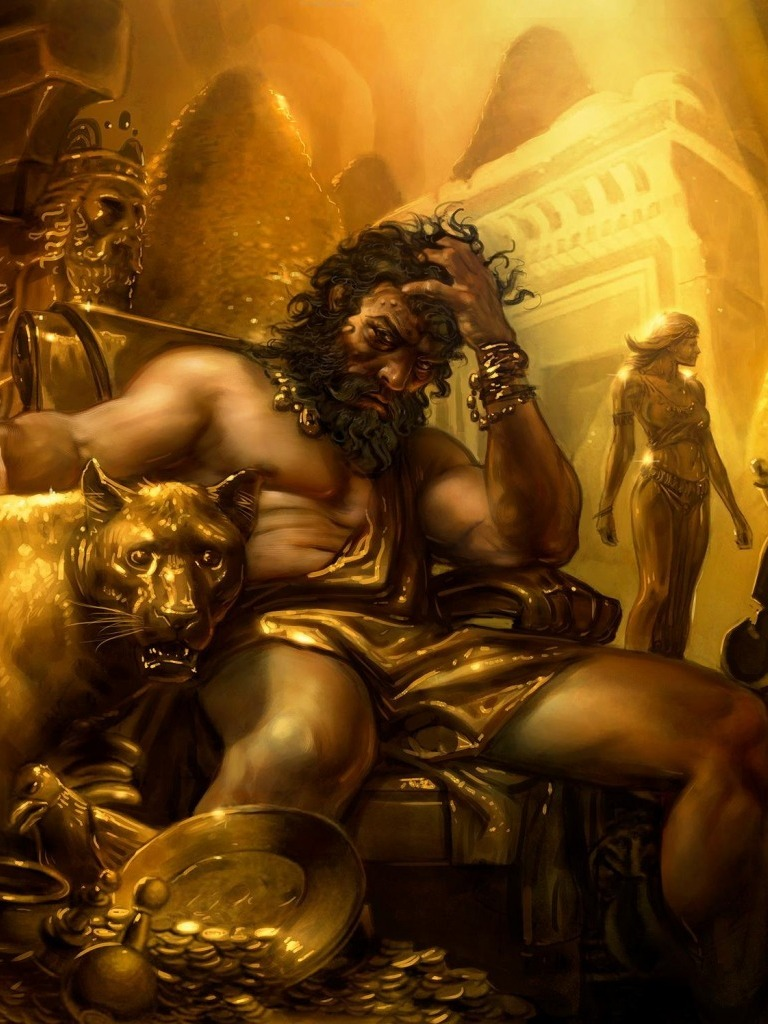
\includegraphics[width=3.5cm]{pathon.jpg}
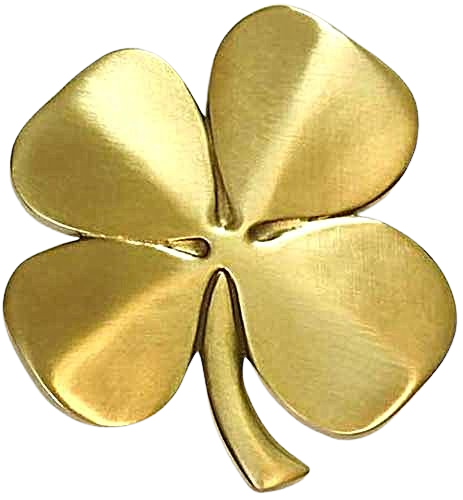
\includegraphics[width=3.5cm]{pathon_simbolo.png}
\subsection*{Sathona}
Sathona, dea degli inganni e delle menzogne è caotica malvagia. È protettrice degli impostori e ha il titolo di Regina Senza Volto. Veglia sulle menzogne e sui travestimenti. Viene venerata principalmente da ladri malvagi. È l'unica divinità malvagia che vive veramente nel Tatakai. I suoi domini sono Inganno, Male e Conoscenza. La sua arma preferita è il katar.\\
\\
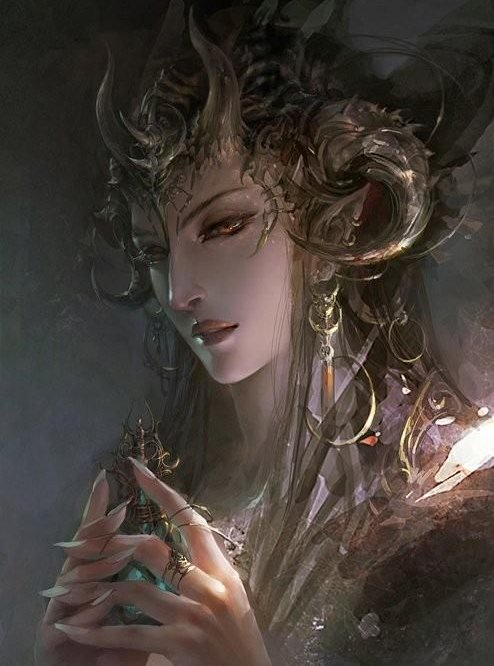
\includegraphics[width=3cm]{sathona.jpeg}
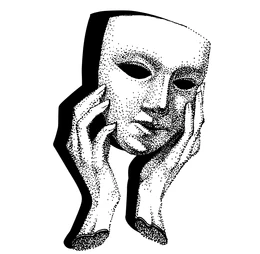
\includegraphics[width=3cm]{sathona_simbolo.png}
\subsection*{Tahia}
Tahia è la dea dell'odio, dell'invidia e dalla pazzia, di allineamento caotico malvagio. Invidiosa della bellezza della sorella Huaifu è la responsabile dell'odio e dell'invidia degli esseri mortali. Viene venerata dalle menti malvagie piene d'odio. A causa della sua pazzia è stata cacciata più volte dal Tatakai e dal Fukai (neanche quelli malvagi la vogliono); è stato infine raggiunto un accordo che la vuole confinata in uno spazio isolato del Fukai. I domini a lei associati sono Envy, Hatred, Madness e Male.
La sua arma prescelta è il pugnale.\\
\\
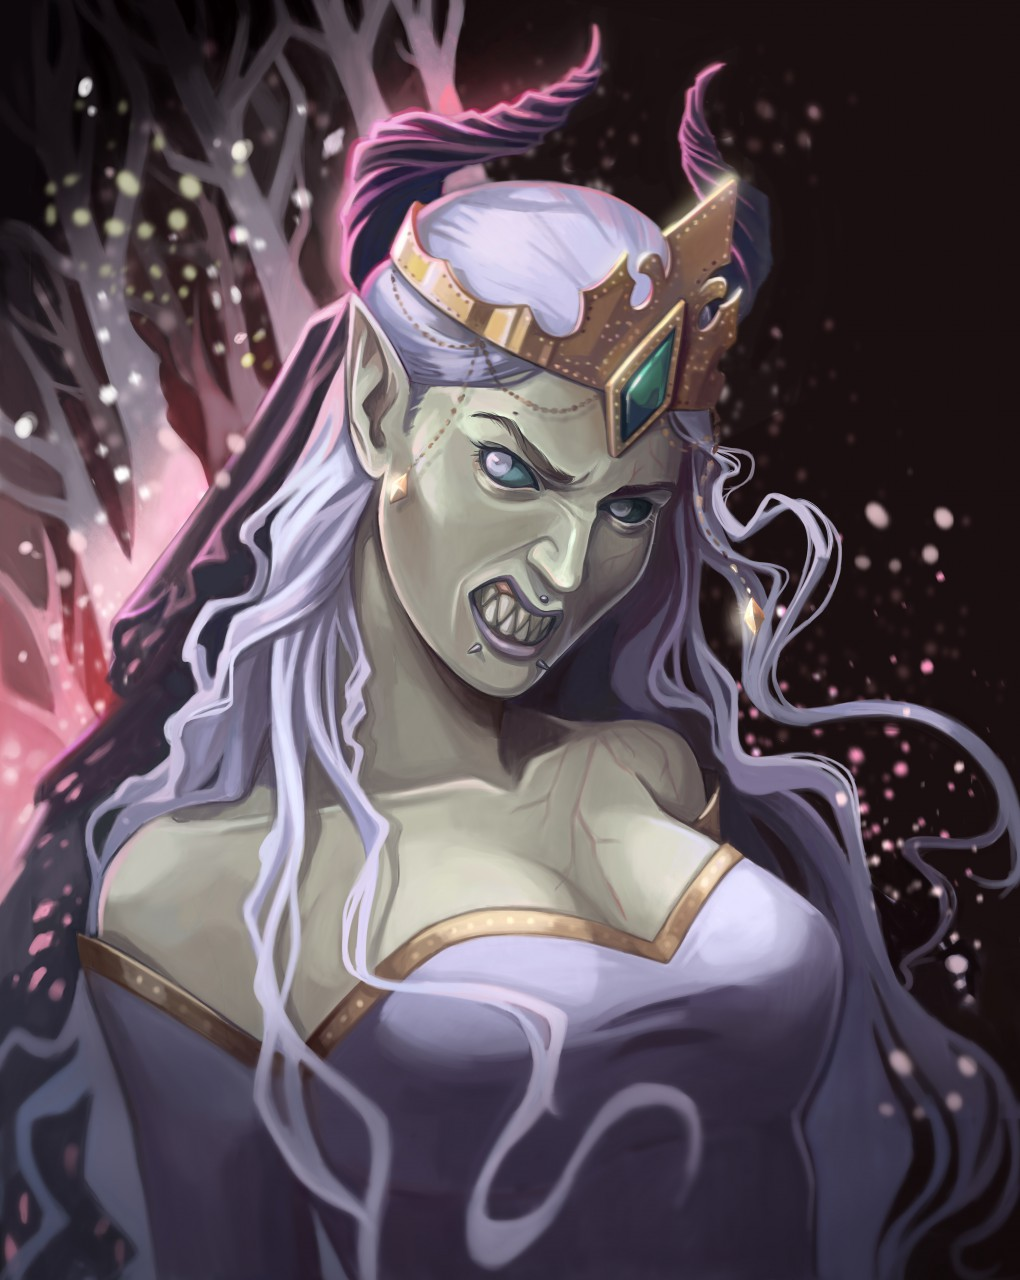
\includegraphics[width=3.5cm]{tahia.jpg}
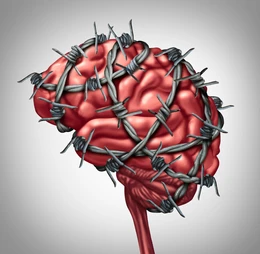
\includegraphics[width=3cm]{tahia_simbolo.png}
\subsection*{Talas}
Talas, dio del mare, del clima, dei venti e delle tempeste è di allineamento caotico neutrale. Viene raffigurato come un anziano con la barba del colore della schiuma del mare e coi capelli lunghi al vento. Spesso i marinai effettuano riti e sacrifici a Talas sperando di ottenere un clima favorevole durante i loro viaggi. Molti dei Cavalieri del Vento di Nausicaa sono suoi seguaci.
I suoi domini sono Ocean, Weather, Windstorm e Blackwater, mentre la sua arma prescelta è la rete.\\
\\
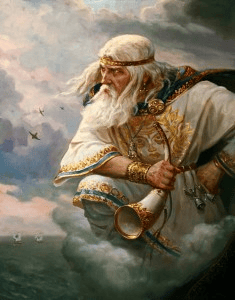
\includegraphics[width = 3.5cm]{talas.png}

\includegraphics[width = 3.6cm]{talas_simbolo.png}\\
\subsection*{Whest Falia}
Dio del commercio e della navigazione, Whest Falia, è neutrale. Conosciuto come Mercante di Stelle è il protettore dei commerci e dei marinai. Spesso i suoi fedeli sono anche bardi e più raramente ladri. Come Byrœ si trova molto spesso in giro per il Piano Materiale. I suoi domini sono Viaggio, Trade e Fortuna, la sua arma prescelta è il Naginata (Avventure Orientali).\\
\\
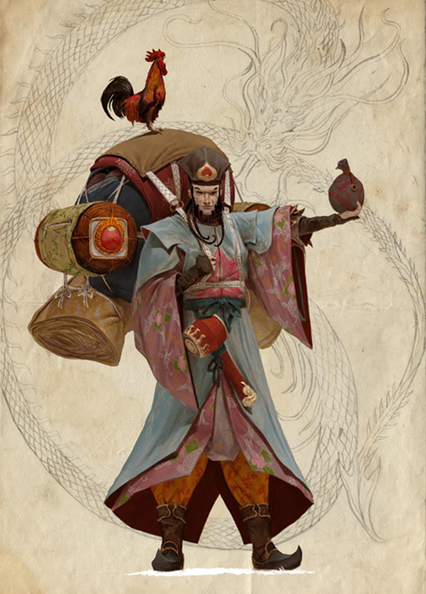
\includegraphics[width=3cm]{whestfalia.png}
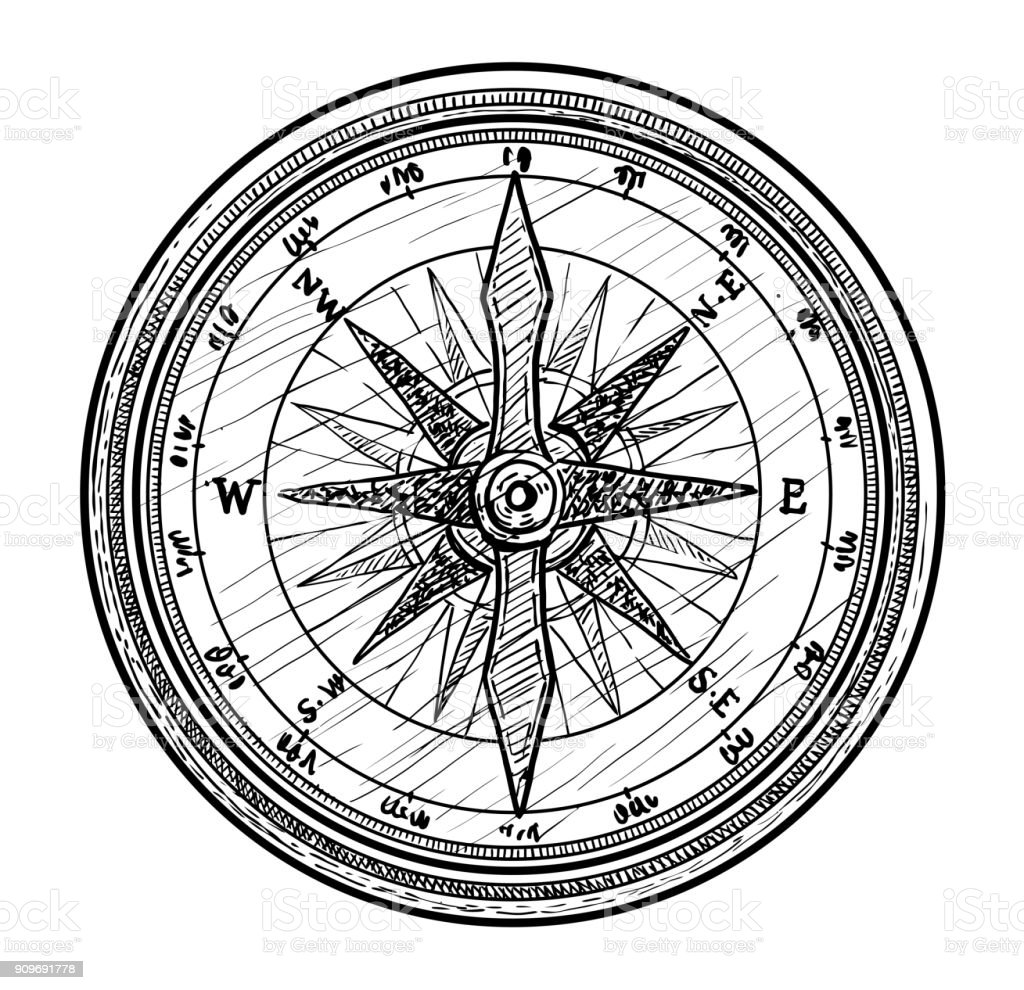
\includegraphics[width=3.5cm]{whestfalia_simbolo.jpeg}
\subsection*{Wrhat}
Wrhat è il dio della guerra e della distruzione, di allineamento caotico malvagio. È anche conosciuto come Il Funesto, Il Conquistatore e Il Sanguinario. Tra i suoi seguaci ci sono tutte le creature assetate di sangue oltre a barbari, paladini e guerrieri malvagi. A causa della sua malvagità è stato cacciato dal Tatakai, vive quindi nel Fukai. I domini a cui è associato sono Guerra, Caos, Male e Distruzione. La sua arma prediletta è la morning star.\\
\\
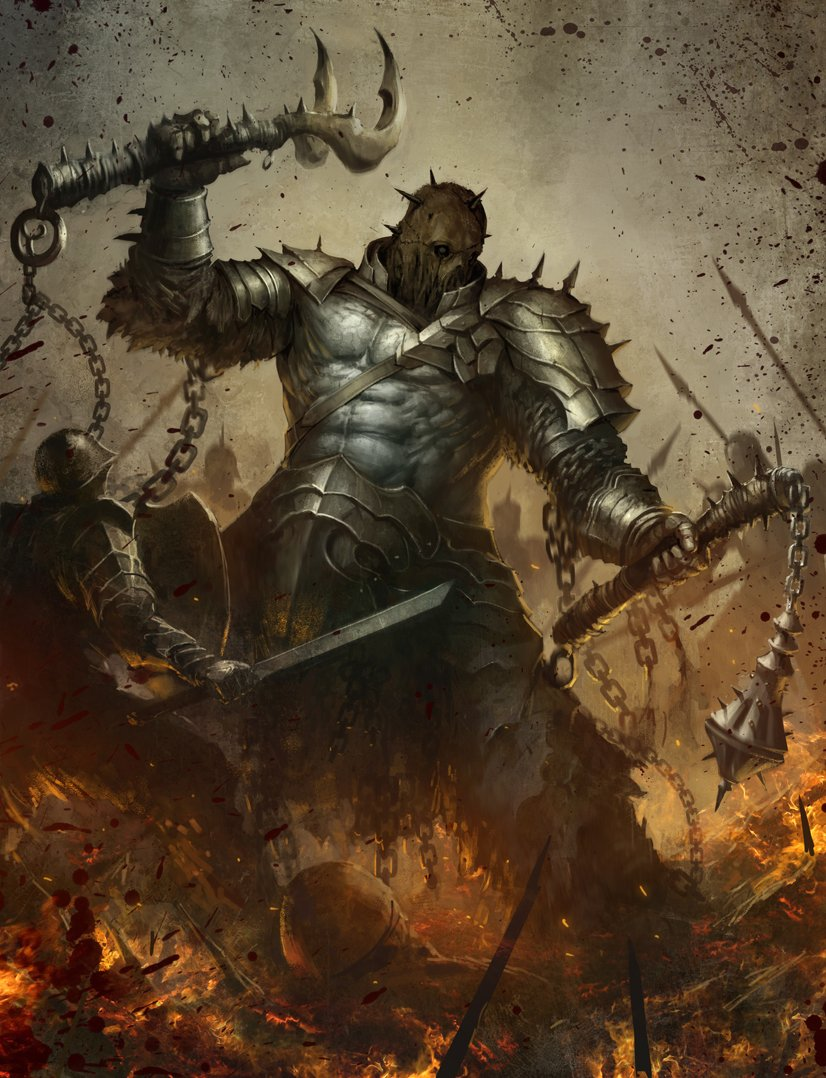
\includegraphics[width=3.5cm]{wrhat.jpeg}
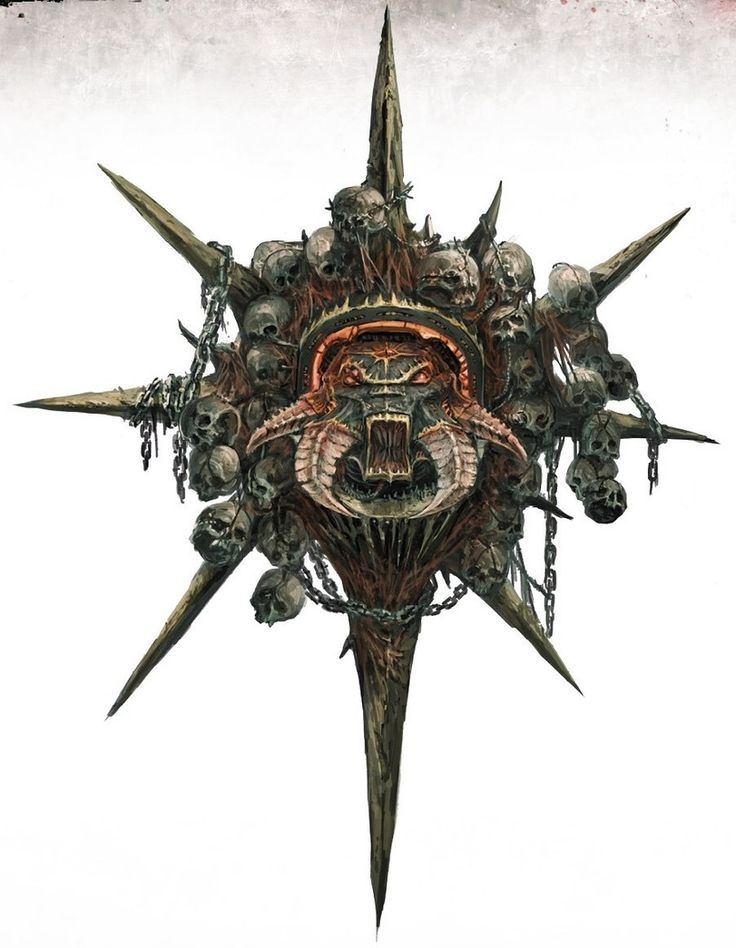
\includegraphics[width=3cm]{wrhat_simbolo.jpeg}
\subsection*{Yennifer}
Yannifer è la dea gnomesca della vita, delle piante e dell'erboristeria, di allineamento caotico buono. Ella è la creatrice dell'erboristeria e della farmacia, è rappresentata come una vecchia gnoma attrezzata per la cura e il trattamento delle piante. Viene venerata oltre che da gnomi anche da druidi e ranger di altre razze, o in generale da personaggi buoni. I domini a lei associati sono Life, Plant e Bene. La sua arma prescelta è il martello-picca gnomesco.\\
\\
\includegraphics[width=3.5cm]{yennifer.jpg}
\includegraphics[width=3cm]{yennifer_simbolo.jpeg}
\end{multicols}
\newpage
\begin{multicols}{2}
\section{Le Due Divinità Draghe}
\subsection*{Intense Yapping}
Cosa sono le divintà draconiche? Perché esistono? Da dove vengono? Cosa vogliono? Dove vanno? E soprattutto perché si meritano la loro personalissima \verb|\section{}|?
Ho letto le divinità del calva e sono rimasto colpito dal fascino di quelle draconiche al punto di freebootarle? \\
Senza nulla togliere al calva e alle sue divinità vorrei asserbarmi la carta freebooting per il futuro. Sappiate che le divinità draconiche sono due, e il motivo per cui hanno la loro personalissima sezione è che sono morte, e pure stronze. Per spiegare come mai erano stronze, segue un pippone sulle divinità draconiche e non.\\
Partiamo dagli Dei \enquote*{normali} (insomma quelli descritti nella sezione precedente); ognuno di loro ha degli obbiettivi, degli ideali che vuole diffondere nel mondo ed incaricano dei mortali a loro devoti, aka chierici, di seguire la loro volontà divina e diffonderla nel mondo dei mortali. I chierici in cambio ottengono poteri forniti direttamente dalla divinità che hanno lo scopo di aiutarli nella loro missione per servire il loro dio. Questo non sorprende nessuno perché è la base su cui è fondato il Chierico come classe. Questo meccanismo ha un effetto secondario, ovvero l'inevitabilmente stretto legame tra mondo divino e mondo dei mortali, e ciò rende le divinità\footnote{tecnicamente per come ho posto questo ragionamento si dovrebbe poter applicare tutti gli Dei, in qualsiasi ambientazione che ammetta l'esistenza dei chierici; ci limitiamo ad applicarlo esclusivamente alle nostre care divinità di Islena poiché sono le uniche rilevanti ai fini del discorso} \enquote*{umane} nei loro interessi e nei loro modi di agire e di interagire, sia con i mortali che tra di loro. Inoltre, come probabilmente vi ho già detto a voce ma lo ripeto qui per completezza, le divinità di questa ambientazione sono fortemente ispirate agli Dei Greci/Romani, sono per l'appunto molto \enquote*{umane}, commetto errori, hanno vizi e difetti e così via\footnote{Achtung! Questo non vuol dire che sono un branco di totali coglioni (in parte un pochino sì), rimangono comunque delle divinità e sono la massima espressione del concetto a loro legato.}. Per riassumere quindi le divinità sono imperfette nella loro essenza, sono strettamente legate al mondo dei mortali e ai mortali stessi tramite i chierici e soprattutto hanno interessi nel mondo dei mortali. \\
In cosa differivano le due divinità draconiche? Tutto, o quasi. Per iniziare non erano figlie dei Titani Elementali ma erano più loro simili, in quanto anche esse originarono dal caos della battaglia nel Tatakai, e rappresentavano una memoria di quello scontro tra Bene e Male. Inoltre erano completamente isolate dal mondo dei mortali e dalle altre divinità per un motivo principale, ovvero i loro interessi erano completamente autocontenuti, in quanto l'obbiettivo di uno era distruggere l'altro e viceversa. 
\newcolumn

Il loro conflitto stava mettendo fortemente a rischio l'intero cosmo, dunque gli altri Dei presero la decisione di ucciderli.
Segue una simpatica storiella eziologica, cantata da Byrœ, Il Dio Bardo in persona, sulle Divinità Draghe e sulla creazione dei draghi metallici e cromatici:

\begin{verse}
	\textit{In un'era primordiale, quando il cosmo vedeva i primi amori tra i Titani, nacquero due divinità draconiche: Ansur, Custode degli Eterei Cieli, e Engur, Signore delle Profondità Entropiche. Da subito, un'inesorabile forza le spinse in un fatal conflitto.\\
	Quando lo scontro tra i Draghi Primordiali minacciava di strappare il tessuto stesso del Mondo, le lamentele degli Dei risuonarono come una sinfonia funerea attraverso il Tatakai. \\
	Mentre alcuni sussurravano il loro dispiacere, le divinità guerriere, con spade ardenti e scudi inviolabili, avanzarono risolute verso l'epicentro del conflitto.\\
	Gli Dei affrontarono Ansur e Engur con la determinazione di chi combatte per la sopravvivenza del cosmo. \\Le loro lame fendevano l'aria, tracciando un'arcana coreografia contro le fiamme draconiche e le oscure tempeste.
	Il Cielo Stellato, teatro dell'epica battaglia, vide infine la funesta caduta delle divinità draconiche.\\
	Con occhi luminosi e voce che cullava l'universo, Byrœ cantò un'ode alla creazione; Dalle leggende degli scontri draconici plasmò nuove creature alate, che portavano il ricordo di quelle divinità ormai perdute.\\
	Così, il Mondo, salvato dalla rovina, vide la nascita dei draghi, guardiani e protagonisti delle epoche future. Il Padre dei Draghi aveva composto una nuova melodia nella partitura del cosmo, un'ode di vita e di speranza tra terre celesti e abissi profondi.}
\end{verse}

\newpage
\subsection*{Ansur}
Ansur, Custode degli Eterei Cieli. È rappresentato come un maestoso drago, col corpo composto da diversi metalli.\\
\\
\includegraphics[width=6cm]{gizzard.jpg}

\subsection*{Engur}
Engur, Signore delle Profondità Entropiche. È rappresentato come un minaccioso drago scuro, con sfumature dei colori dei draghi cromatici.\\
\\
\includegraphics[width=6cm]{engur.jpg}

\vspace*{1cm}

\end{multicols}
\begin{tiny}
	\textsl{Ma Signor DM, se queste divinità sono completamente inutili dato che sono morte, come mai ti sei preso la briga di inventartele, dargli dei nomi, e hai pure scritto una storiella per giustificare la loro inutilità? \footnote{Non rompete il cazzo.}}\\
\end{tiny}

\vspace{1cm}
\begin{table}[h]
\centering
{\sffamily
\begin{tabular}{||c|c||}
\hline
\bf	Razza & \bf Divinità\\
\hline
Umano & Per classe e allineamento\\
\hline
Nano & As Vahal o per classe e allineamento\\
\hline
Elfo & \quad \quad \quad \quad \quad \quad Bhar B'Hero, Hnana o per classe e allineamento \quad \quad \quad \quad \quad \quad\\
\hline
Gnomo & Yennifer, Hnana o per classe e allineamento\\
\hline
Mezzelfo & Althes, Bhar B'Hero, Hnana o per classe e allineamento\\
\hline 
Mezzorco & Fjorsh o per classe e allineamento\\
\hline
Halfling & Djenl, Hnana o per classe e allineamento\\
\hline
Azuril & Talas, Whest Falia o per classe e allineamento\\
\hline
\end{tabular}
}
\caption{Divinità per razza}
\end{table}

\begin{table}[h]
\centering
{\sffamily
\begin{tabular}{||c|c||}
\hline
\bf Classe & \bf Divinità(Allineamento)\\
\hline
Barbaro & Talas(CN), Wrhat(CM)\\
\hline
Bardo & \quad Byrœ(CN), Huaifu(CB), Bhar B'Hero(N), Pathon(N), Whest Falia(N), \quad \\
\hline
Chierico & Qualsiasi\\
\hline
Druido & Hnana(NB), Yennifer(CB)\\
\hline
Guerriero & Cha Ah'ad(LN), Wrhat(CM), Kygeus(LB), Cloit(LN), Claef(NB) e Cleos(N), Immaru(LM)\\
\hline
Ladro & Sathona(CM), Pathon(N), Lialgha(NM)\\
\hline
Mago & Bhar B'Hero(N), Moohona(N), Lialgha(NM)\\
\hline
Monaco & Kygeus(LB), Immaru(LM), Cha Ah'ad(LN), Fjorsh(NB)\\
\hline
Paladino & Qualsiasi\\
\hline
Ranger & Hnana(NB), Althes(N)\\
\hline
Stregone & Moohona(N), Lialgha(NM)\\
\hline
\end{tabular}
}
\caption{Divinità per classe}
\end{table}

\chapter{La Magia Arcana}

\begin{multicols}{2}

\section{Origine} 
La magia arcana è stata creata da Moohona, come concetto e come disciplina. L'origine di quest'arte è narrata da Byrœ nella seguente leggenda:

\begin{verse}
	
\textit{In un'era antica, quando il creato era un canto appena intonato e gli Dei tracciavano la loro dimora nel Tatakai, Moohna, la sublime Maga Celeste, sedeva pensosa sul margine del firmamento.\\ Ella scrutava il Mare di Stelle, quell’incommensurabile abisso scintillante che sussurrava segreti arcani al di là del velo del comprensibile.
Fu allora che il suo sguardo divino si posò su una luce inusuale, più viva e tremula di tutte le altre.\\ Una stella che sembrava pulsare come il cuore stesso dell'universo, una scintilla di potere pura e separata, un'energia che nulla nel mondo conosciuto avrebbe potuto eguagliare.\\ In quel bagliore, la Dea percepì una verità primordiale, un concetto che non esisteva ma che doveva nascere nel cuore stesso della sua mente divina: la magia arcana, una forza distinta che nulla di ciò che esisteva fino a quel momento poteva governare.\\ Spinta dal desiderio di donare al mondo ciò che aveva visto, Moohna tese la mano, e con gesto solenne afferrò quella luce. Il Mare di Stelle, come sospeso, trattenne il respiro.\\ Quando riaprì il palmo, la stella non era più luce, ma una pietra di bellezza straordinaria, lucente come il cielo stesso, cangiante nei colori di aurore e tramonti. Era la prima scintipietra, un frammento tangibile di quella potenza che ella aveva concepito, ma che era al di fuori della realtà ordinaria.\\
Eppure, la Dea capì che la sua creazione non doveva restare una prerogativa divina. La pietra, sebbene fatta di potenza incommensurabile, era destinata ad altri, era il tramite per attingere a quella forza separata che ella aveva creato.}
\end{verse}
\newcolumn
\begin{verse}
\textit{Ma ella sapeva che i mortali, con le loro menti limitate, non sarebbero stati in grado di cogliere la natura originaria di quel potere. Loro non avrebbero potuto vedere, come lei, il concetto puro nel cuore della stella. \\
Ella così scese tra i mortali, li fece radunare sotto il cielo stellato, e, con voce che risuonava come un canto eterno, disse loro:\\
\enquote*{O figli della terra, il cielo che vi sovrasta è il riflesso di un cosmo ben più grande, un’immagine distorta e lontana del Mare di Stelle che io sola posso contemplare. Non cercate di vedere ciò che è nascosto ai vostri occhi mortali, né tentate di afferrare ciò che non è destinato alla vostra comprensione. Ma sappiate questo: in ogni stella che brilla nel cielo si cela una scintilla del mio potere, una scintilla che può illuminare il cammino di chi sa vedere oltre l’apparenza. Studiate il cielo sopra di voi, guardate nei suoi schemi e nei suoi disegni, cercate la scintilla che parla al vostro spirito e lasciate che vi guidi. Vi guiderà nel creare la scintipietra, essa sarà il vostro legame con il potere arcano, il vostro ponte tra ciò che è e ciò che può essere.}\\
Da quel giorno, la magia si diffuse nel mondo, non come dono o potere concesso, ma come una disciplina, un’arte che richiede studio e introspezione. Ogni frammento di scintipietra è un testamento dell’intimo legame tra il mortale e l’infinito, un ponte tra la terra e il cielo, tra ciò che si può conoscere e ciò che si deve cercare in eterno.\\ Si narra che, ancora oggi, ogni volta che un mortale forgia una scintipietra, un tremolio attraversi le stelle, un’eco del momento in cui Moohna afferrò la prima luce.}
\end{verse}

\includegraphics[width=6cm]{monascintipietra.jpeg}

\section{Scintipietra}
Mentre gli incantatori divini ottengono i loro poteri magici dal loro legame con entità di natura divina, gli incantatori arcani di Islena traggono la loro magia dalla scintipietra. Ogni incantatore arcano deve avere un frammento di scintipietra sulla sua persona se vuole lanciare un incantesimo. Anche nelle bacchette, o molti altri oggetti magici che replicano incantesimi, ci sono frammenti o polvere di scintipietra. Ovviamente non tutti gli incantatori arcani interagiscono con la scintipietra allo stesso modo:

\subsection*{Maghi}
I maghi sono stati i primi a brandire la magia arcana, ogni mago segue l'insegnamento di Moohna e crea la propria scintipietra dallo studio metodico del cielo stellato. Dopo la creazione della propria scintipietra, lo studio del mago continua per l'apprendimento di nuovi e più potenti incantesimi. Spesso i maghi incastonano la loro scintipietra nella copertina del loro libro degli incantesimi.
	
\subsection*{Stregoni}
Gli stregoni, a differenza dei maghi, di solito non si interessano allo studio del cielo e molto raramente creano la propria scintipietra. Spesso il cammino dello stregone inizia dopo aver trovato per caso o aver acquistato un frammento di scintipietra, dopo di che, senza troppo bisogno di studi e riflessioni lo stregone riesce a entrarci in comunione, traendone così i suoi primi poteri magici. In pratica lo stregone medio vede i maghi che lanciano incantesimi apparentemente solo tramite questa pietra, pensa di poter fare lo stesso e poiché ci crede abbastanza, lo fa, senza bisogno di intenso studio. Più lo stregone acquista confidenza con l'utilizzo della scintipietra e più diventa potente apprendendo incantesimi nuovi. Gli stregoni portano la loro scintipietra in vari modi, chi sulla punta di un bastone, chi al collo con un amuleto ecc. 


\subsection*{Bardi}
Ci sono varie scuole di pensiero tra i bardi. C'è chi crea la propria scintipietra dall'osservazione del cielo, ma in questo caso, a differenza del mago, l'occhio del bardo ricerca nelle costellazioni immagini artistiche, che raccontino storie o schemi musicali ecc. Altri bardi preferiscono acquistare la loro scintipietra e ricercano in essa il legame con la loro arte. Solitamente al bardo piace narrare la storia di come ha ottenuto la sua scintipietra e le sue capacità magiche. Un bardo che si esercita nelle sue abilità artistiche rafforza il legame con la scintipietra e migliora come incantatore.
Come gli stregoni i bardi custodiscono la loro scintipietra in una multitudine di modalità.  

\subsection*{Altri incantatori arcani}
In generale si possono considerare Maghi, Stregoni e Bardi come tre macro-categorie nelle quali ricadono bene o male tutti gli altri incantatori arcani (ad esempio un Wu-Jen è praticamente un mago). Warlock e simili non hanno bisogno della scintipietra per le loro invocazioni.

\section{Legame tra magia e scintipietra: Le implicazioni}
L'implicazione principale è che la scintipietra diventa una merce di scambio, esistono compagnie di maghi che creano e vendono scintipietra, e magari nel mercato nero si trova a prezzi più competitivi. In generale un frammento di scintipietra, delle dimensioni adatte al lancio di incantesimi, di media qualità, costa poche decine di monete d'oro (30-50mo). Frammenti più piccoli o polvere di scintipietra usate nella creazione di bacchette e altri oggetti magici si trovano a poche monete d'oro (1-3mo).

Un'implicazione minore è che adesso anche stregoni e bardi sono esposti allo stesso rischio che i maghi corrono, ovvero perdere il proprio libro degli incantesimi o frammento di scintipietra.


\end{multicols}

\part{Islena}

\chapter{Storia}
\begin{multicols}{2}	
	In questa sezione è raccontata in breve la storia del continente. La storia dei singoli stati verrà esplorata nella sezione Regni quando necessario. 
\section*{Le Dieci Famiglie}
Più di 2000 anni fa Islena era governata dalle dieci famiglie colonizzatrici, cinque si dividevano i territori dell'Est e le altre cinque si spartivano l'Ovest. Le Famiglie era bene o male in grado di mantenere la pace nel continente e non si hanno notizie di grandi conflitti tra di esse. Come ogni famiglia amministrasse il proprio territorio è ignoto e gran parte delle informazioni su di esse sono andate perdute. 
\section*{Il Popolo del Mare}
La pace venne bruscamente interrotta da un’invasione esterna; un misterioso popolo guerriero passato alla storia come Popolo del Mare raggiunse le coste di Islena e mise al sacco i territori dell’Est. Gli eserciti delle famiglie non potevano niente di fronte all’inarrestabile forza del Popolo del Mare. Nel giro di pochi mesi l’intera metà orientale di Islena venne occupata dal Popolo del Mare.\\
Improvvisamente e misteriosamente, una volta conquistato l’Est, il Popolo del Mare si ritirò e abbandonò Islena senza lasciare nessuna traccia, per mai più fare ritorno. \\
Forse neanche gli Dei conoscono le intenzioni del Popolo del Mare e i motivi della ritirata, gli storici mortali moderni non hanno nessuna informazione su di essi e ancora non comprendono come mai venne interrotta improvvisamente l’avanzata. 
\section*{La Guerra dei Quoti}
Dopo la ritirata del Popolo del Mare le famiglie dell’Ovest spinte dall’ambizione e dalla superbia si allearono e organizzarono gli eserciti con l’intento di conquistare i territori orientali approfittando della rovina delle famiglie dell’Est. Nel frattempo ad oriente dalle ceneri dell’invasione nacquero i Quoti: un ordine di potenti guerrieri che si pose l’obbiettivo di difendere il continente dalla tirannia delle famiglie dell’Ovest corrotte dalla sete di potere e di riportare la pace a Islena. La loro origine è tutt’oggi avvolta nella leggenda.Conflitti di interessi interni alle famiglie dell’Ovest furono motivo dello scoordinamento dei primi attacchi, che vennero dunque respinti dall’incredibile potere dei Quoti. Con queste premesse ebbe inizio la leggendaria Guerra dei Quoti che andrà avanti per poco meno di un secolo e vedrà la sua fine con la vittoria dei Quoti.\\
La fine della Guerra dei Quoti corrisponde con l’anno 0.
\section*{I Secoli Ubertosi e il Tradimento Ouster}
Dopo la guerra i Quoti avevano ottenuto il controllo sull’intero continente, grazie al loro sovrumano potere riuscirono dunque a governare Islena per svariati secoli, tramite un Consiglio ristretto centrale formato dai 30 Grammaestri Quoti. Questi valorosi guerrieri erano però mortali e quindi avevano spesso apprendisti che addestravano per poter passare il testimone e tramandare il grande potere e la grande responsabilità dei Quoti. A questo periodo risalgono le rovine che si trovano in giro per Islena al giorno d’oggi, simbolo di una grande civiltà dimenticata. Nel 746esimo il Grammaestro Ouster, inavidito e corrotto dalla ricerca di potere, con l’aiuto di alcuni suoi allievi commise 7 omicidi ai danni di altri Grammaestri, con l’intento di assumere il controllo di Islena e fondare un impero continentale. Sorse il caos totale nel Consiglio e nell’intero continente. I Grammaestri persero la fiducia gli uni negli altri e nelle province più periferiche di Islena, data l’instabilità del governo centrale, sorsero i primi stati indipendenti.
\section*{Dall'Ultima Battaglia ai giorni nostri}
I piani del Grammaestro Ouster vennero infine svelati, portando i Grammaestri a tentare di arrestarlo. Nel 751esimo anno scoppiò una devastante battaglia conosciuta come l'Ultima Battaglia. Ouster emerse vittorioso insieme ai suoi sostenitori, ma il sogno di un impero continentale si infranse a causa dei conflitti interni tra i traditori.
Con la caduta del Consiglio dei Quoti, oltre al sorgere dei primi stati indipendenti nacque il breve Impero di Ouster, che si sgretolò rapidamente dopo la sua sconfitta per mano dei suoi due allievi più potenti, Unduli e Hooke. Dopo la morte di Ouster gran parte del continente fu contesa tra il Vecchio Mos, sotto il controllo di Unduli, e l'Impero di Hooke.
La guerra tra Unduli e Hooke fu breve ma intensa, culminando nella loro reciproca distruzione. I territori di Unduli rimasero uniti nel Nuovo Mos, sotto il potere sempre minore degli ultimi suoi sostenitori. L'Impero di Hooke si frammentò negli antenati dei vari stati orientali odierni.
Hooke e Unduli furono gli ultimi in grado di maneggiare il mistico potere dei Quoti.
Nonostante la tragica fine dei Quoti sia relativamente recente, essi vennero presto dimenticati. I loro edifici e infrastrutture furono abbandonati, e la loro storia divenne leggenda. Nell'ideale comune, l'epoca dei Quoti sembra appartenere a un millennio più antico di quanto sia realmente.


\end{multicols}

\chapter{Carattere del Continente}

\begin{multicols}{2}
In questa sezione voglio darvi una breve descrizione del carattere generale del continente e come appare al giorno d’oggi prima di inoltrarci nei dettagli dei vari stati. Non so bene come mettere per scritto l’idea che ho di Islena, quindi se avete domande chiedete pure, molto probabilmente alcune cose ve le dirò anche a voce anche mentre si gioca.

\section{Elementi Generali}
\subsection*{Caratteri Steam-Punk}
Alcune regioni di Islena (in seguito verrà specificato quali in particolare) stanno attraversando un periodo di progresso magico-scientifico che sta portando verso uno sviluppo tecnologico. Non è una roba tipo Rivoluzione Industriale, ma seppur il carattere principale di Islena rimane medievaleggiante (stile Grayhawk insomma) in secondo piano ci saranno elementi steam-punk.\\
Quando (o se) visiterete queste regioni ve lo dirò e dovrete spesso fare lo sforzo di immaginarvi questi tratti steam-punk intrecciati con la realtà medievale a cui siamo abituati senza che io stia troppo a descriverli (per non rendere la cosa pallosa).

\subsection*{Segni di un'antica civiltà}
Un altro importante aspetto sono le rovine risalenti all’epoca del Quoti, presenti in tutta Islena saranno molto comuni nelle vostre avventure. Come ho già accennato nella sezione Storia, il sentimento comune è quello che i Quoti abbiano governato Islena più di mille anni fa (mentre in realtà sono passati circa 400 anni), questo è sia causa che conseguenza del fatto che questi edifici siano lasciati in rovina. Ovviamente quando dei luoghi saranno rilevanti ai fini del gioco ve li indicherò, ma come per gli elementi steam-punk, spesso dovrete fare lo sforzo di immaginarvi per conto vostro la loro presenza: ad esempio se state viaggiando nelle famose \enquote*{terre selvagge} non posso dirvi ogni due minuti che vedete delle rovine, però dovete immaginarvele e far in modo che siano una presenza abbastanza costante nell’immaginazione delle vostre avventure (non preoccupatevi comunque vi aiuterò spesso, soprattutto nelle città che visitate magari alcuni edifici sono sorti sopra queste rovine e in quei momenti ci penserò io a descrivervi l’ambiente). Ecco qualche immagine che possa farvi capire di stile di rovine si tratta e come queste spesso siano inglobate nelle città e nella vita quotidiana:\\

\includegraphics[width=7cm]{ruins.png}\\

\includegraphics[width=7cm]{insideruins.jpg}\\

\includegraphics[width=7cm]{ruinsincity.jpg}\\

\includegraphics[width=7cm]{ruinsinwall.png}\\
\end{multicols}

\newpage
\begin{multicols}{2}
\section{Le Culture} 
Con \enquote*{culture} intendo stile generale di un luogo; architettura, cibo, vestiti ecc. L’appartenenza a una razza non implica necessariamente l’appartenenza a una cultura specifica; sia le razze che le culture sono dipendenti dal territorio ma la loro diffusione non è sovrapposta perfettamente (anche perché ci sono più razze che culture). In questa sezione vi racconto quelle che sono le culture principali; esistono delle ramificazioni di queste che possono differire nei dettagli minori (piatti tipici, tradizioni popolari e cose così).\\
Come per le divinità se avete richieste particolari si possono tranquillamente creare culture nuove a vostro piacimento prima che si inizi a giocare (probabilmente da qui a là anche io aggiungerò qualcosa), se non avete richieste particolari siete comunque liberi di divertirvi a pensare a qualche dettaglio del luogo da cui provenite, nel quale potrebbe esserci una delle ramificazioni di cui parlavo. \\
\\
Le culture principali del continente (a cui	ho dato nomi solamente per distinguerli tra di noi, in realtà non usati tra la gente di Islena che non fa proprio queste distinzioni) sono:\\

\begin{itemize}
	\item I Nord: Come dice il nome la cultura Nord è diffusa al nord di Islena, in particolare al nord-est, nelle regioni più fredde. Il carattere di questa cultura è vichinghesco e skyrimmiano, e fa riferimento alla cultura Norrena.\\
	\\
	\includegraphics[width=6cm]{nord.jpg}
	\\
	\\
	
	\item Gli Slenici: La cultura Slenica è quella di gran lunga più diffusa. Rappresenta la classica cultura medievalesca europea, nulla di particolare.\\
	\\
	\includegraphics[width=6cm]{islenici.jpg}
	\\
	
	\item Gli Injines: È la cultura meno diffusa, presente solo in una regione del nord, ma sicuramente la più particolare: È infatti un misto di cultura indiana e giapponese/asiatica con elementi random spagnoleggianti.\\
	\\
	\includegraphics[width=6cm]{injines.jpg}
	\\
	
	\item Gli Arabas: Cultura diffusa in una regione desertica, caratterizzata da elementi arabeggianti e dotraki.\\
	\\
	\includegraphics[width=6cm]{arabas.jpg}
	\\
	
	\item Gli Egisci: Anche loro abitano una regione desertica e sono ispirati agli antichi egizi.\\
	\\
	\includegraphics[width=6cm]{egisci.jpg}
	
	\item I Felezi: Cultura diffusa in un territorio giungloso (tipo Sud America), ispirata principalmente all'antica Mesopotamia, con elementi Maya e indigeni/tribali. \\
	\\
	\includegraphics[width=6cm]{felezi.jpg} 
	\\

	\item I Gerici: Cultura ampiamente diffusa sulle coste orientali. È la cultura caratterizzata dagli elementi steam-punk, di cui si è già parlato, su una base simile all'antica Grecia ma un po' più sobria. Ripeto che la roba steam-punk è in secondo piano e è molto più legata alla magia che alla scienza.\\
	\\
	\includegraphics[width=6cm]{gerici.jpg}	
	\\

	\item I Silvanesi: La cultura silvanese è diffusa in aree boschive e fortestal del sud-est e sud-ovest. È ispirata alla classica architettura elfica tipo Lord of the Rings, ma non è esclusiva agli elfi, anche se molto presenti in queste zone.\\
	\\
	\includegraphics[width=6cm]{silvanese.png}
\end{itemize}
\vspace{4cm}
\subsection*{Divinità e Culture}
Ci tengo a specificare che le divinità sono le stesse in tutto il continente, ciò che può variare sono le rappresentazioni di esse da parte di ciascuna cultura. \\
Ad esempio una rappresentazione egiscia di Moohona potrebbe essere qualcosa del genere:\\
%\footnote{Dopo una lunga e intensa battaglia devo dichiarare la mia sconfitta e arrendermi al fatto che questa immagine sia destinata, per nessun apparente motivo, a stare a destra del testo}
\\

\includegraphics[width=7cm]{moonaegisci.jpg}
\end{multicols}
\vspace{1cm}
\subsection{Mappa delle Culture di Islena}
\begin{figure}[h!]
	\centering
	\includegraphics[width=18cm]{islenacultures.png}
	\caption{Mappa delle Culture. In viola i Nord, in celeste gli Slenici, in rosa scuro i Silvanesi, in arancione gli Arabas, in rosso gli injines, in blu gli Egisci, in verde i Felezi, in giallo i Gerici}
\end{figure}
\newpage
\begin{multicols}{2}
\section{Il Calendario}
		Il calendario in uso è molto semplice e sobrio. Un anno è composto da 330 giorni suddivisi in 11 mesi da 30 giorni ciascuno. Ogni mese è composto da 5 settimane da 6 giorni (ok non sono settimane si dovrebbero chiamare seimane ma fottesega). Le festività sono 4 e successivamente verranno descritte molto brevemente brevemente.
	\subsection*{Giorni Scarlatti}
		La festa dei Giorni Scarlatti si svolge nei primi 9 giorni del mese di Fresco ed è rivolta all'adorazione della Dea Huaifu, viene celebrato l'ammore e solitamente i matrimoni avvengono in questo periodo. Le città più grandi e ricche espongono per le strade decorazioni di colore rosso. Inoltre i cittadini girano mascherati (con maschere tipo carnevale di Venezia) e organizzano balli e giochi nelle città.
	\subsection*{Solstizio degli Eroi}
		Il Solstizio degli Eroi si tiene nei primi 9 giorni del mese di Foato, e celebra l'inizio dell'estate e le imprese degli eroi. Nelle città vengono organizzati tornei con diversi premi in palio, ovviamente più ricca la città più ricco il premio. Nelle città più importanti si tengono i tornei più prestigiosi ai quali partecipano gli eroi più valorosi.
	\subsection*{Festival delle Anime Perdute}
		Il Festival delle Anime Perdute si svolge durante i primi 9 giorni del mese di Vendemmiativo ed è rivolta al ricordo dei morti. È una festa a sfondo molto religioso, per le città si organizzano processioni e riti per scacciare la morte.
	\subsection*{Aurora}
		L'Aurora si tiene gli ultimi 9 giorni dell'anno e celebra la fine dell'anno e augura un buon inizio per il successivo. Le città più ricche e grandi espongono decorazioni di colore oro e argento. La tradizione prevede lo scambio di dolci tra i familiari e gli amici.
\end{multicols}
	\vspace{1cm}
	\begin{table}[h]
		\centering
		\begin{tabular}{||ccc||}
			\bf Giorno & & \bf Attività\\
			Kygedì & & Lavoro\\
			Hnanedì & & Lavoro\\
			Huaifedì & & Lavoro\\
			Moohonedì & & Lavoro\\
			Pathedì & & Riposo\\
			Coepiedì & & Adorazione\\
		\end{tabular}
		\caption{La seimana}
	\end{table}
\vspace{1cm}
	\begin{table}[h]
		\centering
		\begin{tabular}{||ccc||}
			\bf Mese/Festività  & & \bf Stagione \\
			Levante & & Inverno\\
			Fresco/Giorni Scarlatti & & Inverno/Primavera\\
			Risveglio & & Primavera\\
			Floraio & & Primavera\\
			Foato/Solstizio degli eroi & & Estate\\
			Coepio & & Estate\\
			Lumido & & Estate\\
			Brumaio & & Autunno\\
			Vendemmiativo/Festival dei Perduti & & Autunno\\
			Cadente & & Autunno/Inverno\\ 
			Diacciaio/Aurora & & Inverno\\
		\end{tabular}
		\caption{Gli 11 mesi e le 4 festività}
	\end{table}
	\newpage


\chapter{Reami di Islena}
\begin{multicols}{2}
	
\section{Introduzione ai Reami}
In questo capitolo verranno descritti gli stati di Islena per come sono al giorno d'oggi ovvero nell'anno 1183esimo. Cercherò dove possibile di fornire alcune notizie sulla storia dei singoli stati, se interessante. Le città elencate sono solo alcune, altre potrebbero essere aggiunte nel corso del tempo.
\section{Descrizione dei Reami}

\subsection*{Ajedij}
\begin{itemize}
	\item \textbf{Nome appropriato:} Sultanato di Ajediyabu
	\item \textbf{Sovrano: }Altissimo Uordsiti il Solenne, Umano NM
	\item \textbf{Governo: }Monarchia assoluta del Sultano a successione ereditaria di stampo feudale. Il Sultano è assistito da un consiglio di visir e consiglieri, che lo aiutano nelle decisioni politiche e amministrative.
	\item \textbf{Città: }Cheuta(GC), Labet(GP)
	\item \textbf{Risorse:}  oro, gioielli, tessuti, datteri, vetro, grano.
	\item \textbf{Popolazione e Cultura:} Egiscia, Umani 69\%, Gnomi 17\%, Halfling 12\%, Altro 2\% 
	\item \textbf{Legge: }LM
	\item \textbf{Situazione diplomatica: }Impegnato nell'Alleanza Triangolare insieme al Ducato di Al Mokha e All'Emirato Kstatungterkiano, basata su accordi commerciali e di non belligeranza. Accordi commerciali con Neverland.
\end{itemize}
Il Sultanato di Ajedij si estende attraverso vaste distese desertiche, la cultura del sultanato è profondamente influenzata dalle antiche tradizioni nomadi, che si mescolano con le più sofisticate pratiche urbane delle città principali. La società ajedijiana è stratificata, con una netta distinzione tra nobili, mercanti, artigiani e contadini. Le oasi permettono un'agricoltura limitata ma molto produttiva, con colture come datteri, grano e spezie. \`{E} presente un esercito decentemente addestrato per difendere le poche terre fertili. Il Sultanato è ricco di leggende e miti che parlano di creature misteriose che abitano il deserto.

\subsection*{Al Mohlka}
\begin{itemize}
	\item \textbf{Nome appropriato:} Ducato Divino di Al Mohlka
	\item \textbf{Sovrano: }Lacio Spacho Il Tiranno Divino, Umano NM
	\item \textbf{Governo: }Potere centralizzato nella figura del Duca Divino, che unisce potere temporale e spirituale. Il consiglio degli dei Sacerdoti lo assiste nella gestione del ducato.
	\item \textbf{Città: }Tasab(GC), Duwairah(GP)
	\item \textbf{Risorse:}  bestiame, spezie, incenso, tappeti, tessuti.
	\item \textbf{Popolazione e Cultura:} Arabas, Umani 59\%, Nani 17\%, Halfling 12\%, Mezzorchi 10\%, Altro 2\% 
	\item \textbf{Legge:} LN
	\item \textbf{Situazione diplomatica: }Impegnato nell'Alleanza Triangolare insieme al Sultanato di Ajedij e All'Emirato Kstatungterkiano, basata su accordi commerciali e di non belligeranza. Alleati: Rocciafertia.
\end{itemize}
Al Molkha nacque dalle unioni di diverse tribù nomadi del deserto, riunite sotto un unico comando. Le leggende narrano che il primo Duca Divino ricevette una visione dalla divinità protettrice del deserto, che lo incaricò di unificare il popolo e guidarlo verso la prosperità.  La società di Al Molkha è profondamente religiosa e organizzata secondo rigidi valori tradizionali. Per secoli, i Duchi Divini hanno mantenuto stabilità e prosperità attraverso un governo giusto e rispettoso delle necessità della popolazione, equilibrando gli interessi delle tribù, distribuendo equamente le risorse, guidando così lo stato a una notevole crescita economica.
Il più recente Duca tuttavia, ha attuato una politica diversa. Le sue decisioni arbitrarie e la negligenza verso gli interessi delle tribù hanno alimentato divisioni interne e malcontento. La sua gestione imprudente ha portato al declino economico e sociale, mettendo a rischio il futuro del ducato. 
L'economia di Al Molkha è diversificata nonostante l'ambiente ostile. Le oasi permettono la coltivazione di datteri, grano e ortaggi, oltre all'allevamento di cammelli e pecore. Il commercio è facilitato dalle rotte carovaniere che attraversano il ducato.

\subsection*{Aruba}
\begin{itemize}
	\item \textbf{Nome appropriato:} Repubblica Ribelle di Zion e delle Terre di Aruba
	\item \textbf{Sovrano:} Grande Maestro Sifo Dyas Camerlengo del Concistoro della Ribellione, Generale della Milizia delle Ali Bianche, Maestro dell’Ordine dei Combattenti della Spada Alata, Soprintendente di Zion, Azuril, LB
	\item \textbf{Governo:} Stratocrazia retta dal Concistoro della Ribellione con a capo il Camerlengo, carica eletta dal Concistoro tra i membri del Concistoro Ristretto,; vi è anche il Tribunato del Popolo di Aruba, organo legislativo elettivo popolare con poteri limitati che di fatto è subordinato al Concistoro.
	\item \textbf{Città:} Aruba (PC); Dalap (GP).
	\item \textbf{Risorse:} Brillanio, pescagione, legname, gemme (I-III), forniture per le costruzioni navali.
	\item \textbf{Popolazione e Cultura:} Slenica, Umani 29\%, Azuril 25\%, Elfi 19\%, Halfling 11\% Mezzelfi 9\%, Nani 4\%, Altri 3\%
	\item \textbf{Legge:} LB
	\item \textbf{Situazione diplomatica:} Alleati: Fratellanza Halfling.
	Nemici: Ghiur.
\end{itemize}
La Repubblica di Aruba sorge dalle ceneri di quella che fu la Repubblica di Rapanui. Questa piccola, sebbene florida, nazione era il crocevia degli scambi commerciali marittimi della zona sud-occidentale di Islena. Dopo secoli di pace, mantenuta anche dall’Ordine dei Combattenti della Spada Alata, un antico ordine di combattenti legato al culto di Kygeus, e di prosperità dovuta al commercio del Brillanio, un minerale dalle straordinarie qualità, questo piccolo stato venne attaccato e parzialmente conquistato dall’Impero di Ghiur, intenzionato a strapparle il predominio commerciale sulla zona. La Repubblica di Aruba ed il relativo esercito, la Milizia Ribelle delle Ali Bianche, sono stati fondati dai membri dell’Ordine della Spada Alata sopravvissuti all’invasione di Ghiur e rintanatisi nell’unica regione della vecchia Rapanui non conquistata da Ghiur, ovvero la Foresta Rùng.
Il governo della Repubblica di Aruba si pone come obiettivo quello di impedire un’ulteriore espansione di Ghiur verso i Monti Danhda (dai quali viene estratto il Brillanio, il cui commercio sostiene l’economia della Repubblica) nella speranza di riuscire a riorganizzare un esercito sufficientemente potente per riconquistare i territori persi e rifondare la Repubblica di Rapanui.


\subsection*{Ashina}
\begin{itemize}
	\item \textbf{Nome appropriato:} Regno di Ashina
	\item \textbf{Sovrano:} Lord Kuro, Mezzelfo NB
	\item \textbf{Governo:} Monarchia elettiva, il Lord è eletto dal popolo tra i vari nobili candidatisi; il Lord, il cui mandato dura 11 anni, è affiancato al governo da un consiglio di nobili, i quali lo aiutano nella gestione del potere, assumendo un parziale controllo su determinate zone, fungendo da intermediari in questioni politiche sia estere che locali e/o suggerendo al sovrano determinate linee di azione in caso di promulgazione di leggi o eventuali complicazioni.
	\item \textbf{Città:} Kaneda(GC), Eldorado, The City of Gold(GC), Izumi(PC), Bin Chilin(PP), Davinchi(PP)
	\item \textbf{Risorse:} Alimentari, spezie, olio, soia, riso, tè, pesce, ceramiche, tessuti, vetro. 
	\item \textbf{Popolazione e Cultura:} Injines, Umani 84\%, Mezzelfi 6\%, Halfling 5\%, Nani 3\%, Elfi 1\%, Mezzorchi 1\%
	\item \textbf{Legge:} NB
	\item \textbf{Situazione diplomatica:} Alleati: Unione Centrale; Nessun nemico.
\end{itemize}
I territori di Ashina sono tra i più pacifici ed indisturbati di tutta Islena, dato che questo stato non ha mai preso parte a guerre o conflitti tra altre nazioni (limitrofe e non). Tuttavia, questa tendenza isolazionista dei precedenti regnanti di Ashina, si riflette ancora oggi nella sua popolazione, la quale è famosa per la sua diffidenza nei confronti degli stranieri e per la riluttanza a lasciare il proprio paese. Inoltre, la gente di Ashina è molto legata alle proprie tradizioni e spesso fa molta fatica a superare usanze antiquate in favore di alternative più moderne ed efficienti. Tuttavia, grazie alla politica di Lord Kuro, queste tendenze si stanno attenuando, rendendo un popolo già pacifico ed abbastanza amichevole anche più aperto mentalmente e curioso nei confronti delle altre culture. Questo ha dato luogo ad un notevole sviluppo recente del commercio marittimo. Ad ogni modo questi cambiamenti non sono certo avvenuti istantaneamente, né senza un costo, dato che, negli ultimi 30 anni, manifestazioni e scioperi sono stati all’ordine del giorno, dato che parte della popolazione non approvava l’operato di Kuro; giungendo, addirittura, allo scoppio di una piccola guerra civile. La situazione, fino ad ora, si è sempre risolta senza troppe violenze, però, recentemente, gli animi si stanno scaldando nuovamente e non è da escludersi che il popolo insorga un’altra volta.

\subsection*{Aulicelia}
\begin{itemize}
	\item \textbf{Nome appropriato: }Federazione di Aulicelia
	\item \textbf{Sovrani: }Misericordioso Cipsteros da Iamis, Gnomo NB (Territorio di Askronia); Grande Capo Leonida Protettore del Temnos, Mezzelfo CB (Territorio del Kimelos)
	\item \textbf{Governo: }Unione Federale di due stati che conservano la propria costituzione, governo e organi giurisdizionali.
	\item \textbf{Città: }Laorea(GC), Phorylis(PC), Nanlumyha(PC), Iamis(GP), Amphylos(GP), Gorchia(PP)
	\item \textbf{Risorse: }Alimentari, bestiame, rame, lavorati di ferro, vino, macchinari, conoscenze magiche e tecnologiche.
	\item \textbf{Popolazione e Cultura: }Gerica, Umani 34\%, Gnomi 22\%, mezzelfi 19\%, Halfling 15\%, Mezzorchi 5\%, Elfi 3\%, Azuril 1\%
	\item \textbf{Legge:} LB, NB
	\item \textbf{Situazione diplomatica: }Buoni rapporti con tutti i dintorni. Alleati: Regno degli Elfi Liberi.
\end{itemize}
I territori di Arkronia e del Kimelos dopo esser stati liberati dall'Impero di Hooke, furono uniti in una federazione, con l'obbiettivo di garantire la pace e la prosperità comune. La federazione prende il nome della valorosa guerriera che guidò la milizia locale contro le forze imperiali. La storia della federazione è causa di un forte sentimento di avversione contro le ingiustizie e le oppressioni, infatti in entrambi gli stati sono in vigore svariate leggi a tutela dei lavoratori, della popolazione più povera, e il sistema economico è strutturato per favorire una partecipazione più inclusiva e per ridurre le disuguaglianze.  Aulicelia è rinomata per le sue università e centri industriali, dove meccanici e maghi lavorano insieme per spingere i confini dell'ingegneria. La tecnologia avanzata e le invenzioni rivoluzionarie sono una parte integrante della vita quotidiana, rendendo la federazione un faro di progresso e sviluppo. Nonostante la sua natura pacifica, Aulicelia possiede una forza di difesa ben addestrata e equipaggiata, pronta a proteggere la federazione dalle minacce esterne.

\subsection*{Unione Centrale}
\begin{itemize}
	\item \textbf{Nome appropriato:} Compagnia Commerciale delle Città Centrali Unite
	\item \textbf{Governo: }Compagnia commerciale costituita dalle maggiori città stato del continente. Ogni città gode di governo e leggi proprie ma segue delle regole di mercato comuni. Ogni città addestra soldati per un esercito comune per le emergenze belliche.
	\item \textbf{Città:} Urbe Islenae(GM), Shimberg(M), Clayhost(M), Newtownwall(M), Città di Zeta (GC), Boulsemi(GC), Wilder(PC), Earthill(PC), Hoceans(PC), Shroudrock(PC), Lostford(PC), Brimeshield(PC), Honeypost(PC), Curcoast(GP)
	\item \textbf{Risorse:} Alimentari, gemme (fino a III), oro, argento, gioielli, opere d'arte, ferro, legname, tessuti pregiati, birra e malto, formaggi pregiati, prodotti in ferro, conoscenze storiche e magiche, carta, pelli.
	\item \textbf{Popolazione e Cultura:} Slenica, Umani 19\%, Mezzelfi 17\%, Halfling 14\%, Mezzorchi 14\%, Elfi 13\%, Nani 10\%, Gnomi 8\%, Azuril 3\%, Dragonidi 1\%, Altri 1\%
	\item \textbf{Legge:} LN
	\item \textbf{Situazione diplomatica:} Alleati: Rocciafertia, Ashina, Ducato di Al Mokha; Nemici: Ghiur, Tribù di Noether.
\end{itemize}
La Compagnia Commerciale dell'Unione Centrale si estende attraverso una vasta area centrale del continente di Islena, caratterizzata da pianure fertili e fiumi navigabili; quella che fu il fronte principale della guerra tra l'Impero di Hooke e il Vecchio Mos (Impero di Unduli). Dopo la guerra fu necessaria un'alleanza tra le città centrali per riparare i danni delle battaglie, nonostante le dure condizioni iniziali l'alleanza si è sviluppata col tempo in una potenza economica e commerciale.
L'economia è estremamente diversificata, grazie alle risorse naturali e alle specializzazioni di ogni città-stato. L'agricoltura è fiorente nelle pianure fertili, mentre le città costiere prosperano grazie alla pesca e al commercio marittimo. Le regioni montuose rappresentano una limitata risorsa di minerali, che vengono anche importati da Rocciafertia e lavorati nelle grandi città. Qui si trovano alcune delle più grandi e maestose città del continente. La cultura nei territori della Compagnia è una fusione di influenze provenienti da tutto il continente, grazie ai frequenti scambi commerciali e culturali. Le arti sono fiorenti, sponsorizzate dalle ricche famiglie mercantili. Ogni città addestra soldati per un esercito comune ma l'Unione fa principalmente affidamento sulla potenza bellica di stati alleati per le operazioni di terra, mentre la flotta è una delle più potenti di Islena.

\subsection*{Rocciafertia}
\begin{itemize}
	\item \textbf{Nome appropriato:} Dominio dello Zar di Rocciafertia
	\item \textbf{Sovrano:} Temibilissimo Henry Chao il Vendicatore, Capo dell'Esercito di Rocciafertia, Nano(LN)
	\item \textbf{Governo:} Diarchia tra Zar e un piccolo Senato, lo Zar che è anche capo dell'esercito viene eletto dal Senato per meriti militari ogni 5 anni. Il senato è composto da 100 membri scelti tra i capostipiti delle varie famiglie.
	\item \textbf{Città:} Rocciafertia(PC), Rustmeverc(PC)
	\item \textbf{Risorse:} oro, gemme(IV), argento, materiali ferrosi, materiali rocciosi, prodotti di forgia, birra, protezione militare e aiuti bellici.
	\item \textbf{Popolazione e Cultura:} Slenica, Nani 67\%, Umani 12\%, Orchi 10\%, Mezzorchi 10\%, Altri 1\%
	\item \textbf{Legge:} N
	\item \textbf{Situazione diplomatica:} Alleati: Ducato di Al Mokha, Lega Heleosiana, Unione Centrale; Nemici: Impero di Vega, Ghiur.
\end{itemize}
Il Dominio dello Zar di Rocciafertia sorge in una regione caratterizzata da terreni rocciosi ricchi di risorse minerarie. Originariamente, le tribù che abitavano la regione vivevano in conflitto per il controllo delle miniere, fino a che Gio il Primo Zar riuscì a unificare le tribù sotto un unico stendardo attraverso alleanze strategiche e dimostrazioni di forza. 
La società di Rocciafertia è fortemente gerarchizzata, con una netta distinzione tra la classe nobiliare, composta dalle famiglie dei capi minatori e dai generali dell'esercito, e i lavoratori che costituiscono la maggior parte della popolazione. La combinazione di risorse naturali, maestria metallurgica, cultura militare e abilità strategica rende Rocciafertia una delle maggiori potenze belliche di Islena. La sua forza militare, unita alle sue formidabili difese naturali e artificiali, garantisce allo Zar una posizione di rispetto e timore sul continente. Oltre ai minerali delle miniere, lo Zar offre agli stati alleati protezione e aiuti militari in caso di necessità.

\subsection*{Province Unite di Nausicaa}
\begin{itemize}
	\item \textbf{Nome appropriato:} Confederazione delle Autonome Province Unite di Nausicaa
	\item \textbf{Governo:} Repubblica federale composta da 8 province autonome, il potere esecutivo è esercitato da un'assemblea composta dai governatori di ciascuna provincia i quali vengono eletti in democrazia diretta. 
	\item \textbf{Città:} Pylacos(GC), Podoporos(GC), Kuosis(PC), Cleorita(PC), Microwave Oven(PC), Chaviches(GP), Onchetos(GP), Dikonos(PP)
	\item \textbf{Risorse:} Alimentari, latticini, bestiame, lavorati in ferro, gemme (II), vino, argento, conoscenze magiche e tecnologiche.
	\item \textbf{Popolazione e Cultura:} Gerica, Umani 49\%, mezzelfi 21\%, Elfi 14\%, Halfling 8\% Gnomi 8\%, Azuril 1\%, Altri 1\%
	\item \textbf{Legge:} NB
	\item \textbf{Situazione diplomatica:} Alleata con i ribelli di Toposia.
\end{itemize}
Le Province Unite di Nausicaa hanno avuto origine durante un periodo di intensi conflitti tra le città-stato della regione. Le terre erano divise da rivalità secolari per risorse, territori e influenza politica. Questo stato di cose portò a frequenti guerre e instabilità che danneggiavano gravemente l'economia e il benessere delle popolazioni locali. L'idea di unirsi in una confederazione federale emerse da un lungo processo di negoziati e compromessi tra le città più influenti, guidate da leader visionari che vedevano nella cooperazione un'opportunità per garantire la pace e promuovere lo sviluppo economico. Le città di Podoporos, Pylacos e Cleorita accettarono di mettere da parte le loro divergenze e firmarono il Patto di Pylacos, al quale si aggiunsero, col passare del tempo, le altre città. Dopo la fondazione, con l'obiettivo di garantire la sicurezza e l'ordine pubblico all'interno della confederazione, furono istituiti i Cavalieri del Vento. Quest'ordine di cavalieri coraggiosi, noti per la loro abilità nel manovrare i \enquote*{Ventogli}, innovativi deltaplani che sfruttano le forti correnti d'aria della Valle del Vento, fu creato per agire come forza di polizia federale. Organizzati in squadre che pattugliano le città e le strade delle province, i Cavalieri del Vento si impegnano a mantenere la pace e a proteggere i cittadini.

\subsection*{Velya}
\begin{itemize}
	\item \textbf{Nome appropriato}: Antico Dominio dei Draghi di Valyria
	\item \textbf{Sovrano:} Apostolo del Grande Drago Vey-na-Cael, Progenie del Drago, Dominatore della Tempesta, Grande dragone d'argento (LB) 
	\item \textbf{Governo:} Dominio a carattere monarchico, la carica del sovrano è a vita ed è ereditaria. Il sovrano è affiancato da una serie di consiglieri ed un parlamento piuttosto ristretto a cui è affidato il potere legislativo.
	\item \textbf{Città:} Velya (M), Valyria (GC, capitale), Roccia del Drago (GC), Nava (GC), Capo Tempesta (PC)
	\item \textbf{Risorse:} legni rari, oro, argento, minerali preziosi e gemme, protezione militare e aiuti bellici, trasporti.
	\item \textbf{Popolazione e cultura:} Silvanese, Draghi e derivati (B) 69\%, Elfi 21\%, Umani 8\%, Altri 2\%
	\item \textbf{Legge:} N
	\item \textbf{Situazione diplomatica:} Alleati: Regno degli Elfi liberi; Nemici: Neverland.
\end{itemize}
L'Antico Dominio dei Draghi di Valyria sorge su uno sperone di terra circondato su tre lati dal mare, ricco di gemme e minerali preziosi e metalli. Acquisita l'indipendenza dall'adiacente Regno degli Elfi liberi, che a suo tempo i draghi avevano aiutato a formare, adesso Velya è un crogiuolo di specie in coesistenza pacifica. La classe dirigente può, nella stragrande maggioranza dei casi, vantare discendenze da antichi ed importanti draghi (spesso evidenziate dalla presenza della particella \enquote*{Vel} nel proprio nome) e sebbene esistano famiglie benestanti che non godono di una tale discendenza, queste sono comunque tenute in alto riguardo. Trattandosi in generale di un paese abbastanza benestante e tranquillo i dissensi sono rari e brevi. Sebbene adesso si trovi in un periodo di pace, Velya è frequentemente in conflitto con gli abitanti dell'Isola di Neverland. Sembra che l'origine di questa faida risalga a tanto tempo fa...

\subsection*{Neverland}
\begin{itemize}
	\item \textbf{Nome appropriato}: Serenissima Repubblica dell'Isola di Neverland
	\item \textbf{Sovrano:} Grande Capo Augh Balaerion Il Terrore Nero, Progenie del Drago, Latore della Tempesta, Grande dragone nero (CM)
	\item \textbf{Governo:} Oligarchia di 5 draghi, uniti nel Gran Consiglio Ristretto dei Sette Antichi Dragoni Cromatici. L'assemblea è soprasseduta dal Grande Capo Augh, titolo assegnato al membro più autorevole e possente. Il Consesso, formato da potenti individui, per lo più maghi e stregoni malvagi, affianca il GCRSADC in alcune decisioni.
	\item \textbf{Città:} Tyrian (M)
	\item \textbf{Risorse:} schiavi, mercenari, platino, merci di contrabbando.
	\item \textbf{Popolazione e cultura:} Silvanese, Draghi e derivati (M) 77\%, Umani 21\%, Altri 2\%
	\item \textbf{Legge:} CM
	\item \textbf{Situazione diplomatica:} Accordi commerciali con Ajedij; Nemici: Velya, Elfi Liberi.
\end{itemize}
Neverland è nata dalla collaborazione tra draghi malvagi per arricchirsi a scapito degli innocenti e compiere crimini. Oggi è il centro nevralgico di attività criminose come pirateria, contrabbando e traffico di schiavi. I tributi estorti a territori esteri terrorizzati rappresentano una parte significativa delle entrate. La pirateria, praticata prevalentemente nel Mare del Drago, danneggia le attività commerciali di Velya, con cui Neverland è in guerra fredda da decenni.
Le strade di Neverland sono dominate dalla legge del più forte e dalla corruzione. La città principale, Tyrian, è un labirinto di vicoli bui e mercati neri.
La società di Neverland è stratificata, con i draghi più potenti al vertice, seguiti da maghi e stregoni malvagi. I più deboli sono ridotti in schiavitù o costretti a lavorare come mercenari.


\subsection*{Stati Uniti di Caralla}
\begin{itemize}
	\item \textbf{Nome appropriato:} Staterelli Uniti di Caralla
	\item \textbf{Sovrano:} Marloen Balavar, Presidente dell'Unione, Elfo mezzo umano (LB)
	\item \textbf{Governo:} Unione presidenziale federale. Il Presidente della Confederazione, eletto per un mandato di cinque anni, guida il governo federale e coordina le politiche comuni. L'Assemblea Federale, composta da rappresentanti dei vari staterelli, legifera su questioni di interesse federale e approva il bilancio. Ogni staterello conserva un governo autonomo con proprie leggi e amministrazione locale, mentre il sistema giudiziario federale, guidato dalla Corte Suprema Federale, garantisce l’applicazione uniforme delle leggi. Le elezioni federali avvengono ogni cinque anni, assicurando la partecipazione dei cittadini attraverso un sistema di voto rappresentativo.
	\item \textbf{Città:} Mondham (M), Fayardham (GC), Sungelde (GC), Hunderlan (PC), Nigerburg (PC), Smeraldopoli (PC), Lakriverton (GP), Raulilmarino (GP)
	\item \textbf{Risorse:} Grano, Mais, Bestiame, Lana e altri tessuti.
	\item \textbf{Popolazione e cultura:} Slenica e Silvanese, Umani 33\%, Mezz'elfi 21\%, Elfi 18\%, Halfling 12\%, Nani 10\%, Gnomi 5\%, altri 1\%
	\item \textbf{Legge:} LN
	\item \textbf{Situazione diplomatica:} Spesso gli staterelli confinanti con altre nazioni stringono con esse accordi di non belligeranza o economici e commerciali.
\end{itemize}
Il Regno di Caralla, fondato poco meno di 400 anni fa dopo la caduta del Vecchio Mos, fu una delle potenze dominanti nella regione. Governato dalla dinastia dei Valikar, il regno prosperò grazie a un'economia basata sull'agricoltura e sull'allevamento di bestiame. Le città erano centri di cultura e apprendimento, e il regno vantava un sistema di governo relativamente stabile, con una forte centralizzazione del potere nelle mani della monarchia.
Questa era conosciuta come l'Età d'Oro di Caracalla, durante la quale il regno espanse i suoi territori e consolidò la sua influenza su diverse regioni limitrofe. Il re Alther III, noto come “Alther il Saggio”, fu uno dei sovrani più illustri, promuovendo riforme che portarono a un periodo di pace e prosperità senza precedenti.
L'Età d'Oro ebbe fine con la morte molto prematura di Re Alther IV, l'ultimo re della dinastia Valikar, circa 80 anni fa. Alther IV morì giovane e senza eredi diretti. La mancanza di una successione chiara scatenò un periodo di caos politico. I nobili più potenti, ciascuno con ambizioni di grandezza, iniziarono a contendersi il trono, e così ebbero inizio le Guerre di Successione.
Per oltre 50 anni, il regno fu lacerato da conflitti interni. Le principali casate nobiliari formarono alleanze e combatterono feroci battaglie per il controllo del trono. Le guerre portarono alla devastazione di molte regioni, con città saccheggiate, campagne bruciate e una popolazione sempre più impoverita. Questo periodo vide il crollo dell’autorità centrale e la frammentazione del regno in una serie di domini indipendenti.
Dopo la fine delle Guerre di Successione, il Regno di Caracalla era ormai disintegrato in una miriade di piccoli stati indipendenti.
Il bisogno di unificazione tra i vari staterelli di Caracalla divenne sempre più evidente. La situazione era caratterizzata da un'economia debole e conflitti locali, e molti ritenevano che solo una federazione potesse garantire stabilità e prosperità.
In questo contesto, emerse Lord Roderic Haldar, un influente nobile noto per le sue capacità diplomatiche e la sua visione di un futuro unito. Lord Haldar, con il suo prestigio e il supporto di una parte significativa della nobiltà e del popolo, iniziò un ambizioso programma di riunificazione. La sua leadership fu determinante nel negoziare e persuadere diversi stati a unire le forze sotto una nuova struttura federale. Dopo anni di trattative, fu firmato il Trattato di Caralla, che istituì gli Stati Uniti di Caralla come una confederazione di stati autonomi. Lord Haldar fu eletto primo Presidente dell'Unione, un ruolo che gli conferiva autorità esecutiva su questioni federali e di coordinamento tra i vari domini.
Attualmente, prossimo alla fine del suo primo mandato, è il Presidente Marloen Balavar che, ispirato dalle democrazie orientali, vorrebbe applicare politiche più progressiste; tuttavia la forte opposizione conservatrice minaccia il sogno di una vittoria alle prossime elezioni.
La cultura di Caracalla, influenzata da decenni di conflitti e ricostruzione, è una miscela di orgoglio per l’antico regno e di resilienza contro le difficoltà moderne. Nelle regioni centrali e meridionali, le città hanno ripreso parte del loro antico splendore, con nuove opere artistiche e architettoniche che richiamano l'epoca d'oro del regno. Nel nord, regione in generale più povera, la cultura è più pragmatica e legata alla sopravvivenza quotidiana.
Gli Stati Uniti di Caracalla sono il risultato di una lunga e tumultuosa storia di frammentazione, ricostruzione e resistenza. Sebbene le sfide siano ancora immense, soprattutto nelle regioni settentrionali, la nazione ha dimostrato una notevole capacità di adattamento e resilienza, continuando a cercare un equilibrio tra autonomia locale e unità federale in un mondo in costante mutamento.

\subsection*{Impero di Vega}
\begin{itemize}
	\item \textbf{Nome appropriato:} Impero di Vega
	\item \textbf{Sovrano:} Vega, Il Signore della Guerra, Sovrano delle Terre Frantumate, l'Eterno, Umano (CM)
	\item \textbf{Governo:} Dittatura assoluta. Ogni regione dell’Impero è controllata da un governatore locale che riferisce direttamente all'imperatore.
	\item \textbf{Città:} Daiho (M), Millshield (GC), Roceans (GC), Zalash, (PC), Pearllowden (PC), Wolfrostle (PC), Litthtown (GP), Somanbah (GP), Cadowden (GP), Snagongview (GP), Belle (GP), Draymondhol (PP), Sprinbell (PP)
	\item \textbf{Risorse:} Alimentari, gemme (fino a III), oro, argento, ferro, legname, prodotti in ferro, pelli.
	\item \textbf{Popolazione e cultura:} Slenica, Umani 22\%, Mezzelfi 17\%, Halfling 14\%, Mezzorchi 14\%, Elfi 13\%, Nani 10\%, Gnomi 8\%, Dragonidi 1\%, Altri 1\%
	\item \textbf{Legge:} LM
	\item \textbf{Situazione diplomatica:} Alleati: Alcuni degli stati di Caralla confinanti, Principato di Termia, Ducato di Giusoviate. Accordi commerciali con Al Mohlka; Nemici: Tribù di Noether	
\end{itemize}
L’Impero di Vega è nato dal caos che seguì la distruzione reciproca di Hooke e Unduli. Con i due grandi leader morti, le terre orientali si frantumarono in città-stato, regni minori e territori senza legge, governati da signori della guerra che si contendevano il potere. Fu in questo clima di anarchia che emerse Vega, un guerriero spietato e visionario, capace di sfruttare il disordine per costruire il proprio dominio. Partendo da un piccolo esercito di mercenari e disertori, Vega iniziò una campagna di conquista brutale, usando una combinazione di forza militare e manipolazione politica per consolidare il controllo su una vasta porzione di territori devastati. La sua strategia era semplice ma efficace: attaccava le città più deboli con campagne rapide e distruttive, annientava le difese e offriva ai superstiti una scelta: sottomissione o morte. Molti accettarono di unirsi a lui senza combattere, spaventati dalla sua reputazione di leader implacabile.
Un momento decisivo della sua ascesa fu la Battaglia della Valle del Giuramento, dove distrusse un’alleanza tra tre signori della guerra rivali. Questa vittoria gli garantì il controllo di una fertile pianura agricola e di preziose miniere di metalli. Con queste risorse Vega consolidò la sua posizione, trasformando i territori conquistati in un'economia interamente dedicata alla guerra. I villaggi agricoli furono militarizzati, con i contadini costretti a produrre cibo sotto la sorveglianza di milizie locali. Le miniere vennero sfruttate al massimo, utilizzando schiavi e prigionieri di guerra per estrarre materiali vitali per l’esercito. Il commercio fu limitato, ma Vega strinse accordi con mercanti senza scrupoli per finanziare ulteriormente le sue ambizioni.
L’esercito di Vega divenne il fulcro del suo dominio, una macchina bellica imponente guidata dal temibile Generale Grievous.
La capitale di Vega, Dahio, è una città scintillante che nasconde una massiccia fortezza. Da qui, Vega controlla il suo dominio con pugno di ferro. Non esiste una burocrazia tradizionale: i territori conquistati sono governati da comandanti militari locali che rispondono direttamente a lui. Non è raro che l'influenza dell'Impero esca dai confini territoriali e minacci la stabilità economica di nazioni vicine, in particolare delle più povere terre settentrionali di Caralla.

\subsection*{Volpfelterz}
\begin{itemize}
	\item \textbf{Nome appropriato:} Territorio escluso di Volpfer
	\item \textbf{Sovrano:} - 
	\item \textbf{Governo:} -
	\item \textbf{Città:}  Volpfer (-)
	\item \textbf{Risorse:} -
	\item \textbf{Popolazione e cultura:} -
	\item \textbf{Legge:} -
	\item \textbf{Situazione diplomatica:} - 
\end{itemize}
Circa 40 anni fa scoppiò un'epidemia di un misterioso malanno chiamato Kovid, nei territori del nord dell'Impero di Vega, per impedire la veloce espansione della malattia, che non sembrava poter essere curata magicamente, furono quarantenati i territori della città di Volpfer. Al confine con il territorio in quarantena fu eretto un muro per impedire il transito di persone. Ancora oggi è impossibile attraversare il muro che rimane strettamente sorvegliato dalle truppe imperiali, inoltre la costa del Volpferlterz è costituita principalmente da alte scogliere rocciose che non permettono un facile l'attracco delle navi. La difficoltà di un'eventuale spedizione e la paura del ritorno del Kovid hanno tenuto lontani i curiosi da questa regione. Nel territorio del Bostnesto nell'Unione Centrale, la cui costa è di fronte a quella del Volpfelterz, girano innumerevoli leggende locali e storie popolari riguardanti fantasiosi avvistamenti oltre il canale. 

\subsection*{Impero di Ghiur}
\begin{itemize}
	\item \textbf{Nome appropriato:} Grande Califfato Imperiale del Ghiur
	\item \textbf{Sovrano:} Grande Califfo Khizbalanûl, Sultano di Rahib e Sommo Imam di Immaru, Umano LM
	\item \textbf{Governo:} Teocrazia imperiale, il sovrano e imperatore è il chierico di Immaru di più alto rango (Sommo Imam) di Rahib e resta in carica fino alla morte (o finché non si dimette). Il Grande Califfo ha una ristretta cerchia di consiglieri, anch’essi chierici di Immaru e, tramite alcuni di essi, nominati Gran Visir, governa le varie città del vasto impero, in modo che nulla sfugga dal suo dominio.
	\item \textbf{Città:} Rahib (GC); Doha (GP); Düşmən (GC); Səhradakı Kafedral (GP); Cənub (PP)
	\item \textbf{Risorse:} Tessuti (soprattutto tappeti), gemme (I-II), avorio e pelli (serpente e coccodrillo).
	\item \textbf{Popolazione e cultura:} Umani 83\%, Halfling 13\%, altro 4\%
	\item \textbf{Legge:} LM
	\item \textbf{Situazione diplomatica:} Alleati: ; Nemici: Repubblica di Aruba, Fratellanza Halfling, Rocciafertia, Unione Centrale.
\end{itemize}
L’Impero di Ghiur ha origini antiche. Inizialmente era solo una piccola città stato, ovvero Səhradakı Kafedral, popolata praticamente solo da umani e sempre governata dai chierici di Immaru, che però non aveva una grande estensione né tantomeno alcun tipo di risorse, essendo in mezzo al deserto. Fu proprio per la ricerca di risorse e di sbocchi commerciali, oltre che per il desiderio di espandere il credo di Immaru, che nel tempo l’allora Califfato di Kafedral iniziò gradualmente ad espandersi, trovando, specialmente a ovest, terre meno desertiche e maggiori punti di accesso al mare e quindi al commercio. Le zone costiere, che prima erano popolate da comunità halfling indipendenti, vennero barbaricamente conquistate e gli halfling che non fuggirono o che non vennero uccisi, furono costretti a convertirsi al credo di Immaru. La capitale venne spostata a Rahib e, contemporaneamente, venne ufficialmente fondato l’impero per come è adesso. Dopo un lungo periodo in cui le mire espansionistiche imperiali sembravano essersi placate, recentemente il Ghiur ha conquistato buona parte di quella che fu la Repubblica di Rapanui annettendola all’Impero come regione dal nome Tanquia, rinominandone la capitale Palikir in Düşmən, traendone così un serio vantaggio dal punto di vista economico e commerciale visto il dominio incontrastato sul Mar Pahee e sul Golfo Maluhia.

\subsection*{Lipsum}
\begin{itemize}
	\item \textbf{Nome appropriato:}
	\item \textbf{Sovrano:} 
	\item \textbf{Governo:} 
	\item \textbf{Città:} 
	\item \textbf{Risorse:} 
	\item \textbf{Popolazione e cultura:} 
	\item \textbf{Legge:}
	\item \textbf{Situazione diplomatica:} Alleati: ; Nemici: 
\end{itemize}
\lipsum[1]

\end{multicols}



\chapter{Elementi Geografici di Interesse}
Chissà se questo capitolo verrà mai scritto...

\part{Aspetti di Gioco}

\chapter{Regole di Gioco}
\begin{multicols}{2}

\section{Scoprire trappole}
Una meccanica terribile di D\&D 3.5 è la ricerca delle trappole, è una palla dover cercare in ogni quadretto, con una prova singola per ogni quadretto ecc.
Quindi si attueranno questi cambiamenti:
\begin{itemize}
	\item Un personaggio che non ha l'abilità di \textit{Scoprire Trappole} dovrà volontariamente effettuare una prova di Cercare per scovare trappole con CD 20 o inferiore in una zona. Basta una prova per cercare tutte le trappole in una data area. Se nella stessa area ci sono più trappole, verranno trovate solo quelle di cui si è passata la CD.
	\item Un personaggio che possiede l'abilità di \textit{Scoprire Trappole} (o un nano che affronta trappole di pietra) che passa entro un raggio di 1.5m da una trappola con CD 20 o inferiore può individuarla automaticamente se la prova passiva, pari a 10 + Modificatore di Cercare, supera la CD della trappola. Altrimenti può scegliere di perlustrare attentamente una zona con una prova di Cercare, in questo caso ha la possibilità di trovare anche trappole con CD superiore a 20.
\end{itemize}

\section{Metamagia}
Per evitare di scordarcelo lo metto nero su bianco: la metamagia sarà gestita come da manuale del giocatore. Incantatori spontanei che non vogliono aumentare il tempo di casting dovranno prendere il talento Metamagia Rapida (\ref{rapidmetamagic}).

\end{multicols}

\chapter{Razze}
\begin{multicols}{2}
\section{Azuril}
Lontani parenti degli umani, gli Azuril sono esperti pescatori e commercianti, diffusi in tutti i territori costieri umani ma spesso anche elfici, spesso assunti sui pescherecci o sui mercantili per le loro abilità.

\textbf{Personalità:} Gli azuril sono estremamente professionali quando si tratta di svolgere il proprio dovere ma sono sempre giocosi e socievoli, a patto che il loro interlocutore sia pacifico con loro. Hanno uno spiccato senso dell’umorismo, sono molto curiosi di scoprire cose nuove e non vedono l’ora di raccontare le nuove scoperte agli altri. In gioventù adorano far festa ascoltando buona musica, ridere e scherzare con gli amici, mentre in vecchiaia apprezzano il ritrovarsi con la famiglia e raccontare le avventure della vita passata. Gli azuril sono molto pazienti, ma quando riconoscono che è il caso di agire, non ci pensano due volte: si fanno scivolare addosso le piccole offese, ma a quelle più serie rispondono con un accurato e calcolato spirito di vendetta.

\textbf{Descrizione fisica:} Gli azuril generalmente hanno un’altezza che varia da 1,35m ad un massimo di 1,80m ed un peso che varia tra gli 80 e il 140kg, mentre le donne hanno un’altezza media di circa 5cm inferiore e un peso di 5kg inferiore. Il principale tratto fisico degli azuril sono sicuramente i capelli: il loro colore varia dal grigio-blu al blu notte, passando per il celeste e il blu elettrico; inoltre, anche l’acconciatura è molto importante: ogni famiglia ha un suo stile, dal più classico a quello più stravagante, che viene tramandato tra le generazioni. I tratti del volto sono molto simili a quegli umani, sebbene, rispetto a questi, siano leggermente più tendenti all’affilato piuttosto che al tondeggiante. Gli occhi degli azuril possono assumere varie colorazioni come dorati, argentati e bronzei. Al contrario di quanto si possa pensare, è rarissimo trovare un azuril con gli occhi azzurri. Gli azuril hanno queste caratteristiche fisiche poiché hanno da sempre convissuto a contatto con il mare e le relative creature, sviluppando sia tecniche di pesca estremamente accurate, ma anche dei tratti somatici che permettessero un migliore mimetismo con l’ambiente acquatico. Inoltre, dal momento che passavano molto tempo in acqua o a contatto con essa, anche la loro pelle si è adattata: la pelle di un azuril è più spessa e molto meno elastica di quella degli umani, a tratti può presentare scaglie o squame ed ha un colore grigio-roseo.  Per quanto riguarda il modo di vestire, tendono ad essere stilosi, indossando spesso abiti che stanno bene coi colori dei loro capelli e dei loro occhi. Gli azuril raggiungono la maturità intorno ai 20 anni e molto raramente vanno oltre i 170 anni.


\textbf{Relazioni:} Gli azuril hanno ottimi rapporti con bene o male tutte le razze. Nutrono profonda ammirazione per la maestosità degli elfi, condividono con gli gnomi la curiosità e la scherzosità e forse è proprio con loro con cui vanno maggiormente d’accordo. Si trovano bene con gli umani, con cui collaborano spesso in ambito lavorativo e trovano gli halfling individui interessanti. Gli azuril sono un po’ sospettosi nei confronti dei mezzorchi, ma molto raramente si mostrano scontrosi o ostili. Gli azuril sono visti dagli elfi come creature bizzarre e stravaganti, mentre sono apprezzate dagli umani per le loro abilità nel commercio e nella pesca e dagli gnomi per la somiglianza nel carattere.

\textbf{Allineamento:} Gli azuril sono, data la loro natura socievole e giocosa, più tendenti al bene che al male e più alla legge che al caos.

\begin{center}
	\includegraphics[width=5cm]{azuril.png}
\end{center}

\textbf{Territori azuril:} Gli azuril principalmente vivono in villaggi costieri. Nel tempo sono diventati sempre più rari gli insediamenti interamente azuril, dal momento che, soprattutto per il commercio, i loro villaggi si sono popolati di altre razze, in particolare quella umana e, a loro volta, molti azuril si sono trasferiti in territori altrui, specialmente in quelli umani, ma anche gnomici e, più raramente, elfici. Alcuni dei più grandi insediamenti costieri umani si pensa che siano in realtà di origine azuril, sebbene ormai gli umani li abbiano superato in numero, in questi villaggi esistono ancora importanti comunità azuril.

\textbf{Religione:} gli azuril non hanno una divinità raziale principale. Certamente molto venerato tra gli azuril è Whest Falia, in quanto dio del commercio e della navigazione, ma molto spesso sono venerati anche Hnana, Coepius e Bhar B’Hero. Non è comunque raro trovare un azuril che tende a venerare più un concetto che una divinità in sé per sé.

\textbf{Linguaggio:} Gli azuril parlano il comune e l'acquan. 



\subsection*{Tratti raziali azuril}
\begin{itemize}
	\item +2 al Carisma e alla Saggezza e -2 alla Destrezza: Gli azuril sono creature affascinanti e di bell’aspetto, oltre essere abili commercianti da generazioni; inoltre, hanno grande intuito e perspicacia, oltre a essere capaci di essere consapevoli e in sintonia con l’ambiente che li circonda. La loro pelle poco elastica e spessa, unita alla presenza di scaglie o squame, tende invece a renderne più lenti i movimenti e di conseguenza ne compromette in parte l’agilità.
	\item Taglia Media: Essendo creature di taglia Media, gli azuril non hanno bonus o malus derivanti dalla loro taglia.
	\item La velocità base sul terreno degli azuril è 6 metri, tuttavia possono muoversi a questa velocità anche quando indossano armature medie o pesanti o sono in carico medio o pesante.
	\item Competenza nelle armi: gli azuril trattano il tridente e la rete come armi semplici.
	\item Bonus razziale di +2 alle prove di nuotare: gli azuril sono da sempre stati abili nuotatori.
	\item Bonus razziale di +2 alle prove di sopravvivenza da effettuare in mare, in un corso d’acqua, in un lago o presso di essi: data l’innata abilità nella pesca, gli azuril hanno più facilità nel procacciarsi pesci o simili, come anche per prevedere l’andamento delle maree, per determinare la profondità di un bacino d’acqua o per qualsiasi altra cosa per la quale serve una prova di sopravvivenza.
	\item Malus razziale di -2 a nascondersi: il colore blu acceso dei capelli rende complicato agli azuril nascondersi in ambienti diversi da quello marino. Viceversa, in un ambiente marino gli azuril guadagnano un bonus razziale di +2 a nascondersi.             
	\item Linguaggi automatici: Comune e Aquan. Linguaggi Bonus: qualsiasi (tranne quelli segreti).	
\end{itemize}

\end{multicols}

\chapter{Classi e CdP}
\begin{multicols}{2}
\section{Incantatrix}

\subsubsection*{Requisiti}
\textbf{Abilità:} Concentrazione 4 gradi, Conoscenze (Arcane) 8 gradi, Sapienza Magica 8 gradi\\
\textbf{Talenti:} Volontà di Ferro, un qualsiasi talento di metamagia\\
\textbf{Incantesimi:} Abilità di lanciare incantesimi arcani di livello 3\\
\textbf{Speciale:} Il candidato non può avere Abiurazione come scuola proibita\\
\subsubsection*{Privilegi di Classe}
\textbf{Dado Vita:} d4\\
\\
\textbf{Abilità di Classe:} Artigianato (Int), Concentrazione (Cos), Conoscenze (arcane, piani) (Int), Guarire (Sag), Intimidire (Car), Professione (Sag), Sapienza Magica (Int)\\
\\
\textbf{Punti abilità per livello:} 2 + modificatore di Int\\

\textbf{Competenza nelle Armi e nelle Armature:} Le incantatrix non ottengono alcuna competenza nell'uso di armi, armature o scudi. In caso di armature più pesanti delle armature in cuoio vengono applicate le penalità di armatura alle prove di Acrobazia, Artista della Fuga, Equilibrio, Muoversi Silenziosamente, Nascondersi, Rapidità di Mano, Saltare e Scalare, e viene applicata una doppia penalità di armatura alle prove di Nuotare.\\

\textbf{Incantesimi al giorno/incantesimi conosciuti:} Quando il personaggio acquisisce un nuovo livello di incantatrix, acquisisce anche nuovi incantesimi al giorno (e incantesimi conosciuti, se applicabile) come se avesse anche ottenuto un livello in qualsiasi classe di classe di incantatore arcano che gli consentiva di accedere a incantesimi di 3° livello e a cui apparteneva prima di acquisire la classe di prestigio. Non ottiene, tuttavia, nessun altro beneficio che un personaggio di quella classe avrebbe ottenuto (talenti bonus di metamagia o di creazione oggetto, capacità da assassino o da bardo, e così via), se non un incremento effettivo di livello dell'incantatore. Questo significa in pratica che i livelli di incantatrix vengono aggiunti ai livello di qualsiasi altra classe di incantatore arcano che consentiva l'accesso a incantesimi di 3° livello di cui era dotato il personaggio, per poi determinare gli incantesimi al giorno, quelli conosciuti e il livello dell'incantatore in base al risultato.
Se un personaggio apparteneva a più di una classe di incantatori arcani che conferiva accesso a incantesimi arcani di 3° livello prima di diventare un incantatrix, il giocatore deve decidere a quale classe assegnare ogni livello di incantatrix prima di determinare i suoi incantesimi al giorno e gli incantesimi conosciuti.\\

\textbf{Talenti bonus di metamagia:} Al 1° livello e poi di nuovo al 4° un'incantatrix può selezionare un qualsiasi talento di metamagia come talento bonus. Deve comunque soddisfare i requisiti del talento desiderato, per poterlo scegliere.\\

\textbf{Studi focalizzati (Str):} Al 1° livello, l'incantatrix rinuncia a una scuola di magia per potersi focalizzare meglio nelle scuole rimanenti. Deve scegliere una scuola di magia diversa che non sia abiurazione o divinazione come scuola proibita. Questa scuola proibita va ad aggiungersi ad altre eventuali scuole. Quindi, se un mago specializzato assume questa classe di prestigio, ha tre scuole proibite invece di due.\\

\textbf{Trucchi metamagici:} Un'incantatrix può usare un trucco metamagico un numero di volte al giorno pari a 1 + Mod Int. Un'incantatrix conosce i seguenti trucchi metamagici:

\textit{Metamagia collaborativa (Sop):} Al 2° livello, un incantatrix acquisisce la capacità di applicare qualsiasi talento di metamagia posseduto (fatta eccezione per Incantesimi Immobili, Rapidi o Silenziosi) a un incantesimo lanciato da un incantatore alleato e consenziente. L'incantatore non ha bisogno di preparare l'incantesimo nella sua forma di metamagia o in uno slot di incantesimo di livello più alto; l'incantatrix si limita semplicemente a modificare l'incantesimo nel corso del lancio. Usare questa capacità è un'azione standard che provoca un attacco di opportunità, proprio come quando si lancia un incantesimo, sebbene l'incantatrix possa usare l'abilità di Concentrazione con questa capacità come se stesse lanciando sulla difensiva. L'incantatrix deve superare una prova di Sapienza Magica (CD 18 + [3 x il livello dell'incantesimo modificato]) per riuscirci. Per \enquote*{livello modificato dell'incantesimo} si intende il livello dello slot incantesimo che l'incantesimo occuperebbe se fosse stato preparato applicando su di esso il talento di metamagia. Qualsiasi incremento del livello dell'incantesimo derivato da altri talenti di metamagia applicati dall'incantatore deve essere contagiato al fine di determinare il livello modificato dell'incantesimo. Ad esempio, se un'incantatrix applica il talento Incantesimi Massimizzati all'incantesimo catena di fulmini di un alleato, il livello modificato dell'incantesimo è il 9° (incantesimo di 6° livello, +3 del talento Incantesimi Massimizzati) e la CD è pari a 18 + (3 x 9) = 45. Se l'incantatrix applica lo stesso talento all'incantesimo catena di fulmini silenzioso, il livello modificato dell'incantesimo è il 10° e la CD di Sapienza Magica è pari a 48.

\textit{Effetto di metamagia (Sop):} Al 3° livello, un'incantatrix può tentare di applicare qualsiasi talento di metamagia posseduto a un effetto magico persistente già in atto. Ad esempio, potrebbe usare Incantesimi Estesi per prolungare la durata di muro di fuoco o Incantesimi Massimizzati per massimizzare il danno inferto da una nube mortale. Per usare questa capacità, l'incantatrix deve trovarsi adiacente o all'interno dell'effetto magico e superare una prova di Sapienza Magica (CD 18 + [3 x livello modificato dell'incantesimo]). Per \enquote*{livello modificato dell'incantesimo} si intende il livello dello slot incantesimo che l'incantesimo occuperebbe se fosse stato preparato applicando su di esso il talento di metamagia. Gli incrementi di slot incantesimo relativi ai talenti di metamagia applicati per influenzare il lancio dell'incantesimo (come ad esempio Incantesimi Immobili, Incantesimi Rapidi o Incantesimi Silenziosi) non vengono conteggiati per determinare il livello modificato dell'incantesimo, mentre i modificatori per quegli effetti di metamagia che cambiano l'effetto dell'incantesimo (come ad esempio Incantesimi Ampliati, Ingranditi o Potenziati) vengono conteggiati.
Ad esempio, applicando il talento Incantesimi Estesi a un muro di fuoco si ottiene un livello modificato di incantesimo pari a 5 (incantesimo di 4° livello +1 per il talento Incantesimi Estesi), quindi la CD sarebbe pari a 18 + (3 x 5)= 33. Se il muro di fuoco fosse stato lanciato con l'applicazione del talento Incantesimi Silenziosi, la CD sarebbe rimasta comunque 33, dal momento che quel talento agisce sul metodo di lancio dell'incantesimo, e non sul suo effetto. D'altro canto, estendere un muro di fuoco potenziato avrebbe portato il livello modificato di incantesimo a 7 e la CD di Sapienza Magica a 39.

Usare questa capacità è un'azione di round completo che provoca attacchi di opportunità.\\

\textbf{Metamagia sugli incantesimi ad attivazione (Sop):} Al 5° livello, un'incantatrix acquisisce la capacità di applicare un talento di metamagia posseduto all'effetto di un oggetto magico ad attivazione (in genere una bacchetta). Per utilizzare questa capacità, deve possedere il talento di creazione oggetto appropriato per la creazione dell'oggetto magico ad attivazione che sta usando. Usare la metamagia sugli incantesimi ad attivazione consuma un numero di cariche aggiuntive dlel'oggetto pari al numero di livelli effettivi dell'incantesimo che il talento di metamagia applicherebbe al livello dell'incantesimo. Ad esempio, un'incantatrix può usare Incantesimi Rapidi per modificare un incantesimo lanciato da una bacchetta consumando 5 cariche (1 + 4 cariche aggiuntive per l'incremento di slot incantesimo). In alternativa, può applicare Incantesimi Potenziati all'effetto consumando 3 cariche, o attivarlo silenziosamente, consumando 2 cariche. Incantesimi Immobili non conferisce alcun beneficio se applicato a un oggetto magico ad attivazione.
Un'incantatrix non può usare questa capacità quando usa un oggetto magico ad attivazione che non fa uso di cariche, come ad esempio una collana del rosario.\\

\includegraphics[width=7cm]{incantatrix.png}

\textbf{Controllo Magico:} Un'incantatrix può usare un'abilità di controllo magico un numero di volte al giorno pari a 1 + Mod Int. Un'incantatrix conosce le seguenti abilità di controllo magico:

\textit{Afferrare concentrazione (Sop):} Al 6° livello, un'incantatrix acquisisce la capacità di strappare il controllo di un incantesimo che richiede concentrazione (come ad esempio evoca sciame, immagine maggiore o implosione) da un altro incantatore entro 9 metri. Se l'incantatore bersaglio è consenziente, il trasferimento di concentrazione avviene automaticamente. In caso contrario, l'incantatrix e l'incantatore bersaglio effettuano una prova contrapposta di livello dell'incantatore. Un incantatore divino ottiene un bonus di +2 a questa prova. Se l'incantatrix vince la prova, acquisisce il controllo dell'incantesimo fintanto che mantiene la concentrazione o finché la durata dell'incantesimo originale non si esaurisce. L'incantesimo funziona come se fosse stata l'incantatrix a lanciarlo (anche se si tratta di un incantesimo che l'incantatrix non è in grado di lanciare), con la sola differenza che eventuali variabili determinate quando l'incantesimo è stato lanciato (compreso il suo livello dell'incantatore) rimangono quelle determinate dall'incantatore originario. L'incantatore originario può essere influenzato dal suo stesso incantesimo, anche se riceve un bonus di circostanza +2 a qualsiasi tiro salvezza concesso contro di esso. Se l'incantatrix abbandona la concentrazione prima che la durata dell'incantesimo si esaurisca, l'incantatore può riassumere il controllo sul suo incantesimo superando una prova di livello dell'incantatore (CD 15 + livello dell'incantesimo). Se non la supera, nessuno mantiene il controllo dell'incantesimo.

\textit{Afferrare incantesimo (Sop):} All'8° livello, un'incantatrix può tentare di impadronirsi del controllo di un effetto persistente creato da un altro incantatore. L'effetto in questione non deve essere un effetto dipendente dalla concentrazione, ma comunque basato o dipendente dal controllo dell'incantatore (come un incantesimo arma spirituale o evoca mostri, ma non un muro di fuoco o nebbia acida). Inoltre l'effetto (ma non necessariamente l'incantatore) deve trovarsi entro 9 metri dell'incantatrix. L'incantatrix e l'incantatore bersaglio effettuano una prova contrapposta di livello dell'incantatore. Un incantatore divino ottiene un bonus di +2 a questa prova. Se l'incantatrix vince la prova, acquisisce il controllo dell'incantesimo finché la durata dell'incantesimo originale non si esaurisce. L'incantesimo funziona come se fosse stata l'incantatrix a lanciarlo, con la sola differenza che eventuali variabili determinate quando l'incantesimo è stato lanciato (compreso il suo livello dell'incantatore) rimangono quelle determinate dell'incantatore originario. L'incantatore originario può essere influenzato dal suo stesso incantesimo, anche se riceve un bonus di circostanza +2 a qualsiasi tiro salvezza concesso contro di esso. Se l'incantesimo può essere interrotto e l'incantatrix desidera interromperlo, deve superare una seconda prova contrapposta di livello dell'incantatore per farlo. Se non supera la prova, l'incantesimo rimane in effetto e il controllo torna al suo incantatore originario.\\

\textbf{Metamagia istantanea (Sop):} Per una volta al giorno, un'incantatrix di almeno 7° livello può applicare un singolo talento di metamagia in suo possesso a un incantesimo, senza prepararlo a quello scopo in precedenza (se prepara i suoi incantesimi). Quindi, l'incantesimo preparato di un mago funziona come se fosse stato preparato con il talento di metamagia in questione, ma non occupa uno slot incantesimo di livello più alto. L'incantesimo di un bardo o di uno stregone viene lanciato senza modificare il suo tempo di lancio, ma funziona come se fosse stato lanciato sotto l'effetto di un talento di metamagia. Un'incantatrix di 9° livello può usare questo potere due volte al giorno. Un'incantatrix non può usare questa capacità se l'incantesimo sotto l'effetto del talento di metamagia utilizzerebbe normalmente uno slot incantesimo di un livello che l'incantatore non è in grado di lanciare.\\

\textbf{Metamagia migliorata (Sop):} Al 10° livello, un'incantatrix ha raggiunto una padronanza tale della metamagia che ogni volta che usa un talento di metamagia, l'incremento richiesto per il livello di incantesimo (se esiste) viene ridotto di uno (fino a un minimo di livello dell'incantesimo +1). Ad esempio, una maga incantatrix potrebbe preparare una palla di fuoco rapida come incantesimo di 6° livello invece che di 7° livello.
Questo beneficio viene applicato anche alle altre capacità di classe dell'incantatrix. Quindi, la CD per usare le sue capacità di effetto di metamagia o di metamagia collaborativa viene ridotta adeguatamente rispetto ai talenti di metamagia usati e vengono consumate meno cariche quando si usa la metamagia sugli incantesimi ad attivazione.\\

\end{multicols}

\hspace{-1.6cm}
{\sffamily
\begin{tabular}{|c|c|c|c|c|l|l|}
	\hline
	\textbf{Livello} & \textbf{BAB} & \textbf{Tem} & \textbf{Rif} & \textbf{Vol} & \textbf{Speciale} & \textbf{Incantesimi} \\
	\hline
	1° & +0  & +0  & +0  & +2 & Talento metamagico bonus, Studi focalizzati & +1 livello incantatore arcano esistente \\
	\hline
	2° & +1  & +0  & +0  & +3 & Metamagia collaborativa                       & +1 livello incantatore arcano esistente \\
	\hline
	3° & +1  & +1  & +1  & +3 & Effetto di metamagia                             & +1 livello incantatore arcano esistente \\
	\hline
	4° & +2  & +1  & +1  & +4 & Talento metamagico bonus                        & +1 livello incantatore arcano esistente \\
	\hline
	5° & +2  & +1  & +1  & +4 & Metamagia sugli incantesimi ad attivazione     & +1 livello incantatore arcano esistente \\
	\hline
	6° & +3  & +2  & +2  & +5 & Afferrare concentrazione                          & +1 livello incantatore arcano esistente \\
	\hline
	7° & +3  & +2  & +2  & +5 & Metamagia istantanea 1v/g 						& +1 livello incantatore arcano esistente \\
	\hline
	8° & +4  & +2  & +2  & +6 & Afferrare incantesimo                                 & +1 livello incantatore arcano esistente \\
	\hline
	9° & +4  & +3  & +3  & +6 & Metamagia istantanea 2v/g                      & +1 livello incantatore arcano esistente \\
	\hline
	10° & +5 & +3  & +3  & +7 & Metamagia migliorata     & +1 livello incantatore arcano esistente \\
	\hline
\end{tabular}
}

\newpage
\begin{multicols}{2}

\section{Luogotenente della Spada Alata}

\subsubsection*{Requisiti}
\textbf{Allineamento:} LB o NB
\textbf{Bonus di attacco base:} +5
\textbf{Abilità:} Artigianato (fabbricazione di armaure) 6 gradi, Conoscenze (Religioni) 5 gradii\\
\textbf{Capacità speciali:} Scacciare non morti
\textbf{Incantesimi:} Abilità di lanciare incantesimi divini di livello 1\\
\textbf{Speciale:} Aver ricevuto l’educazione da novizio all’Accademia dell’Ordine dei Combattenti della Spada Alata e di conseguenza aver fatto parte dell’Ordine. Per entrare in questa CdP bisogna incontrare un Luogotenente dell’Ordine (o qualcuno che abbia fatto parte in passato dell’ordine raggiungendo questo grado, ma che ora non ne faccia più parte) e trascorrere con lui almeno due settimane al fine di ricevere un addestramento necessario per diventare LdSA.\\
\subsubsection*{Privilegi di Classe}
\textbf{Dado Vita:} d10\\
\\
\textbf{Abilità di Classe:} Artigianato (Int), Concentrazione (Cos), Conoscenze (piani, religioni, storia) (Int), Diplomazia (Car), Guarire (Sag), Professione (Sag), Sapienza Magica (Int)\\
\\
\textbf{Punti abilità per livello:} 2 + modificatore di Int\\

\textbf{Competenza nelle armi e nelle armature:} I LdSA sono competenti nell’uso di tutte le armi semplici, in tutti i tipi di armature (leggere, medie e pesanti) e negli scudi (tranne negli scudi torre). Kygeus ha, come arma preferita, lo spadone, perciò un LdSA è competente in esso e, col dominio della Guerra, ottiene per esso il talento Arma Focalizzata.\\

\textbf{Incantesimi:} A tutti i livelli tranne il primo, il quinto e l’ultimo, un LdSA ottiene nuovi incantesimi al giorno e un aumento del livello dell'incantatore (e incantesimi conosciuti, se applicabile) come se avesse anche guadagnato un livello in una classe di incantatore divino a cui apparteneva prima di aggiungere il livello della classe di prestigio. Tuttavia, non ottiene nessun altro beneficio che un personaggio di quella classe avrebbe ottenuto. 

\textbf{Dominio della guerra:}  Se al livello 1 un LdSA non ha il dominio della Guerra, lo ottiene, mentre, in caso contrario, ne può scegliere un altro tra quelli di Kygeus.\\

\textbf{Avanzamento continuo:}  I livelli di LdSA si cumulano con i livelli di altre classi allo scopo di scacciare o intimorire i non morti. Inoltre i livelli pari sono considerati come livelli da chierico per determinare la potenza dei poteri di dominio\footnote{Nella tabella li ho indicati con d.g.p.: domain granted power, per motivi di spazio.}.\\

\textbf{Armatura di brillanio (Str):}  Al livello 1, un LdSA impara a creare e indossare la caratteristica armatura di Brillanio usata dall'Ordine dei Combattenti della Spada Alata. Può produrre un'armatura di Brillanio media o pesante che normalmente sarebbe composta principalmente di metallo. L'armatura di Brillanio ha lo stesso costo e lo stesso tempo di creazione di una normale armatura di quel tipo. È possibile spendere più tempo e denaro per produrre armature chiodate o perfette (che possono poi essere ulteriormente migliorate attraverso la magia). Solo un personaggio con questa capacità può indossare efficacemente un'armatura di Brillanio. L'armatura concede un bonus di +4 alle prove di Diplomazia effettuate mentre è indossata. Inoltre, l'armatura garantisce riduzione del danno 1/tagliente se è un'armatura media o riduzione del danno 2/tagliente se è un'armatura pesante. L'armatura di Brillanio non è metallica e non è soggetta a incantesimi come gelo metallo o ad attacchi speciali che prendono di mira il metallo, come il tocco di un rugginofago.\\

\includegraphics[width=6cm]{ldsa.png}

\textbf{Punire (Sop):} Al livello 2, si può spendere un uso giornaliero della propria capacità scacciare non morti come azione veloce per trasformare l’attacco in mischia in una punizione. Ottieni un bonus pari al tuo modificatore di Carisma ai tiri per colpire e infliggi danni extra pari al tuo livello effettivo totale di scacciare. Il tuo attacco di punire non è limitato dall'allineamento o dalla razza; puoi tentare di colpire qualsiasi nemico. Un LdSA può decidere, oltre a spendere un uso di scacciare non morti, di sacrificare anche un incantesimo preparato o uno slot incantesimo. In questo caso, nei round successivi a quello in cui ha eseguito la punizione, l’LdSA ottiene un bonus sacro ai danni dell’arma pari al livello dell’incantesimo sacrificato, per un numero di round pari al suo livello effettivo di scacciare/4 (minimo 1). Ad eccezione di quanto indicato qui, questa capacità funziona come la capacità \textit{punire il male} del Paladino (PH 44).\\

\textbf{Lancio spontaneo modificato (Str):} Al livello 2, un LdSA perde la capacità di lanciare spontaneamente incantesimi curare. Invece, puoi sostituire gli incantesimi da chierico preparati in precedenza con qualsiasi incantesimo di livello uguale o inferiore dal dominio della Guerra.\\

\textbf{Arma specializzata:} Al livello 3, un LdSA ottiene il talento \textit{“rma specializzata} sull’arma della divinità gratuitamente, anche se non ne rispetta i prerequisiti. Se è già in possesso di questo talento, può sceglierne un altro dalla lista dei talenti del Guerriero.\\

\textbf{Incanalare incantesimi:} Al livello 4, un LdSA può incanalare qualsiasi incantesimo che ha a disposizione per lanciarlo attraverso la sua arma da mischia. Farlo richiede un'azione di movimento e consuma un incantesimo preparato o uno slot incantesimo proprio come se l'incantesimo fosse stato lanciato. L'incantesimo incanalato ha effetto sul prossimo bersaglio attaccato con successo con quell'arma, anche se i tiri salvezza e la resistenza agli incantesimi si applicano comunque normalmente. Anche se normalmente l'incantesimo ha effetto su un'area o è un raggio, in questo caso ha comunque effetto solo sul bersaglio. In caso di successo, l'incantesimo viene scaricato dall'arma, che può quindi contenere un altro incantesimo. Un LdSA può incanalare gli incantesimi in una sola arma alla volta. Un incantesimo incanalato in un'arma viene perso se non viene usato entro 8 ore.\\

\textbf{Armatura di brillanio migliorata (Str):}  Ai livelli 5, 8 e 11, la riduzione del danno fornita dall’armatura di Brillanio aumenta di 1. Inoltre, un LdSA ottiene ulteriori benefici mentre indossa questa armatura, come descritto di seguito:
\begin{itemize}
	\item L’armatura di Brillanio garantisce l'immunità agli attacchi stordenti e ai danni non letali.
	\item L’armatura di Brillanio ha una probabilità del 25\% di negare qualsiasi colpo critico o attacco furtivo effettuato contro un LdSA. Inoltre, consente di agire e combattere senza penalità anche mentre un LdSA è inabile o morente.
	\item L’armatura di Brillanio ha una probabilità del 50\% di negare qualsiasi colpo critico o attacco furtivo effettuato contro un LdSA.
\end{itemize}

\textbf{Spada alata (Str):} Al livello 6, se un LdSA ha almeno 5 gradi in Artigianato (fabbricazione di armi), può fabbricare armi di Brillanio. La spada alata ha lo stesso costo e lo stesso tempo per creare un'arma normale di quel tipo (ovvero uno spadone). È possibile spendere più tempo e denaro per produrre una spada alata perfetta (che può poi essere ulteriormente potenziata attraverso la magia). Nelle mani di un LdSA di livello 6 o superiore, un'arma di Brillanio infligge +1d6 danni contro le creature caotiche e/o malvagie.\\

\textbf{Lancio spontaneo rapido (Str):} Al livello 9, qualsiasi incantesimo del dominio della Guerra che un LdSA lancia spontaneamente richiede solo un'azione veloce se il suo normale tempo di lancio non è superiore a 1 azione standard, o un'azione standard se il suo normale tempo di lancio è 1 azione di round completo.\\

\textbf{Colpo dell'ala affilata (Sop):} Al livello 12, una volta al giorno, si può usare una Spada Alata (vedi sopra) per abbattere un nemico. Un LdSA deve decidere di usare questa capacità prima che venga effettuato il tiro per colpire. Se l'attacco ha successo, il bersaglio deve superare un Tiro Salvezza su Tempra (CD 7 + il livello da LdSA + il modificatore di Car) o morire.\\

\textbf{Fusione col brillanio (Str):} Al livello 13, l’armatura di Brillanio si fonde col corpo di un LdSA e non può essere rimossa senza ucciderlo. Tuttavia, ottiene immunità agli effetti di morte, danni alle caratteristiche ai punteggi di caratteristica fisica, risucchio di caratteristica, risucchio di energia e morte per danni ingenti.
\end{multicols}

\hspace{-1.25cm}
{\sffamily
\begin{tabular}{|c|c|c|c|c|p{6cm}|p{6cm}|}
\hline
\textbf{Livello} & \textbf{BAB} & \textbf{Tem} & \textbf{Rif} & \textbf{Vol} & \textbf{Speciale} & \textbf{Progressione} \\ 
\hline
1  & +0 & +2 & +0 & +2 & Armatura di brillanio, Dominio della guerra, Avanzamento continuo & / \\ 
\hline
2  & +1 & +3 & +0 & +3 & Punire, Lancio spontaneo modificato & +1 livello incantatore, +1 livello d.g.p\\ 
\hline
3  & +2 & +3 & +1 & +3 & Arma specializzata & +1 livello incantatore \\ 
\hline
4  & +3 & +4 & +1 & +4 & Incanalare incantesimi & +1 livello incantatore, +1 livello d.g.p\\ 
\hline
5  & +3 & +4 & +1 & +4 & Armatura di Brillanio migliorata 1 & / \\ 
\hline
6  & +4 & +5 & +2 & +5 & Spada Alata & +1 livello incantatore, +1 livello d.g.p \\ 
\hline
7  & +5 & +5 & +2 & +5 &   & +1 livello incantatore \\ 
\hline
8  & +6 & +6 & +2 & +6 & Armatura di Brillanio migliorata 2 & +1 livello incantatore, +1 livello d.g.p \\ 
\hline
9  & +6 & +6 & +3 & +6 & Lancio spontaneo rapido & +1 livello incantatore \\ 
\hline
10 & +7 & +7 & +3 & +7 &   & +1 livello d.g.p \\ 
\hline
11 & +8 & +7 & +3 & +7 & Armatura di Brillanio migliorata 3 & +1 livello incantatore \\ 
\hline
12 & +9 & +8 & +4 & +8 & Colpo dell’ala affilata 1/g & +1 livello incantatore, +1 livello d.g.p \\ 
\hline
13 & +9 & +8 & +4 & +8 & Fusione col Brillanio & +1 livello incantatore \\ 
\hline
\end{tabular}
}

\chapter{Talenti}
\begin{multicols}{2}
\section{Descrizione Talenti}
\end{multicols}
\subsection{Metamagia Rapida [Generale]}
\label{rapidmetamagic}
\textbf{Prerequisiti}\\
Sapienza Magica 6 gradi, abilità di lanciare incantesimi spontaneamente\\
\textbf{Benefici}\\
Quando applichi un talento di metamagia a un incantesimo lanciato spontaneamente, il lancio impiega solo il tempo di lancio normale.


\end{document}
	
